% Vorlage und globale Optionen
\documentclass
[
  draft    = true,
  fontsize = 11pt,
  parskip  = half-,
  BCOR     = 0pt,
  DIV      = 14,
  ngerman
]
{scrartcl}

% Standardpakete
\usepackage[utf8]{inputenc}
\usepackage[T1]{fontenc}
\usepackage{lmodern}
\usepackage{babel}
% Zusatzpakete
\usepackage{amsmath}
\usepackage{amssymb}
\usepackage{graphicx}
\usepackage{multicol}
\usepackage{multirow}
\usepackage{tikz}
\usepackage{siunitx}
% Bibliotheken von TikZ
\usetikzlibrary{calc}
\usetikzlibrary{decorations.pathreplacing}
% Kopf- und Fusszeilen
\usepackage{scrpage2}
\pagestyle{scrheadings}
\clearscrheadfoot
\cofoot{\today{} -- Seite \pagemark}
\setkomafont{pagefoot}{\normalfont\small}

% Das Zeichen := in einer zentrierten Version
\mathchardef\ordinarycolon\mathcode`\:
\mathcode`\:=\string"8000
\begingroup \catcode`\:=\active
  \gdef:{\mathrel{\mathop\ordinarycolon}}
\endgroup

% Zaehler fuer die Ueberschriften
\newcounter{myseccounter}
\renewcommand{\themyseccounter}{\arabic{myseccounter}}

% Zaehler fuer die Formeln
\newcounter{formularcounter}[myseccounter]
\renewcommand{\theformularcounter}{(\arabic{myseccounter}.\arabic{formularcounter})}

% Ueberschriften
\newcommand{\mysec}[1]
{%
  \addvspace{\baselineskip}\par%
  \refstepcounter{myseccounter}%
  {\sffamily\bfseries\large\themyseccounter\enskip#1}%
  \medskip\par%
}

% Erzeugt eine Nummer am Anfang einer Zeile
\newcommand{\formnum}
{%
  \refstepcounter{formularcounter}%
  \makebox[4em][r]{\textbf{\theformularcounter}\enskip}%
}

% Zeile mit nummerierter Formel
\newcommand{\formrow}[1]
{%
  \par%
  \formnum%
  \ensuremath{\displaystyle#1}%
  \bigskip%
}


% ------------------------------------------------------------------------------
\begin{document}
% ------------------------------------------------------------------------------

% Verknuepfungssymbole
\newcommand{\opadd}{+}
\newcommand{\opsub}{-}
\newcommand{\opmul}{\cdot}
\newcommand{\opdiv}{:}
%\renewcommand{\opadd}{\oplus}
%\renewcommand{\opsub}{\ominus}
%\renewcommand{\opmul}{\odot}
%\renewcommand{\opdiv}{\oslash}

% Formelbuchstaben (Konstanten)
\newcommand{\ca}{a}
\newcommand{\cb}{b}
\newcommand{\cc}{c}
\newcommand{\cd}{d}
\newcommand{\ce}{r}
\newcommand{\cf}{s}
%\renewcommand{\ca}{\heartsuit}
%\renewcommand{\cb}{\triangle}
%\renewcommand{\cc}{\Box}
%\renewcommand{\cd}{\diamondsuit}
%\renewcommand{\ce}{\bowtie}
%\renewcommand{\cf}{\triangleright}


% ------------------------------------------------------------------------------
% Seite 1                                                                Seite 1
% ------------------------------------------------------------------------------
\begin{minipage}[t]{0.45\textwidth}
  % -------------------------------------
\mysec{Grundrechenarten (Fachbegriffe)}
% -------------------------------------
Addition:\par
\makebox[6em][r]{\emph{Summe} $=$} \emph{Summand} $+$ \emph{Summand}\medskip

Subtraktion:\par
\makebox[6em][r]{\emph{Differenz} $=$} \emph{Minuend} $-$ \emph{Subtrahend}\medskip

Multiplikation:\par
\makebox[6em][r]{\emph{Produkt} $=$} \emph{Faktor} $\cdot$ \emph{Faktor}\medskip

Division:\par
\makebox[6em][r]{\emph{Quotient} $=$} \emph{Dividend} $:$ \emph{Divisor}\medskip


  % ------------------
\mysec{Zahlbereiche}
% ------------------
Natürliche Zahlen:\medskip
\formrow{\mathbb{N}:=\{1,2,3,4,5,\ldots\}}
\formrow{\mathbb{N}_{0}:=\{0,1,2,3,4,5,\ldots\}}

Ganze Zahlen:\medskip
\formrow{\mathbb{Z}:=\{0,\pm1,\pm2,\pm3,\pm4,\pm5,\ldots\}}

Rationale Zahlen:\medskip
\formrow{\mathbb{Q}:=\left\{\frac{z}{n}\;\Big\vert\;(z\in\mathbb{Z})\wedge(n\in\mathbb{N})\right\}}

Reelle Zahlen:\medskip
\formrow{\mathbb{R}:=}
\begin{minipage}[t]{0.6\linewidth}%
Menge aller Punkte auf\hfill\\ der Zahlengeraden
\end{minipage}


  % -----------------------------
\mysec{Allgemeine Rechenregeln}
% -----------------------------
Kommutativgesetze:\medskip\par
\formnum\ensuremath{\ca\opadd\cb=\cb\opadd\ca}\smallskip\par
\formnum\ensuremath{\ca\opmul\cb=\cb\opmul\ca}\medskip\par

Assoziativgesetze:\medskip\par
\formnum\ensuremath{(\ca\opadd\cb)\opadd\cc=\ca\opadd(\cb\opadd\cc)}\smallskip\par
\formnum\ensuremath{(\ca\opmul\cb)\opmul\cc=\ca\opmul(\cb\opmul\cc)}\medskip\par

Distributivgesetz:\medskip\par
\formnum\ensuremath{\ca\opmul(\cb\opadd\cc)=\ca\opmul\cb\opadd\ca\opmul\cc}\medskip\par

Neutrale Elemente:\medskip\par
\formnum\ensuremath{\ca\opadd0=0\opadd\ca=\ca}\smallskip\par
\formnum\ensuremath{\ca\opmul1=1\opmul\ca=\ca}


\end{minipage}%
\hfill
\begin{minipage}[t]{0.46\textwidth}
  % ------------------------
\mysec{Teilbarkeitsregeln}
% ------------------------
Eine Zahl $\ca$ ist genau dann teilbar durch
\begin{itemize}
  \item[2,]  wenn ihre letzte Ziffer gerade ist
  \item[3,]  wenn ihre Quersumme durch 3 teilbar ist
  \item[4,]  wenn die zwei letzten Ziffern 0, oder durch 4 teilbar sind
  \item[5,]  wenn ihre letzte Ziffer 0 oder 5 ist
  \item[6,]  wenn sie durch 2 und durch 3 teilbar ist
  \item[7,]  wenn ihre alternierende 3er-Quer\-sum\-me durch 7 teilbar ist
  \item[8,]  wenn die drei letzten Ziffern 0, oder durch 8 teilbar sind
  \item[9,]  wenn ihre Quersumme durch 9 teilbar ist
  \item[10,] wenn ihre letzte Ziffer eine 0 ist
  \item[11,] wenn ihre alternierende Quersumme durch 11 teilbar ist
\end{itemize}


  % ---------------------------
\mysec{Griechisches Alphabet}
% ---------------------------
\begin{tabular}{ll|ll|ll}
  $\alpha$      & Alpha   & $\iota$   & Jota    & $\rho$     & Rho     \\
  $\beta$       & Beta    & $\kappa$  & Kappa   & $\sigma$   & Sigma   \\
  $\gamma$      & Gamma   & $\lambda$ & Lambda  & $\tau$     & Tau     \\
  $\delta$      & Delta   & $\mu$     & My      & $\upsilon$ & Ypsilon \\
  $\varepsilon$ & Epsilon & $\nu$     & Ny      & $\varphi$  & Phi     \\
  $\zeta$       & Zeta    & $\xi$     & Xi      & $\chi$     & Chi     \\
  $\eta$        & Eta     & $o$       & Omikron & $\psi$     & Psi     \\
  $\vartheta$   & Theta   & $\pi$     & Pi      & $\omega$   & Omega   \\
\end{tabular}


  % --------------------
\mysec{Zehnerpotenzen}
% --------------------
\begin{tabular}{cll|llc}
  $10^{-1}$  & Dezi  & d     &  $10^{1}$ & Deka  & da \\
  $10^{-2}$  & Zenti & c     &  $10^{2}$ & Hekto & h  \\
  $10^{-3}$  & Milli & m     &  $10^{3}$ & Kilo  & k  \\
  $10^{-6}$  & Mikro & $\mu$ &  $10^{6}$ & Mega  & M  \\
  $10^{-9}$  & Nano  & n     &  $10^{9}$ & Giga  & G  \\
  $10^{-12}$ & Piko  & p     & $10^{12}$ & Tera  & T  \\
  $10^{-15}$ & Femto & f     & $10^{15}$ & Peta  & P  \\
\end{tabular}


  % ---------------
\mysec{Alte Maße}
% ---------------
\begingroup
\newcommand{\tbox}[1]{\makebox[4em][l]{#1}}%
\tbox{Dutzend:} $1\,\mathrm{dz}=12$\par
\tbox{Gros:}    $1\,\mathrm{gr}=12\,\mathrm{dz}=144$\par
\tbox{Pfund:}   $1\,\mathrm{Pfund}=\SI{500}{\gram}$\par
\tbox{Zentner:} $1\,\mathrm{Zentner}=100\,\mathrm{Pfund}=\SI{50}{\kilo\gram}$\par
\tbox{Ar:}      $1\,\mathrm{a}=\SI{100}{\square\metre}$\par
\tbox{Hektar:}  $1\,\mathrm{ha}=100\,\mathrm{a}=\SI{10000}{\square\metre}$\par
\endgroup


\end{minipage}


\newpage
% ------------------------------------------------------------------------------
% Seite 2                                                                Seite 2
% ------------------------------------------------------------------------------
\begin{minipage}[t]{0.45\textwidth}
  % -------------------
\mysec{Bruchrechnung}
% -------------------
\formrow{\ca=\frac{\ca}{1}}
\formrow{\frac{\ca}{\cb}=\frac{\ca\opmul\cc}{\cb\opmul\cc},\;\;\text{falls }\cc\neq0}
\formrow{\frac{\ca}{\cb}\opadd\frac{\cc}{\cd}=\frac{\ca\opmul\cd\opadd\cb\opmul\cc}{\cb\opmul\cd}}
\formrow{\frac{\ca}{\cb}\opsub\frac{\cc}{\cd}=\frac{\ca\opmul\cd\opsub\cb\opmul\cc}{\cb\opmul\cd}}
\formrow{\frac{\ca}{\cb}\opmul\frac{\cc}{\cd}=\frac{\ca\opmul\cc}{\cb\opmul\cd}}
\formrow{\frac{\ca}{\cb}\opdiv\frac{\cc}{\cd}=\frac{\ca}{\cb}\opmul\frac{\cd}{\cc}}


  % --------------
\mysec{Potenzen}
% --------------
\formrow{\ca^{1}=a,\;\;\ca^{2}=\ca\cdot\ca,\;\;\ca^{3}=\ca\cdot\ca\cdot\ca}
\formrow{\ca^{0}=1,\;\;\text{falls }\ca\neq0}
\formrow{\ca^{\opsub\ce}=\frac{1}{\ca^{\ce}}}
\formrow{\ca^{\ce}\opmul\ca^{\cf}=\ca^{\ce\opadd\cf}}
\formrow{\frac{\ca^{\ce}}{\ca^{\cf}}=\ca^{\ce\opsub\cf}}
\formrow{(\ca\opmul\cb)^{\ce}=\ca^{\ce}\opmul\cb^{\ce}}
\formrow{\left(\frac{\ca}{\cb}\right)^{\ce}=\frac{\ca^{\ce}}{\cb^{\ce}}=\left(\frac{\cb}{\ca}\right)^{-\ce}}
\formrow{\left(\ca^{\ce}\right)^{\cf}=\ca^{\ce\opmul\cf}}


  % -------------
\mysec{Wurzeln}
% -------------
\formrow{\left(\sqrt{\ca}\right)^2=\ca\qquad\sqrt{\ca^2}=|\ca|}
\formrow{\sqrt{\ca}=\ca^{\frac{1}{2}}}
\formrow{\sqrt[\ce]{\ca^{\cf}}=\ca^{\frac{\cf}{\ce}}}
\formrow{\sqrt{\ca\opmul\cb}=\sqrt{\ca}\opmul\sqrt{\cb}}
\formrow{\sqrt{\frac{\ca}{\cb}}=\frac{\sqrt{\ca}}{\sqrt{\cb}}}


\end{minipage}%
\hfill
\begin{minipage}[t]{0.45\textwidth}
  % -----------------
\mysec{Logarithmen}
% -----------------
\formrow{\log_{\cb}(\ca)=x\;\;\Leftrightarrow\;\;\cb^{x}=\ca}
\formrow{\log(\ca\opmul\cb)=\log(\ca)\opadd\log(\cb)}
\formrow{\log\left(\frac{\ca}{\cb}\right)=\log(\ca)\opsub\log(\cb)}
\formrow{\log\left(\ca^\ce\right)=\ce\opmul\log(\ca)}
\formrow{\log_{\cb}(\ca)=\frac{\log_{\cc}(\ca)}{\log_{\cc}(\cb)}}


  % -------------
\mysec{Beträge}
% -------------
\formrow{|\ca|:=\left\{
                  \begin{array}{rl}
                    \ca\,, & \text{für }\ca\geq0\\
                   -\ca\,, & \text{für }\ca<0
                  \end{array}
                \right.}
\formrow{|\ca|=|-\ca|}
\formrow{|\ca|-|\cb|\leq|\ca\pm\cb|\leq|\ca|+|\cb|}
\formrow{|\ca\cdot\cb|=|\ca|\cdot|\cb|}
\formrow{\left|\frac{\ca}{\cb}\right|=\frac{|\ca|}{|\cb|}}


  % --------------
\mysec{Fakultät}
% --------------
\formrow{0!=1}
\formrow{n!=1\cdot2\cdot3\cdots n}
\formrow{n!\approx\sqrt{2\pi n}\cdot\left(\frac{n}{e}\right)^{n}}


  % ---------------------------
\mysec{Binomialkoeffizienten}
% ---------------------------
Mit $k,n\in\mathbb{N}_{0}$ und $k\leq n$ gilt:\medskip
\formrow{\binom{n}{k}=\frac{n!}{k!\cdot(n-k)!}}
\formrow{\binom{n}{k}=\binom{n}{n-k}}
\formrow{\binom{n}{0}=\binom{n}{n}=1}


\end{minipage}


\newpage
% ------------------------------------------------------------------------------
% Seite 3                                                                Seite 3
% ------------------------------------------------------------------------------
\begin{minipage}[t]{0.45\textwidth}
  % ------------------------
\mysec{Binomische Formeln}
% ------------------------
\formrow{(\ca\opadd\cb)^{2}=\ca^{2}\opadd2\ca\cb\opadd\cb^{2}}
\formrow{(\ca\opsub\cb)^{2}=\ca^{2}\opsub2\ca\cb\opadd\cb^{2}}
\formrow{(\ca\opadd\cb)\opmul(\ca\opsub\cb)=\ca^{2}\opsub\cb^{2}}


  % -----------------------------
\mysec{Quadratische Funktionen}
% -----------------------------
Allgemeine Form:\medskip
\formrow{f(x)=ax^{2}+bx+c,\;\;\text{mit }a\neq0}

Diskriminante:\medskip
\formrow{D=b^{2}-4ac}

Nullstellen:\medskip
\formrow{x_{1,2}=-\frac{b\pm\sqrt{D}}{2a}}

Scheitelpunktform:\medskip
\formrow{f(x)=a\left(x+\frac{b}{2a}\right)^{2}-\frac{D}{4a}}

Scheitelpunkt:\medskip
\formrow{\mathrm{S}=\left(-\frac{b}{2a},-\frac{D}{4a}\right)}


  % ---------------------
\mysec{Prozentrechnung}
% ---------------------
\formrow{\frac{p}{100}=\frac{W}{G}}\par
\makebox[2em][l]{$p$} Prozentsatz\par
\makebox[2em][l]{$W$} Prozentwert\par
\makebox[2em][l]{$G$} Grundwert\par



  % ------------------
\mysec{Zinsrechnung}
% ------------------
\formrow{K_{n}=K_{0}\cdot\left(1+\frac{p}{100}\right)^{n}}\par
\makebox[2em][l]{$K_{n}$} Kapital nach $n$ Jahren\par
\makebox[2em][l]{$K_{0}$} Startkapital\par
\makebox[2em][l]{$p$}     Zinssatz\par
\makebox[2em][l]{$n$}     Anzahl der Jahre\par





\end{minipage}%
\hfill
\begin{minipage}[t]{0.45\textwidth}
  % -----------------
\mysec{ggT und kgV}
% -----------------
\formrow{\operatorname{ggT}(a,b)=\operatorname{ggT}(b,a)}
%\formrow{\operatorname{ggT}(\pm a,\pm b)=\operatorname{ggT}(a,b)}
%\formrow{\operatorname{ggT}(a,a)=\vert a\vert}
%\formrow{\operatorname{ggT}(a,0)=\vert a\vert}
%\formrow{\operatorname{ggT}(a,1)=1}
\formrow{\operatorname{ggT}(a,b\bmod a)=\operatorname{ggT}(a,b),\;a>0}
\formrow{\operatorname{ggT}(a,b+ma)=\operatorname{ggT}(a,b)}
\formrow{\operatorname{ggT}(ma,mb)=\vert m\vert\cdot\operatorname{ggT}(a,b)}
\formrow{\operatorname{ggT}(a,b,c)=\operatorname{ggT}(\operatorname{ggT}(a,b),\,c)}
\formrow{\operatorname{kgV}(a,b,c)=\operatorname{kgV}(\operatorname{kgV}(a,b),\,c)}
\formrow{\operatorname{ggT}(a,b)\cdot\operatorname{kgV}(a,b)=\vert a\cdot b\vert}
    
Beispiele:
\begin{equation*}
  \begin{split}
    3528&=2^{3}\cdot3^{2}\cdot7^{2}\\
    3780&=2^{2}\cdot3^{3}\cdot5^{1}\cdot7^{1}\\[2ex]
    \operatorname{ggT}(3528,3780)&=2^{2}\cdot3^{2}\cdot7^{1}=252\\[2ex]
    \operatorname{kgV}(3528,3780)&=2^{3}\cdot3^{3}\cdot5^{1}\cdot7^{2}=52\,920
  \end{split}
\end{equation*}


  % ---------------------------------
\mysec{Winkel an Geradenkreuzungen}
% ---------------------------------
\begin{minipage}[c]{0.45\linewidth}
  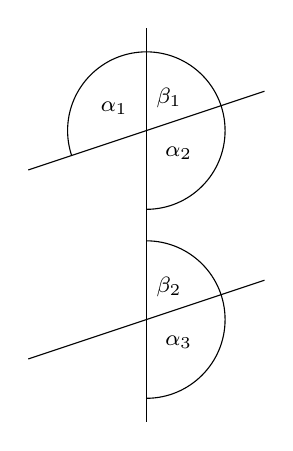
\begin{tikzpicture}
    \draw (1.5, 0.0) -- (1.5, 5.0);
    \draw (0.0, 3.2) -- (3.0, 4.2);
    \draw (0.0, 0.8) -- (3.0, 1.8);
    % Winkel oben
    \begin{scope}
      \clip (1.5, 3.7) --
            (0.0, 3.2) --
            (0.0, 5.0) --
            (3.0, 5.0) --
            (3.0, 1.8) --
            (1.5, 1.8) -- cycle;
      \draw (1.5, 3.7) circle (1cm);
      \node[shift=(145:5mm)] at (1.5, 3.7) {{\footnotesize$\alpha_{1}$}};
      \node[shift=(325:5mm)] at (1.5, 3.7) {{\footnotesize$\alpha_{2}$}};
      \node[shift=( 55:5mm)] at (1.5, 3.7) {{\footnotesize$\beta_{1}$}};
    \end{scope}
    % Winkel unten
    \begin{scope}
      \clip (1.5, 0.0) --
            (1.5, 2.5) --
            (3.0, 2.5) --
            (3.0, 0.0) -- cycle;
      \draw (1.5, 1.3) circle (1cm);
      \node[shift=(325:5mm)] at (1.5, 1.3) {{\footnotesize$\alpha_{3}$}};
      \node[shift=( 55:5mm)] at (1.5, 1.3) {{\footnotesize$\beta_{2}$}};
    \end{scope}
  \end{tikzpicture}
  \vspace*{\baselineskip}
\end{minipage}%
\hfill
\begin{minipage}[c]{0.54\linewidth}
  Nebenwinkel:
  \formrow{\alpha_{1}+\beta_{1}=180^{\circ}}

  Scheitelwinkel:
  \formrow{\alpha_{1}=\alpha_{2}}

  Stufenwinkel:
  \formrow{\beta_{1}=\beta_{2}}

  Wechselwinkel:
  \formrow{\alpha_{1}=\alpha_{3}}
\end{minipage}%


  % ------------------------
\mysec{Winkel im Bogenmaß}
% ------------------------
\begin{minipage}{0.44\linewidth}
  \centering
  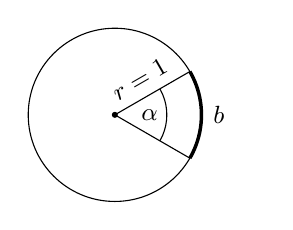
\begin{tikzpicture}[scale=1.1]
    \fill (0, 0) circle (1pt);
    \draw (0, 0) circle (1cm);
    \draw (30:1cm) -- (0, 0) -- (330:1cm);
    \begin{scope}
      \clip (30:2cm) -- (0, 0) -- (330:2cm);
      % Winkel
      \draw (0, 0) circle (6mm);
      % Bogenlaenge
      \draw[line width=1.25pt] (0, 0) circle (1cm);
    \end{scope}
    % Beschriftung
    \node at (0:4mm)  {{\small$\alpha$}};
    \node at (0:12mm) {{\small$b$}};
    \node[rotate=30] at (55:5mm) {{\small$r=1$}};
  \end{tikzpicture}
\end{minipage}%
\begin{minipage}{0.55\linewidth}
  \formrow{\frac{\alpha^{\circ}}{360^{\circ}}=\frac{b}{2\pi}}
  \formrow{\alpha^{\circ}=b\cdot\frac{180^{\circ}}{\pi}}
  \formrow{b=\alpha^{\circ}\cdot\frac{\pi}{180^{\circ}}}
\end{minipage}

\end{minipage}


\newpage
% ------------------------------------------------------------------------------
% Seite 4                                                                Seite 4
% ------------------------------------------------------------------------------
\begin{minipage}[t]{0.45\textwidth}
  % --------------------
\mysec{Kongruenzsätze}
% --------------------
\formnum \textbf{SSS:} Zwei Dreiecke, die in ihren drei Seitenlängen
übereinstimmen, sind kongruent.\medskip\par
\formnum \textbf{SWS:} Zwei Dreiecke, die in zwei Seitenlängen und in
dem eingeschlossenen Winkel übereinstimmen, sind kongruent.\medskip\par
\formnum \textbf{WSW:} Zwei Dreiecke, die in einer Seitenlänge und in
den dieser Seite anliegenden Winkeln übereinstimmen, sind kongruent.\medskip\par
\formnum \textbf{SsW:} Zwei Dreiecke, die in zwei Seitenlängen und in
jenem Winkel übereinstimmen, der der längeren Seite gegenüberliegt,
sind kongruent.\medskip\par
\begin{center}
  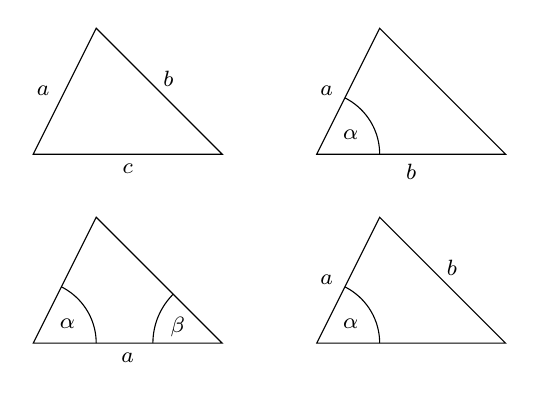
\begin{tikzpicture}[scale=0.8]
    \begin{scope}
      \draw (0, 0) -- (3, 0) -- (1, 2) -- cycle;
      \path (0, 0) -- node[below]{{\footnotesize$c$}}
            (3, 0) -- node[above right=-2pt]{{\footnotesize$b$}}
            (1, 2) -- node[left=2pt]{{\footnotesize$a$}}
            (0, 0);
    \end{scope}
    \begin{scope}[xshift=4.5cm]
      \draw (0, 0) -- (3, 0) -- (1, 2) -- cycle;
      \path (0, 0) -- node[below]{{\footnotesize$b$}}
            (3, 0) --
            (1, 2) -- node[left=2pt]{{\footnotesize$a$}}
            (0, 0);
      \begin{scope}
        \clip (0, 0) -- (3, 0) -- (1, 2) -- cycle;
        \draw (0, 0) circle (1cm);
        \node[shift=(30:5mm)] at (0, 0) {{\footnotesize$\alpha$}};
      \end{scope}
    \end{scope}
    \begin{scope}[yshift=-3cm]
      \draw (0, 0) -- node[below]{{\footnotesize$a$}}
            (3, 0) --
            (1, 2) -- cycle;
      \begin{scope}
        \clip (0, 0) -- (3, 0) -- (1, 2) -- cycle;
        \draw (0, 0) circle (1cm);
        \node[shift=(30:5mm)] at (0, 0) {{\footnotesize$\alpha$}};
      \end{scope}
      \begin{scope}
        \clip (0, 0) -- (3, 0) -- (1, 2) -- cycle;
        \draw (3, 0) circle (1.1cm);
        \node[shift=(160:6mm)] at (3, 0) {{\footnotesize$\beta$}};
      \end{scope}
    \end{scope}
    \begin{scope}[xshift=4.5cm, yshift=-3cm]
      \draw (0, 0) -- (3, 0) -- (1, 2) -- cycle;
      \path (0, 0) --
            (3, 0) -- node[above right=-2pt]{{\footnotesize$b$}}
            (1, 2) -- node[left=2pt]{{\footnotesize$a$}}
            (0, 0);
      \begin{scope}
        \clip (0, 0) -- (3, 0) -- (1, 2) -- cycle;
        \draw (0, 0) circle (1cm);
        \node[shift=(30:5mm)] at (0, 0) {{\footnotesize$\alpha$}};
      \end{scope}
    \end{scope}
  \end{tikzpicture}
\end{center}


  % -------------------------------
\mysec{Satzgruppe des Pythagoras}
% -------------------------------
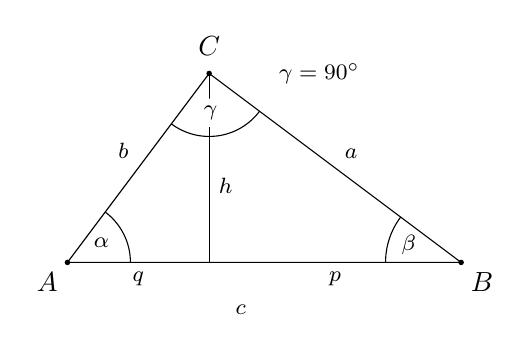
\begin{tikzpicture}[scale=0.2]
  % Linien
  \draw ( 0,  0) -- node[below]       {{\footnotesize$q$}}
        ( 9,  0) -- node[below]       {{\footnotesize$p$}}
        (25,  0) -- node[above right] {{\footnotesize$a$}}
        ( 9, 12) -- node[above left]  {{\footnotesize$b$}}
        ( 0,  0);
  \draw ( 9,  0) -- node[below right] {{\footnotesize$h$}}
        ( 9, 12);
  \node at (11, -3)                   {{\footnotesize$c$}};
  % Punkte
  \fill ( 0,  0) circle (5pt) node[below left]  {$A$};
  \fill (25,  0) circle (5pt) node[below right] {$B$};
  \fill ( 9, 12) circle (5pt) node[above=1mm]   {$C$};
  % alpha
  \begin{scope}
    \clip (0, 0) -- (25, 0) -- (9, 12) -- cycle;
    \draw (0, 0) circle (4);
    \node[shift=(30:5mm)] at (0, 0) {{\footnotesize$\alpha$}};
  \end{scope}
  % beta
  \begin{scope}
    \clip (0, 0) -- (25, 0) -- (9, 12) -- cycle;
    \draw (25, 0) circle (4.8);
    \node[shift=(162:7mm)] at (25, 0) {{\footnotesize$\beta$}};
  \end{scope}
  % gamma
  \begin{scope}
    \clip (0, 0) -- (25, 0) -- (9, 12) -- cycle;
    \draw (9, 12) circle (4);
    \fill[shift=(272:25mm), fill=white] (9, 12) circle (9mm);
    \node[shift=(272:5mm)] at (9, 12) {{\footnotesize$\gamma$}};
  \end{scope}
  \node at (16, 12) {{\footnotesize$\gamma=90^{\circ}$}};
\end{tikzpicture}\par\medskip
Satz des Pythagoras:\\[-0.75\baselineskip]
\formrow{c^{2}=a^{2}+b^{2}}

Höhensatz des Euklid:\\[-0.75\baselineskip]
\formrow{h^{2}=p\cdot q}

Kathetensatz des Euklid:\\[-0.75\baselineskip]
\formrow{a^{2}=p\cdot c}
\formrow{b^{2}=q\cdot c}


\end{minipage}%
\hfill
\begin{minipage}[t]{0.45\textwidth}
  % -------------------------
\mysec{Allgemeine Dreiecke}
% -------------------------
\begin{tikzpicture}
  \coordinate (A)  at (0, 0);
  \coordinate (B)  at (6, 0);
  \coordinate (Ca) at (60:6cm);
  \coordinate (Cb) at ([xshift=6cm]140:6cm);
  \coordinate (C)  at (intersection of A--Ca and B--Cb);
  \coordinate (Fa) at ([shift={(270:6cm)}]C);
  \coordinate (F)  at (intersection of A--B and C--Fa);
  % Dreiecksseiten
  \draw (A) -- node[shift={(270:3mm)}] {{\footnotesize$c$}} (B);
  \draw (B) -- node[shift={(50:3mm)}]  {{\footnotesize$a$}} (C);
  \draw (C) -- node[shift={(150:3mm)}] {{\footnotesize$b$}} (A);
  % Hoehe
  \draw (C) -- node[shift={(0:3mm)}] {{\footnotesize$h_{c}$}} (F);
  % rechter Winkel
  \begin{scope}
    \clip (F) -- (B) -- (C) -- cycle;
    \draw (F) circle (5mm);
    \fill ([shift={(45:2.75mm)}]F) circle (1.1pt);
  \end{scope}
  % Eckpunkte
  \fill (A) circle (1pt);
  \fill (B) circle (1pt);
  \fill (C) circle (1pt);
  % Beschriftung der Eckpunkte
  \node[shift={(220:3mm)}] at (A) {{\footnotesize$A$}};
  \node[shift={(320:3mm)}] at (B) {{\footnotesize$B$}};
  \node[shift={(90:3mm)}]  at (C) {{\footnotesize$C$}};
  % Winkel
  \begin{scope}
    \clip (A) -- (B) -- (C) -- cycle;
    \draw (A) circle (8mm);
    \draw (B) circle (9mm);
    \draw (C) circle (8mm);
    \node[shift={(30:5mm)}]              at (A) {{\footnotesize$\alpha$}};
    \node[shift={(160:6mm)}]             at (B) {{\footnotesize$\beta$}};
    \node[shift={(280:5mm)}, fill=white] at (C) {{\footnotesize$\gamma$}};
  \end{scope}
\end{tikzpicture}

Fläche:\medskip
\formrow{A=\frac{c\cdot h_{c}}{2}=\frac{a\cdot h_{a}}{2}=\frac{b\cdot h_{b}}{2}}

Innenwinkelsumme:\medskip
\formrow{\alpha+\beta+\gamma=180^{\circ}}

Sinussatz:\medskip\par
\formrow{\frac{a}{\sin\alpha}=\frac{b}{\sin\beta}=\frac{c}{\sin\gamma}=2r_{u}}

Kosinussatz:\medskip\par
\formrow{c^{2}=a^{2}+b^{2}-2ab\cdot\cos\gamma}

Schnittpunkte:\medskip\par
\begingroup\small
\begin{tabular}{ll}
Höhen              &                               \\
Seitenhalbierenden & \itshape (Schwerpunkt)        \\
Winkelhalbierenden & \itshape (Inkreismittelpunkt) \\
Mittelsenkrechten  & \itshape (Umkreismittelpunkt)
\end{tabular}
\endgroup


  % ------------------
\mysec{Strahlensatz}
% ------------------
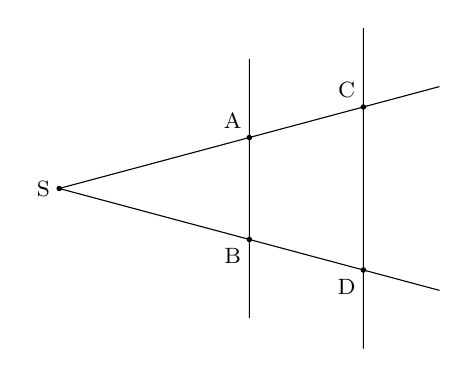
\begin{tikzpicture}[rotate=-15]
  \draw (0.0, 0) -- (5.0000, 0.0000); % unterer Strahl
  \draw (0.0, 0) -- (4.3301, 2.5000); % oberer Strahl
  \draw (1.90620,  2.21590) -- (2.75882, -0.96593); % erste Parallele
  \draw (3.20530,  2.96590) -- (4.25882, -0.96593); % zweite Parallele
  \fill (0.000, 0.000) circle (1pt); % S
  \fill (2.500, 0.000) circle (1pt); % B
  \fill (4.000, 0.000) circle (1pt); % D
  \fill (3.464, 2.000) circle (1pt); % C
  \fill (2.165, 1.250) circle (1pt); % A
  \node[shift=(180:2mm)] at (0.000, 0.000) {{\footnotesize S}};
  \node[shift=(135:3mm)] at (2.165, 1.250) {{\footnotesize A}};
  \node[shift=(225:3mm)] at (2.500, 0.000) {{\footnotesize B}};
  \node[shift=(135:3mm)] at (3.464, 2.000) {{\footnotesize C}};
  \node[shift=(225:3mm)] at (4.000, 0.000) {{\footnotesize D}};
\end{tikzpicture}\bigskip
\formrow{\frac{\;\overline{SA}\;}{\overline{SC}}=\frac{\;\overline{SB}\;}{\overline{SD}}=\frac{\;\overline{AB}\;}{\overline{CD}}}
\formrow{\frac{\;\overline{AC}\;}{\overline{SC}}=\frac{\;\overline{BD}\;}{\overline{SD}}}
\formrow{\frac{\;\overline{SA}\;}{\overline{AC}}=\frac{\;\overline{SB}\;}{\overline{BD}}}


\end{minipage}


\newpage
% ------------------------------------------------------------------------------
% Seite 5                                                                Seite 5
% ------------------------------------------------------------------------------
% --------------
\mysec{Vierecke}
% --------------
\begin{minipage}[t]{0.25\textwidth}
Quadrat:\medskip\par
\begin{tikzpicture}
  % Hintergrund
  \begin{scope}[xshift=-0.5cm, yshift=-0.5cm]
    \fill[fill=white] (0.0, 0.0) rectangle (2.5, 2.5);
  \end{scope}
  \coordinate (A) at (0.0, 0.0);
  \coordinate (B) at (1.5, 0.0);
  \coordinate (C) at (1.5, 1.5);
  \coordinate (D) at (0.0, 1.5);
  \draw (A) -- node[below] {{\footnotesize$a$}}
        (B) -- node[right] {{\footnotesize$a$}}
        (C) -- (D) -- cycle;
\end{tikzpicture}
\formrow{U=4a}
\formrow{A=a^{2}}
\end{minipage}%
\hfill
\begin{minipage}[t]{0.30\textwidth}
Rechteck:\medskip\par
\begin{tikzpicture}
  % Hintergrund
  \begin{scope}[xshift=-0.5cm, yshift=-0.5cm]
    \fill[fill=white] (0.0, 0.0) rectangle (4.0, 2.5);
  \end{scope}
  \coordinate (A) at (0.0, 0.0);
  \coordinate (B) at (3.0, 0.0);
  \coordinate (C) at (3.0, 1.5);
  \coordinate (D) at (0.0, 1.5);
  \draw (A) -- node[below] {{\footnotesize$a$}}
        (B) -- node[right] {{\footnotesize$b$}}
        (C) -- (D) -- cycle;
\end{tikzpicture}
\formrow{U=2(a+b)}
\formrow{A=a\cdot b}
\end{minipage}%
\hfill
\begin{minipage}[t]{0.30\textwidth}
Trapez:\medskip\par
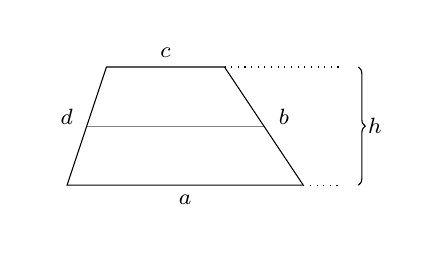
\begin{tikzpicture}
  % Hintergrund
  \begin{scope}[xshift=-0.5cm, yshift=-0.5cm]
    \fill[fill=white] (0.0, 0.0) rectangle (4.75, 2.5);
  \end{scope}
  \coordinate (A) at (0.00,  0.00);
  \coordinate (B) at (3.00,  0.00);
  \coordinate (C) at (2.00,  1.50);
  \coordinate (D) at (0.50,  1.50);
  \coordinate (E) at ($(A)!0.5!(D)$);
  \coordinate (F) at ($(B)!0.5!(C)$);
  \coordinate (H) at (3.50,  0.00);
  \coordinate (I) at (3.50,  1.50);
  % Mittellinie
  \draw[draw=black!50!white] (E) -- (F);
  % das Trapez
  \draw (A) -- (B) -- (C) -- (D) -- cycle;
  % Hilfslinien
  \draw[dotted] (B) -- (H);
  \draw[dotted] (C) -- (I);
  % Bezeichnungen
  \path (A) -- node[below]            {{\footnotesize$a$}} (B);
  \path (B) -- node[shift=(25:8pt)]   {{\footnotesize$b$}} (C);
  \path (C) -- node[above]            {{\footnotesize$c$}} (D);
  \path (D) -- node[shift=(155:8pt)]  {{\footnotesize$d$}} (A);
  % Hoehe
  \draw[decorate, decoration=brace] ([xshift=2mm]I) -- node[right]{{\footnotesize$h$}} ([xshift=2mm]H);
\end{tikzpicture}
\formrow{U=a+b+c+d}
\formrow{A=\frac{a+c}{2}\cdot h}
\end{minipage}%

\begin{minipage}[t]{0.25\textwidth}
Raute:\medskip\par
\begin{tikzpicture}
  % Hintergrund
  \begin{scope}[xshift=-0.5cm, yshift=-0.5cm]
    \fill[fill=white] (0.0, 0.0) rectangle (3.5, 2.5);
  \end{scope}
  \coordinate                            (A) at (0.0, 0.0);
  \coordinate                            (B) at (1.5, 0.0);
  \coordinate[xshift=1.5cm]              (C) at (55:1.5cm);
  \coordinate                            (D) at (55:1.5cm);
  \coordinate                            (E) at (9.0, 0.0);
  \coordinate[xshift=1.5cm, yshift=-9cm] (F) at (55:1.5cm);
  \coordinate                            (H) at (intersection of A--E and C--F);
  \draw[dotted] (B) -- (H);
  \draw[decorate, decoration=brace] ([xshift=2mm]C) -- node[right]{{\footnotesize$h$}} ([xshift=2mm]H);
  \draw (A) -- node[below] {{\footnotesize$a$}}
        (B) -- (C) -- (D) -- cycle;
  \path (A) -- node[above left] {{\footnotesize$a$}} (D);
\end{tikzpicture}
\formrow{U=4a}
\formrow{A=a\cdot h}
\end{minipage}%
\hfill
\begin{minipage}[t]{0.30\textwidth}
Parallelogramm:\medskip\par
\begin{tikzpicture}
  % Hintergrund
  \begin{scope}[xshift=-0.5cm, yshift=-0.5cm]
    \fill[fill=white] (0.0, 0.0) rectangle (4.5, 2.5);
  \end{scope}
  \coordinate                            (A) at (0.0, 0.0);
  \coordinate                            (B) at (2.5, 0.0);
  \coordinate[xshift=2.5cm]              (C) at (55:1.5cm);
  \coordinate                            (D) at (55:1.5cm);
  \coordinate                            (E) at (9.0, 0.0);
  \coordinate[xshift=2.5cm, yshift=-9cm] (F) at (55:1.5cm);
  \coordinate                            (H) at (intersection of A--E and C--F);
  \draw[dotted] (B) -- (H);
  \draw[decorate, decoration=brace] ([xshift=2mm]C) -- node[right]{{\footnotesize$h$}} ([xshift=2mm]H);
  \draw (A) -- node[below] {{\footnotesize$a$}}
        (B) -- (C) -- (D) -- cycle;
  \path (A) -- node[above left] {{\footnotesize$b$}} (D);
\end{tikzpicture}
\formrow{U=2(a+b)}
\formrow{A=a\cdot h}
\end{minipage}%
\hfill
\begin{minipage}[t]{0.30\textwidth}
Drachen:\medskip\par
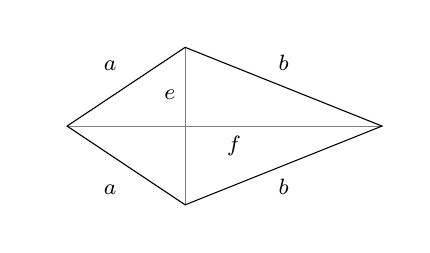
\begin{tikzpicture}
  % Hintergrund
  \begin{scope}[xshift=-0.5cm, yshift=-1.25cm]
    \fill[fill=white] (0.0, 0.0) rectangle (4.75, 2.5);
  \end{scope}
  \newcommand{\vstrut}{\rule[-0.7ex]{0pt}{2.7ex}}
  \coordinate (A) at (0.00,  0.00);
  \coordinate (B) at (1.50, -1.00);
  \coordinate (C) at (4.00,  0.00);
  \coordinate (D) at (1.50,  1.00);
  \coordinate (E) at ($(B)!0.70!(D)$);
  \coordinate (F) at ($(A)!0.53!(C)$);
  \draw[draw=black!50!white] (A) -- (C);
  \draw[draw=black!50!white] (B) -- (D);
  \draw (A) -- (B) -- (C) -- (D) -- cycle;
  \path (A) -- node[below left] {{\footnotesize\vstrut$a$}} (B);
  \path (B) -- node[below]      {{\footnotesize\vstrut$b$}} (C);
  \path (C) -- node[above]      {{\footnotesize\vstrut$b$}} (D);
  \path (D) -- node[above left] {{\footnotesize\vstrut$a$}} (A);
  \node[left] at (E) {{\footnotesize$e$}};
  \node[below] at (F) {{\footnotesize$f$}};
\end{tikzpicture}
\formrow{U=2(a+b)}
\formrow{A=\frac{e\cdot f}{2}}
\end{minipage}


\begin{minipage}[t]{0.47\textwidth}
  % --------------------
\mysec{Kreise}\bigskip
% --------------------
\begin{minipage}[c]{0.30\textwidth}
  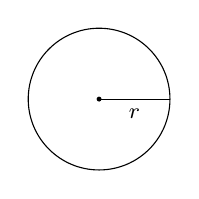
\begin{tikzpicture}[scale=0.9]
    \draw (0, 0) circle (1cm);
    \draw (0, 0) -- node[below]{{\footnotesize$r$}} (1, 0);
    \fill (0, 0) circle (1pt);
  \end{tikzpicture}
\end{minipage}%
\begin{minipage}[c]{0.70\textwidth}
  \formrow{U=2\pi r}
  \formrow{A=\pi r^{2}}\vspace*{-\bigskipamount}
\end{minipage}\bigskip

Kreisbogen:\medskip\par
\begin{minipage}[c]{0.30\textwidth}
  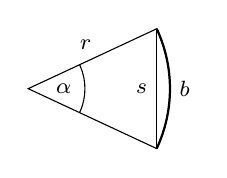
\begin{tikzpicture}[scale=0.9]
    \node[shift=(115:2mm)] at (25:1cm) {{\footnotesize$r$}};
    \node[right] at (2, 0) {{\footnotesize$b$}};
    % Winkel
    \begin{scope}
      \clip (0, 0) -- (-25:2cm) arc (-25:25:2cm) -- cycle;
      \draw (0, 0) circle (8mm);
      \node at (0:5mm) {{\footnotesize$\alpha$}};
    \end{scope}
    % Sehne
    \draw (-25:2cm) -- node[left]{{\footnotesize$s$}}(25:2cm);
    \draw (0, 0) -- (-25:2cm) arc (-25:25:2cm) -- cycle;
    \draw[line width=0.8pt] (-25:2cm) arc (-25:25:2cm);
  \end{tikzpicture}
\end{minipage}%
\begin{minipage}[c]{0.70\textwidth}
  \formrow{b=\frac{\pi\alpha}{180}\cdot r}
  \formrow{s=2r\cdot\sin\frac{\alpha}{2}}\vspace*{-\bigskipamount}
\end{minipage}\bigskip

Kreisausschnitt:\medskip\par
\begin{minipage}[c]{0.30\textwidth}
  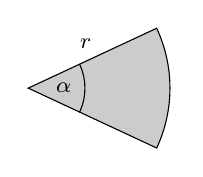
\begin{tikzpicture}[scale=0.9]
    \node[shift=(115:2mm)] at (25:1cm) {{\footnotesize$r$}};
    % Flaeche
    \fill[fill=white!80!black] (0, 0) -- (-25:2cm) arc (-25:25:2cm) -- cycle;
    % Winkel
    \begin{scope}
      \clip (0, 0) -- (-25:2cm) arc (-25:25:2cm) -- cycle;
      \draw (0, 0) circle (8mm);
      \node at (0:5mm) {{\footnotesize$\alpha$}};
    \end{scope}
    \draw (0, 0) -- (-25:2cm) arc (-25:25:2cm) -- cycle;
  \end{tikzpicture}
\end{minipage}%
\begin{minipage}[c]{0.70\textwidth}
  \formrow{A=\frac{\pi\alpha}{360}\cdot r^{2}}\vspace*{-\bigskipamount}
\end{minipage}\bigskip

Kreisabschnitt:\medskip\par
\begin{minipage}[c]{0.30\textwidth}
  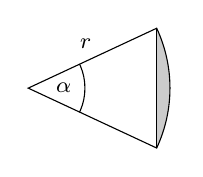
\begin{tikzpicture}[scale=0.9]
    \node[shift=(115:2mm)] at (25:1cm) {{\footnotesize$r$}};
    % Flaeche
    \fill[fill=white!80!black] (-25:2cm) arc (-25:25:2cm) -- cycle;
    % Winkel
    \begin{scope}
      \clip (0, 0) -- (-25:2cm) arc (-25:25:2cm) -- cycle;
      \draw (0, 0) circle (8mm);
      \node at (0:5mm) {{\footnotesize$\alpha$}};
    \end{scope}
    \draw (0, 0) -- (-25:2cm) arc (-25:25:2cm) -- cycle;
    % Sehne
    \draw (-25:2cm) -- (25:2cm);
  \end{tikzpicture}
\end{minipage}%
\begin{minipage}[c]{0.70\textwidth}
  \formrow{A=\frac{r^{2}}{2}\cdot\left(\frac{\pi\alpha}{180}-\sin\alpha\right)}\vspace*{-\bigskipamount}
\end{minipage}


\end{minipage}%
\hfill
\begin{minipage}[t]{0.45\textwidth}
  % -------------------------------------------
\mysec{Körper mit gekrümmten Flächen}\bigskip
% -------------------------------------------
Kugel:\medskip\par
\begin{minipage}{0.35\linewidth}
  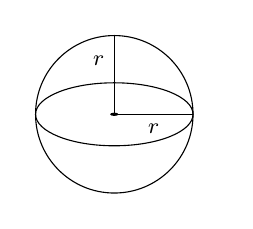
\begin{tikzpicture}
    \clip (-1.1, -1.1) rectangle (1.4, 1.1);
    \draw (0, 0) circle (1);
    \draw (0, 0) -- node[below]{{\footnotesize$r$}} (1, 0);
    \draw (0, 0) -- node[above left]{{\footnotesize$r$}} (0, 1);
    \fill (0, 0) ellipse (1.5pt and 0.6pt);
    \draw (0, 0) ellipse (1 and 0.4);
  \end{tikzpicture}%
\end{minipage}%
\begin{minipage}{0.65\linewidth}
  \formrow{O=4\pi r^{2}}
  \formrow{V=\frac{4}{3}\pi r^{3}}\vspace*{-\bigskipamount}
\end{minipage}\bigskip

Zylinder:\medskip\par
\begin{minipage}{0.35\linewidth}
  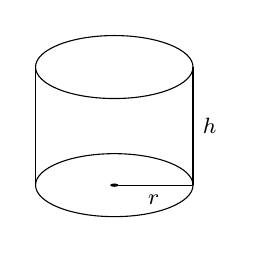
\begin{tikzpicture}
    \clip (-1.1, -0.5) rectangle (1.4, 2.0);
    \draw (-1, 0) -- (-1, 1.5);
    \draw (1, 0) -- node[right]{{\footnotesize$h$}} (1, 1.5);
    \draw (0, 1.5) ellipse (1 and 0.4);
    \draw (0, 0) ellipse (1 and 0.4);
    \draw (0, 0) -- node[below]{{\footnotesize$r$}} (1, 0);
    \fill (0, 0) ellipse (1.5pt and 0.6pt);
  \end{tikzpicture}%
\end{minipage}%
\begin{minipage}{0.65\linewidth}
  \formrow{O=2\pi r^{2}+2\pi rh}
  \formrow{V=\pi r^{2}h}\vspace*{-\bigskipamount}
\end{minipage}\bigskip

Kegel:\medskip\par
\begin{minipage}{0.35\linewidth}
  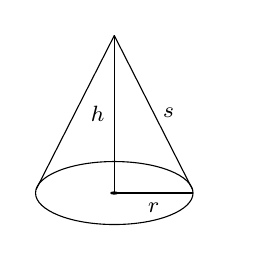
\begin{tikzpicture}
    \clip (-1.1, -0.5) rectangle (1.4, 2.1);
    \draw (0, 0) ellipse (1 and 0.4);
    \draw[cap=round] ([shift=(80:0.5mm)]-1, 0) -- (0, 2);
    \draw[cap=round] ([shift=(100:0.5mm)]1, 0) -- node[right]{{\footnotesize$s$}} (0, 2);
    \draw (0, 0) -- node[below]{{\footnotesize$r$}} (1, 0);
    \draw (0, 0) -- node[left]{{\footnotesize$h$}} (0, 2);
    \fill (0, 0) ellipse (1.5pt and 0.6pt);
  \end{tikzpicture}%
\end{minipage}%
\begin{minipage}{0.65\linewidth}
  \formrow{O=\pi r^{2}+\pi rs}
  \formrow{V=\frac{1}{3}\pi r^{2}h}\vspace*{-\bigskipamount}
\end{minipage}


\end{minipage}

\newpage
% -----------------
\mysec{Mittelwerte}
% -----------------
\begin{minipage}[t]{0.48\textwidth}
  Arithmetisches Mittel:\medskip
  \formrow{\bar{x}=\frac{1}{n}\left(x_{1}+x_{2}+\dotsb+x_{n}\right)}

  Geometisches Mittel:\medskip
  \formrow{\bar{x}=\sqrt[n]{x_{1}\cdot x_{2}\cdot\dotsb\cdot x_{n}}}
\end{minipage}\hfill
\begin{minipage}[t]{0.48\textwidth}
  Median:\medskip
  \formrow
  {
    \bar{x}=\left\{
            \begin{array}{ll}
              x_{\frac{n+1}{2}}                                         & \text{$n$ ungerade} \\[2ex]
              \frac{1}{2}\left(x_{\frac{n}{2}}+x_{\frac{n}{2}+1}\right) & \text{$n$ gerade}
            \end{array}
            \right.
  }
\end{minipage}

% -------------------
\mysec{Skalenniveaus}
% -------------------
\begin{center}
  \renewcommand{\arraystretch}{1.5}
  \begin{tabular}{|ll|l|l|}
    \hline
    \multicolumn{2}{|l|}{\textbf{Skalenniveau}} & \textbf{Operationen}            & \textbf{Mittelwerte}  \\
    \hline
    \multicolumn{2}{|l|}{Nominalskala}          & $=\;\neq$                       & Modus                 \\
    \hline
    \multicolumn{2}{|l|}{Ordinalskala}          & $=\;\neq\;<\;>$                 & Median                \\
    \hline
    \multirow{2}{*}{Kardinalskala}
      & \multicolumn{1}{|l|}{Intervallskala}    & $=\;\neq\;<\;>\;+\;-$           & arithmetisches Mittel \\
      \cline{2-4}
      & \multicolumn{1}{|l|}{Rationalskala}     & $=\;\neq\;<\;>\;+\;-\;\cdot\;:$ & geometrisches Mittel  \\
    \hline
  \end{tabular}
\end{center}

\formnum \textbf{Nominalskalierte Merkmale:} Deren mögliche Ausprägungen
können zwar unterschieden werden, weisen aber keine natürliche Rangfolge auf.
\begin{itemize}
  \setlength{\itemsep}{-0.5\baselineskip}
  \item Geschlecht: männlich, weiblich
  \item Geburtsort: Hamburg, Berlin, München
  \item Familienstand: ledig, verlobt, verheiratet, geschieden, verwitwet
  \item Religionszugehörigkeit: evangelisch, katholisch, muslimisch
\end{itemize}
\medskip\par

\formnum \textbf{Ordinalskalierte Merkmale:} Deren mögliche Ausprägungen können
unterschieden werden und weisen darüber hinaus eine natürliche Rangfolge auf.
\begin{itemize}
  \setlength{\itemsep}{-0.5\baselineskip}
  \item Schulnoten: sehr gut, gut, befriedigend, ausreichend, mangelhaft, ungenügend
  \item Musik-Charts: Platz 1, Platz 2, \ldots
  \item Schadstoffgruppen für Kraftfahrzeuge: 1, 2, 3, 4
  \item Dienstgrade beim Militär: Admiral, \ldots, Matrose
\end{itemize}
\medskip\par

\formnum \textbf{Intervallskalierte Merkmale:} Deren mögliche Ausprägungen
können so quantifiziert werden, dass gleichen Differenzen der Messwerte immer
gleichgroße Merkmalsunterschiede von je zwei Objekten entsprechen.
\begin{itemize}
  \setlength{\itemsep}{-0.5\baselineskip}
  \item Temperatur in ${}^{\circ}C$ oder ${}^{\circ}\!F$
  \item Kalenderzeit
  \item IQ-Skala
\end{itemize}
\medskip\par

\formnum \textbf{Rationalskalierte Merkmale:} Deren mögliche Ausprägungen
können so quantifiziert werden, dass der Markmalswert exakt dem Abstand zu
einem absoluten Nullpunkt entspricht.
\begin{itemize}
  \setlength{\itemsep}{-0.5\baselineskip}
  \item Temperatur in ${}^{\circ}\!K$
  \item Anzahl, Größe, Gewicht
  \item Preise
\end{itemize}


\newpage
\begin{minipage}[t]{0.45\textwidth}
  % ------------------
  \mysec{Kombinatorik}
  % ------------------
  \paragraph{Permutation:} Gesucht wird die Anzahl der unterschiedlichen Reihenfolgen,
  in denen man die Elemente einer $n$-elementigen Menge $\Omega$ anordnen kann.
  \begin{itemize}
    \item Sind alle $n$ Objekte in $\Omega$ unterscheidbar, beträgt die
          Anzahl $a$ der Permutationen
          \formrow{a=n!}\newline
          \textit{10 verschiedene Bücher lassen sich auf $10!=3\,628\,800$
          unterschiedliche Arten in ein Bücherregal stellen.}
    \item Gibt es $g$ Gruppen in $\Omega$ mit jeweils $m_{1},\ldots,m_{g}$
          identischen Objekten, reduziert sich die Anzahl $a$ der Permutation auf
          \formrow{a=\frac{n!}{m_{1}!\cdot m_{2}!\dotsb m_{g}!}}\newline
          \textit{Aus 3 roten, 4 blauen und 5 gelben Legosteinen lassen sich}
          \begin{equation*}
            \frac{(3+4+5)!}{3!\cdot4!\cdot5!}=27\,720
          \end{equation*}
          \textit{Türme mit unterschiedlichem Farbmuster bauen.}
  \end{itemize}
  \paragraph{Variation:} Gesucht wird die Anzahl der voneinander verschiedenen
  Tupel, die man aus $k$ Elementen einer $n$-elementigen Menge $\Omega$
  bilden kann.
  \begin{itemize}
    \item Darf jedes Element aus $\Omega$ höchstens einmal ausgewählt
          werden, beträgt die Anzahl $a$ der Variationen
          \formrow{a=\frac{n!}{(n-k)!}}\newline
          \textit{Wenn für 10 verschiedene Autos 5 freie Parkplätze zur Verfügung stehen, gibt es}
          \begin{equation*}
            \frac{10!}{(10-5)!}=30\,240
          \end{equation*}
          \textit{verschiedene Möglichkeiten die Parkplätze zu belegen.}
  \end{itemize}
\end{minipage}%
\hfill
\begin{minipage}[t]{0.45\textwidth}
  \begin{itemize}
    \item Wird jedes Element nach der Ziehung wieder zurück in die Menge $\Omega$
          gelegt, beträgt die Anzahl $a$ der Variationen
          \formrow{a=n^{k}}\newline
          \textit{Auf einem fünfstelligen Zahlenschloss mit den Ziffern 0 bis 9
          auf jedem Ring lassen sich $10^{5}=100\,000$ verschiedene Zahlencodes
          einstellen.}
  \end{itemize}
  \paragraph{Kombination:} Gesucht wird die Anzahl der voneinander
  verschiedenen Mengen, die man aus $k$ Elementen einer $n$-elementigen
  Menge $\Omega$ bilden kann.
  \begin{itemize}
    \item Darf jedes Element aus $\Omega$ höchstens einmal ausgewählt
          werden, beträgt die Anzahl $a$ der Kombinationen\medskip
          \formrow{a=\binom{n}{k}=\frac{n!}{(n-k)!\cdot k!}}\newline
          \textit{Beim Lottospiel \glqq 6 aus 49\grqq{} gibt es}
          \begin{equation*}
            \binom{49}{6}=\frac{49!}{(49-6)!\cdot 6!}=13\,983\,816
          \end{equation*}
          \textit{verschiedene Möglichkeiten 6 aus 49 Zahlen auszuwählen.}
    \item Wird jedes Element nach der Ziehung wieder zurück in die Menge $\Omega$
          gelegt, beträgt die Anzahl $a$ der Kombinationen\medskip
          \formrow{a=\binom{n+k-1}{k}}\newline
          \textit{Wenn 10 nicht voneinander unterscheidbare Raben die Möglichkeit
          haben sich auf 5 verschiedene Bäume zu setzen, dann lassen sich}
          \begin{equation*}
            \binom{5+10-1}{10}=\binom{14}{10}=1001
          \end{equation*}
          \textit{unterschiedliche Verteilungen beobachten.}
  \end{itemize}
\end{minipage}


\newpage
% ---------------------------------
\mysec{Trigonometrische Funktionen}
% ---------------------------------
\begin{center}
\begin{tikzpicture}
  \clip (-7.5, -3.3) rectangle (7.5, 3.7);
  \newcommand{\xmark}[1]{\draw (#1, 1mm) -- (#1, -1mm);}
  \begin{scope}
    \draw[style=dotted] (-6.2832, 2.95) node[above]{{\footnotesize$-2\pi\phantom{-}$}}           -- (-6.2832, -2.75) node[below]{{\footnotesize$-360^{\circ}$}};
    \draw[style=dotted] (-4.7124, 2.95) node[above]{{\footnotesize$-\frac{3\pi}{2}\phantom{-}$}} -- (-4.7124, -2.75) node[below]{{\footnotesize$-270^{\circ}$}};
    \draw[style=dotted] (-3.1416, 2.95) node[above]{{\footnotesize$-\pi\phantom{-}$}}            -- (-3.1416, -2.75) node[below]{{\footnotesize$-180^{\circ}$}};
    \draw[style=dotted] (-1.5708, 2.95) node[above]{{\footnotesize$-\frac{\pi}{2}\phantom{-}$}}  -- (-1.5708, -2.75) node[below]{{\footnotesize$-90^{\circ}$}};
    \draw[style=dotted] ( 1.5708, 2.95) node[above]{{\footnotesize$\frac{\pi}{2}$}}              -- ( 1.5708, -2.75) node[below]{{\footnotesize$90^{\circ}$}};
    \draw[style=dotted] ( 3.1416, 2.95) node[above]{{\footnotesize$\pi$}}                        -- ( 3.1416, -2.75) node[below]{{\footnotesize$180^{\circ}$}};
    \draw[style=dotted] ( 4.7124, 2.95) node[above]{{\footnotesize$\frac{3\pi}{2}$}}             -- ( 4.7124, -2.75) node[below]{{\footnotesize$270^{\circ}$}};
    \draw[style=dotted] ( 6.2832, 2.95) node[above]{{\footnotesize$2\pi$}}                       -- ( 6.2832, -2.75) node[below]{{\footnotesize$360^{\circ}$}};
  \end{scope}
  \begin{scope}[yshift=1.5cm]
    \draw[style=dotted] (-6.75,  1) node[left]{{\footnotesize$1$}}  -- (6.75,  1);
    \draw[style=dotted] (-6.75, -1) node[left]{{\footnotesize$-1$}} -- (6.75, -1);
    \draw[->, >=latex] (-6.75, 0) -- (6.75, 0) node[below]{{\footnotesize$\alpha$}};
    \draw[->, >=latex] (0, -1.25) -- (0, 1.45) node[below left]{{\footnotesize$\sin\alpha$}};
    \draw plot[smooth] file{sin.x};
    \xmark{-6.2832}; % -360
    \xmark{-4.7124}; % -270
    \xmark{-3.1416}; % -180
    \xmark{-1.5708}; %  -90
    \xmark{ 1.5708}; %   90
    \xmark{ 3.1416}; %  180
    \xmark{ 4.7124}; %  270
    \xmark{ 6.2832}; %  360
  \end{scope}
  \begin{scope}[yshift=-1.5cm]
    \draw[style=dotted] (-6.75,  1) node[left]{{\footnotesize$1$}}  -- (6.75,  1);
    \draw[style=dotted] (-6.75, -1) node[left]{{\footnotesize$-1$}} -- (6.75, -1);
    \draw[->, >=latex] (-6.75, 0) -- (6.75, 0) node[below]{{\footnotesize$\alpha$}};
    \draw[->, >=latex] (0, -1.25) -- (0, 1.45) node[below left]{{\footnotesize$\cos\alpha$}};
    \draw plot[smooth] file{cos.x};
    \xmark{-6.2832}; % -360
    \xmark{-4.7124}; % -270
    \xmark{-3.1416}; % -180
    \xmark{-1.5708}; %  -90
    \xmark{ 1.5708}; %   90
    \xmark{ 3.1416}; %  180
    \xmark{ 4.7124}; %  270
    \xmark{ 6.2832}; %  360
  \end{scope}
\end{tikzpicture}
\end{center}
\begin{minipage}[t]{0.45\textwidth}
Definitionen:\medskip
\formrow{\sin\alpha=\frac{\text{Gegenkathete}}{\text{Hypotenuse}}}
\formrow{\cos\alpha=\frac{\text{Ankathete}}{\text{Hypotenuse}}}
\formrow{\tan\alpha=\frac{\text{Gegenkathete}}{\text{Ankathete}}=\frac{\sin\alpha}{\cos\alpha}}
\formrow{\cot\alpha=\frac{\text{Ankathete}}{\text{Gegenkathete}}=\frac{\cos\alpha}{\sin\alpha}}

Periodizität ($k\in\mathbb{Z})$:\medskip
\formrow{\sin x=\sin(x+k\cdot2\pi)}
\formrow{\cos x=\cos(x+k\cdot2\pi)}
\formrow{\tan x=\tan(x+k\cdot\pi)}
\formrow{\cot x=\cot(x+k\cdot\pi)}

Symmetrie:\medskip
\formrow{\sin(-x)=-\sin x}\hfill(ungerade)
\formrow{\cos(-x)= \cos x}\hfill(gerade)
\formrow{\tan(-x)=-\tan x}\hfill(ungerade)
\formrow{\cot(-x)=-\cot x}\hfill(ungerade)
\end{minipage}%
\hfill
\begin{minipage}[t]{0.45\textwidth}
Grundformeln:\medskip
\formrow{\sin x=\cos(x-90^{\circ})}
\formrow{\cos x=\sin(x+90^{\circ})}
\formrow{\sin^{2}x+\cos^{2}x=1}

Additionstheoreme:\medskip
\formrow{\sin(x\pm y)=\sin x\cos y\pm\cos x\sin y}
\formrow{\cos(x\pm y)=\cos x\cos y\mp\sin x\sin y}

%Doppelter Winkel:\medskip
%\formrow{\sin 2x=2\sin x\cos x}
%\formrow{\cos 2x=\cos^{2}x-\sin^{2}x}

Spezielle Werte:\medskip\par
\begingroup
\renewcommand{\arraystretch}{1.4}
\setlength{\tabcolsep}{0.8em}
\begin{tabular}{rcccc}
                & $\sin$                & $\cos$                & $\tan$               & $\cot$                \\
    $0^{\circ}$ & $0$                   & $1$                   & $0$                  & $\pm\infty$           \\
   $30^{\circ}$ & $\frac{1}{2}$         & $\frac{\sqrt{3}}{2}$  & $\frac{\sqrt{3}}{3}$ & $\sqrt{3}$            \\
   $45^{\circ}$ & $\frac{\sqrt{2}}{2}$  & $\frac{\sqrt{2}}{2}$  & $1$                  & $1$                   \\
   $60^{\circ}$ & $\frac{\sqrt{3}}{2}$  & $\frac{1}{2}$         & $\sqrt{3}$           & $\frac{\sqrt{3}}{3}$  \\
   $90^{\circ}$ & $1$                   & $0$                   & $\pm\infty$          & $0$                   \\
  $120^{\circ}$ & $\frac{\sqrt{3}}{2}$  & $-\frac{1}{2}$        & $-\sqrt{3}$          & $-\frac{\sqrt{3}}{3}$ \\
  $135^{\circ}$ & $\frac{\sqrt{2}}{2}$  & $-\frac{\sqrt{2}}{2}$ & $-1$                 & $-1$                  \\
  $180^{\circ}$ & $0$                   & $-1$                  & $0$                  & $\pm\infty$           \\
  $225^{\circ}$ & $-\frac{\sqrt{2}}{2}$ & $-\frac{\sqrt{2}}{2}$ & $1$                  & $1$                   \\
  $270^{\circ}$ & $-1$                  & $0$                   & $\pm\infty$          & $0$                   \\
  $315^{\circ}$ & $-\frac{\sqrt{2}}{2}$ & $\frac{\sqrt{2}}{2}$  & $-1$                 & $-1$                  \\
\end{tabular}
\endgroup
\end{minipage}


\newpage
% ------------------------------------------------
\mysec{Seiten und Winkel in allgemeinen Dreiecken}
% ------------------------------------------------

\begin{minipage}[t]{4cm}
  \centering
  \begingroup
    \usekomafont{sectioning}%
    \usekomafont{paragraph}%
    SWS\bigskip\par
  \endgroup
  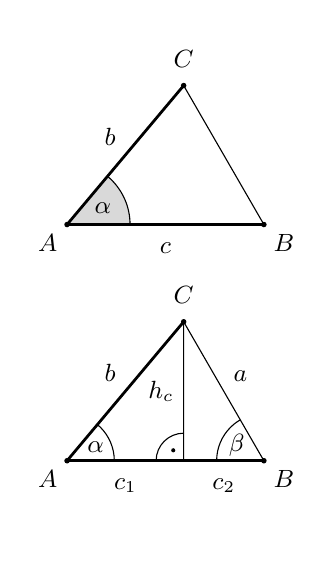
\begin{tikzpicture}[scale=0.5]
    % Zeichenflaeche
    \clip (-1, -8) rectangle (6, 5);
    \begin{scope}
      \coordinate (A) at (0, 0);
      \coordinate (B) at (5, 0);
      \coordinate (C) at (intersection of A--[shift={(50:10)}]A and B--[shift={(120:10)}]B);
      % Winkelflaeche
      \begin{scope}
        \clip (A) -- (B) -- (C) -- cycle;
        \fill[fill=black!15!white] (A) circle (16mm);
      \end{scope}
      % bekannte Seiten
      \draw[line width=1pt] (A) -- (C);
      \draw[line width=1pt] (A) -- (B);
      % Seiten
      \draw (A) -- (B) -- (C) -- cycle;
      % Eckpunkte
      \fill (A) circle (2pt);
      \fill (B) circle (2pt);
      \fill (C) circle (2pt);
      % Winkel
      \begin{scope}
        \clip (A) -- (B) -- (C) -- cycle;
        \draw (A) circle (16mm);
      \end{scope}
      % Beschriftung
      \node[below left]        at (A) {\small$A$};
      \node[below right]       at (B) {\small$B$};
      \node[above=3pt]         at (C) {\small$C$};
      \path (A) -- node[above left]   {\small$b$}(C);
      \path (A) -- node[below=3pt]    {\small$c$}(B);
      \node[shift={(25:5mm)}]  at (A) {\small$\alpha$};
    \end{scope}
    \begin{scope}[yshift=-6cm]
      \coordinate (A) at (0, 0);
      \coordinate (B) at (5, 0);
      \coordinate (C) at (intersection of A--[shift={(50:10)}]A and B--[shift={(120:10)}]B);
      \coordinate (D) at (intersection of A--B and C--[shift={(270:10)}]C);
      % bekannte Seiten
      \draw[line width=1pt] (A) -- (C);
      \draw[line width=1pt] (A) -- (B);
      % Seiten
      \draw (A) -- (B) -- (C) -- cycle;
      % Hoehe
      \draw (C) -- (D);
      % Eckpunkte
      \fill (A) circle (2pt);
      \fill (B) circle (2pt);
      \fill (C) circle (2pt);
      % Winkel
      \begin{scope}
        \clip (A) -- (B) -- (C) -- cycle;
        \draw (A) circle (12mm);
        \draw (B) circle (12mm);
      \end{scope}
      % rechter Winkel
      \begin{scope}
        \clip (A) -- (D) -- (C) -- cycle;
        \draw (D) circle (7mm);
        \fill ([shift={(135:3.75mm)}]D) circle (1.5pt);
      \end{scope}
      % Beschriftung
      \node[below left]        at (A) {\small$A$};
      \node[below right]       at (B) {\small$B$};
      \node[above=3pt]         at (C) {\small$C$};
      \path (A) -- node[above left]   {\small$b$}(C);
      \path (B) -- node[above right]  {\small$a$}(C);
      \path (A) -- node[below=3pt]    {\small$c_{1}$}(D);
      \path (D) -- node[below=3pt]    {\small$c_{2}$}(B);
      \node[shift={(25:4mm)}]  at (A) {\small$\alpha$};
      \node[shift={(150:4mm)}] at (B) {\small$\beta$};
      \path (D) -- node[left]         {\small$h_{c}$}(C);
    \end{scope}
  \end{tikzpicture}%
  \newcommand{\vstrut}{\rule[-2.5ex]{0pt}{6ex}}
  \begin{equation*}
    \begin{split}
       h_{c}\vstrut&=b\cdot\sin\alpha           \\
       c_{1}\vstrut&=b\cdot\cos\alpha           \\
       c_{2}\vstrut&=c-c_{1}                    \\
       \beta\vstrut&=\arctan\frac{h_{c}}{c_{2}} \\
      \gamma\vstrut&=180^{\circ}-\alpha-\beta   \\
           a\vstrut&=\frac{h_{c}}{\sin\beta}
    \end{split}
  \end{equation*}
\end{minipage}\hfill
\begin{minipage}[t]{4cm}
  \centering
  \begingroup
    \usekomafont{sectioning}%
    \usekomafont{paragraph}%
    WSW\bigskip\par
  \endgroup
  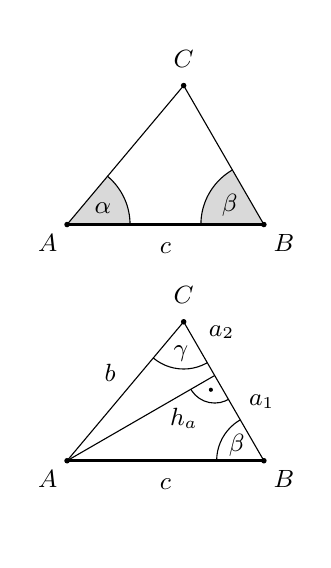
\begin{tikzpicture}[scale=0.5]
    % Zeichenflaeche
    \clip (-1, -8) rectangle (6, 5);
    \begin{scope}
      \coordinate (A) at (0, 0);
      \coordinate (B) at (5, 0);
      \coordinate (C) at (intersection of A--[shift={(50:10)}]A and B--[shift={(120:10)}]B);
      % Winkelflaeche
      \begin{scope}
        \clip (A) -- (B) -- (C) -- cycle;
        \fill[fill=black!15!white] (A) circle (16mm);
        \fill[fill=black!15!white] (B) circle (16mm);
      \end{scope}
      % bekannte Seiten
      \draw[line width=1pt] (A) -- (B);
      % Seiten
      \draw (A) -- (B) -- (C) -- cycle;
      % Eckpunkte
      \fill (A) circle (2pt);
      \fill (B) circle (2pt);
      \fill (C) circle (2pt);
      % Winkel
      \begin{scope}
        \clip (A) -- (B) -- (C) -- cycle;
        \draw (A) circle (16mm);
        \draw (B) circle (16mm);
      \end{scope}
      % Beschriftung
      \node[below left]        at (A) {\small$A$};
      \node[below right]       at (B) {\small$B$};
      \node[above=3pt]         at (C) {\small$C$};
      \path (A) -- node[below=3pt]    {\small$c$}(B);
      \node[shift={(25:5mm)}]  at (A) {\small$\alpha$};
      \node[shift={(150:5mm)}] at (B) {\small$\beta$};
    \end{scope}
    \begin{scope}[yshift=-6cm]
      \coordinate (A) at (0, 0);
      \coordinate (B) at (5, 0);
      \coordinate (C) at (intersection of A--[shift={(50:10)}]A and B--[shift={(120:10)}]B);
      \coordinate (D) at (intersection of A--[shift={(30:10)}]A and B--C);
      % bekannte Seiten
      \draw[line width=1pt] (A) -- (B);
      % Seiten
      \draw (A) -- (B) -- (C) -- cycle;
      % Hoehe
      \draw (A) -- (D);
      % Eckpunkte
      \fill (A) circle (2pt);
      \fill (B) circle (2pt);
      \fill (C) circle (2pt);
      % Winkel
      \begin{scope}
        \clip (A) -- (B) -- (C) -- cycle;
        \draw (B) circle (12mm);
        \draw (C) circle (12mm);
      \end{scope}
      % rechter Winkel
      \begin{scope}
        \clip (A) -- (B) -- (D) -- cycle;
        \draw (D) circle (7mm);
        \fill ([shift={(255:3.75mm)}]D) circle (1.5pt);
      \end{scope}
      % Beschriftung
      \node[below left]        at (A) {\small$A$};
      \node[below right]       at (B) {\small$B$};
      \node[above=3pt]         at (C) {\small$C$};
      \path (A) -- node[below=3pt]    {\small$c$}(B);
      \path (A) -- node[above left]   {\small$b$}(C);
      \path (B) -- node[above right]  {\small$a_{1}$}(D);
      \path (D) -- node[above right]  {\small$a_{2}$}(C);
      \path (A) -- node[right=7pt]    {\small$h_{a}$}(D);
      \node[shift={(150:4mm)}] at (B) {\small$\beta$};
      \node[shift={(265:4mm)}] at (C) {\small$\gamma$};
    \end{scope}
  \end{tikzpicture}%
  \newcommand{\vstrut}{\rule[-2.5ex]{0pt}{6ex}}
  \begin{equation*}
    \begin{split}
       \gamma\vstrut&=180^{\circ}-\alpha-\beta \\
        h_{a}\vstrut&=c\cdot\sin\beta          \\
        a_{1}\vstrut&=c\cdot\cos\beta          \\
        a_{2}\vstrut&=\frac{h_{a}}{\tan\gamma} \\
            a\vstrut&=a_{1}+a_{2}              \\
            b\vstrut&=\frac{h_{a}}{\sin\gamma}
    \end{split}
  \end{equation*}
\end{minipage}\hfill
\begin{minipage}[t]{4cm}
  \centering
  \begingroup
    \usekomafont{sectioning}%
    \usekomafont{paragraph}%
    WWS\bigskip\par
  \endgroup
  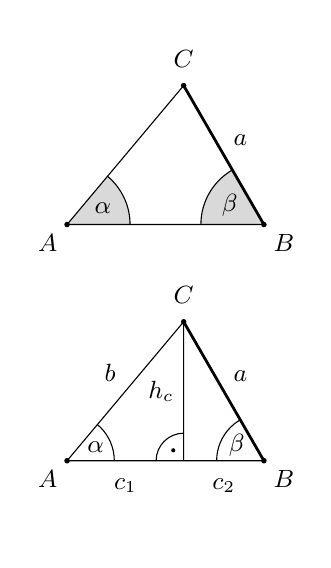
\begin{tikzpicture}[scale=0.5]
    % Zeichenflaeche
    \clip (-1, -8) rectangle (6, 5);
    \begin{scope}
      \coordinate (A) at (0, 0);
      \coordinate (B) at (5, 0);
      \coordinate (C) at (intersection of A--[shift={(50:10)}]A and B--[shift={(120:10)}]B);
      % Winkelflaeche
      \begin{scope}
        \clip (A) -- (B) -- (C) -- cycle;
        \fill[fill=black!15!white] (A) circle (16mm);
        \fill[fill=black!15!white] (B) circle (16mm);
      \end{scope}
      % bekannte Seiten
      \draw[line width=1pt] (B) -- (C);
      % Seiten
      \draw (A) -- (B) -- (C) -- cycle;
      % Eckpunkte
      \fill (A) circle (2pt);
      \fill (B) circle (2pt);
      \fill (C) circle (2pt);
      % Winkel
      \begin{scope}
        \clip (A) -- (B) -- (C) -- cycle;
        \draw (A) circle (16mm);
        \draw (B) circle (16mm);
      \end{scope}
      % Beschriftung
      \node[below left]        at (A) {\small$A$};
      \node[below right]       at (B) {\small$B$};
      \node[above=3pt]         at (C) {\small$C$};
      \path (B) -- node[above right]  {\small$a$}(C);
      \node[shift={(25:5mm)}]  at (A) {\small$\alpha$};
      \node[shift={(150:5mm)}] at (B) {\small$\beta$};
    \end{scope}
    \begin{scope}[yshift=-6cm]
      \coordinate (A) at (0, 0);
      \coordinate (B) at (5, 0);
      \coordinate (C) at (intersection of A--[shift={(50:10)}]A and B--[shift={(120:10)}]B);
      \coordinate (D) at (intersection of A--B and C--[shift={(270:10)}]C);
      % bekannte Seiten
      \draw[line width=1pt] (B) -- (C);
      % Seiten
      \draw (A) -- (B) -- (C) -- cycle;
      % Hoehe
      \draw (C) -- (D);
      % Eckpunkte
      \fill (A) circle (2pt);
      \fill (B) circle (2pt);
      \fill (C) circle (2pt);
      % Winkel
      \begin{scope}
        \clip (A) -- (B) -- (C) -- cycle;
        \draw (A) circle (12mm);
        \draw (B) circle (12mm);
      \end{scope}
      % rechter Winkel
      \begin{scope}
        \clip (A) -- (D) -- (C) -- cycle;
        \draw (D) circle (7mm);
        \fill ([shift={(135:3.75mm)}]D) circle (1.5pt);
      \end{scope}
      % Beschriftung
      \node[below left]        at (A) {\small$A$};
      \node[below right]       at (B) {\small$B$};
      \node[above=3pt]         at (C) {\small$C$};
      \path (A) -- node[above left]   {\small$b$}(C);
      \path (B) -- node[above right]  {\small$a$}(C);
      \path (A) -- node[below=3pt]    {\small$c_{1}$}(D);
      \path (D) -- node[below=3pt]    {\small$c_{2}$}(B);
      \path (D) -- node[left]         {\small$h_{c}$}(C);
      \node[shift={(25:4mm)}]  at (A) {\small$\alpha$};
      \node[shift={(150:4mm)}] at (B) {\small$\beta$};
    \end{scope}
  \end{tikzpicture}%
  \newcommand{\vstrut}{\rule[-2.5ex]{0pt}{6ex}}
  \begin{equation*}
    \begin{split}
       \gamma\vstrut&=180^{\circ}-\alpha-\beta \\
        h_{c}\vstrut&=a\cdot\sin\beta          \\
        c_{2}\vstrut&=a\cdot\cos\beta          \\
            b\vstrut&=\frac{h_{c}}{\sin\alpha} \\
        c_{1}\vstrut&=b\cdot\cos\alpha         \\
            c\vstrut&=c_{1}+c_{2}
    \end{split}
  \end{equation*}
\end{minipage}\hfill
\begin{minipage}[t]{4cm}
  \centering
  \begingroup
    \usekomafont{sectioning}%
    \usekomafont{paragraph}%
    SsW\bigskip\par
  \endgroup
  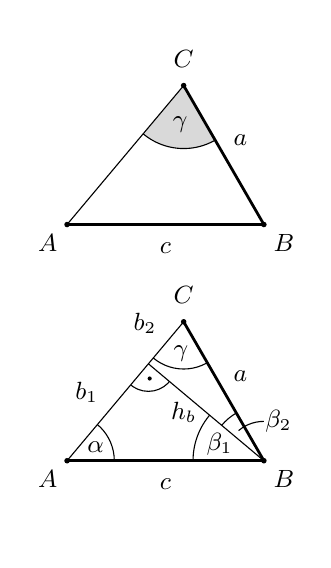
\begin{tikzpicture}[scale=0.5]
    % Zeichenflaeche
    \clip (-1, -8) rectangle (6, 5);
    \begin{scope}
      \coordinate (A) at (0, 0);
      \coordinate (B) at (5, 0);
      \coordinate (C) at (intersection of A--[shift={(50:10)}]A and B--[shift={(120:10)}]B);
      % Winkelflaeche
      \begin{scope}
        \clip (A) -- (B) -- (C) -- cycle;
        \fill[fill=black!15!white] (C) circle (16mm);
      \end{scope}
      % bekannte Seiten
      \draw[line width=1pt] (A) -- (B);
      \draw[line width=1pt] (B) -- (C);
      % Seiten
      \draw (A) -- (B) -- (C) -- cycle;
      % Eckpunkte
      \fill (A) circle (2pt);
      \fill (B) circle (2pt);
      \fill (C) circle (2pt);
      % Winkel
      \begin{scope}
        \clip (A) -- (B) -- (C) -- cycle;
        \draw (C) circle (16mm);
      \end{scope}
      % Beschriftung
      \node[below left]        at (A) {\small$A$};
      \node[below right]       at (B) {\small$B$};
      \node[above=3pt]         at (C) {\small$C$};
      \path (A) -- node[below=3pt]    {\small$c$}(B);
      \path (B) -- node[above right]  {\small$a$}(C);
      \node[shift={(265:5mm)}] at (C) {\small$\gamma$};
    \end{scope}
    \begin{scope}[yshift=-6cm]
      \coordinate (A) at (0, 0);
      \coordinate (B) at (5, 0);
      \coordinate (C) at (intersection of A--[shift={(50:10)}]A and B--[shift={(120:10)}]B);
      \coordinate (D) at (intersection of B--[shift={(140:10)}]B and A--C);
      % bekannte Seiten
      \draw[line width=1pt] (A) -- (B);
      \draw[line width=1pt] (B) -- (C);
      % Seiten
      \draw (A) -- (B) -- (C) -- cycle;
      % Hoehe
      \draw (B) -- (D);
      % Eckpunkte
      \fill (A) circle (2pt);
      \fill (B) circle (2pt);
      \fill (C) circle (2pt);
      % Winkel
      \begin{scope}
        \clip (A) -- (B) -- (C) -- cycle;
        \draw (A) circle (12mm);
        \draw (C) circle (12mm);
      \end{scope}
      % Winkel beta 1
      \begin{scope}
        \clip (A) -- (B) -- (D) -- cycle;
        \draw (B) circle (18mm);
      \end{scope}
      % Winkel beta 2
      \begin{scope}
        \clip (B) -- (C) -- (D) -- cycle;
        \draw (B) circle (14mm);
      \end{scope}
      % rechter Winkel
      \begin{scope}
        \clip (A) -- (B) -- (D) -- cycle;
        \draw (D) circle (7mm);
        \fill ([shift={(275:3.75mm)}]D) circle (1.5pt);
      \end{scope}
      % Strich zwischen beta 2 und dem Winkel
      \begin{scope}
        \clip (B) -- +(130:50mm) -- +(90:50mm) -- cycle;
        \draw (B) circle (10mm);
      \end{scope}
      % Beschriftung
      \node[below left]         at (A) {\small$A$};
      \node[below right]        at (B) {\small$B$};
      \node[above=3pt]          at (C) {\small$C$};
      \path (B) -- node[above right]   {\small$a$}(C);
      \path (A) -- node[below=3pt]     {\small$c$}(B);
      \path (A) -- node[above left]    {\small$b_{1}$}(D);
      \path (D) -- node[above left]    {\small$b_{2}$}(C);
      \path (B) -- node[left]          {\small$h_{b}$}(D);
      \node[shift={(25:4mm)}]   at (A) {\small$\alpha$};
      \node[shift={(160:6mm)}]  at (B) {\small$\beta_{1}$};
      \path (B) -- +(90:10mm) node[right=-3pt] {{\small$\beta_{2}$}};
      \node[shift={(265:4mm)}]  at (C) {\small$\gamma$};
    \end{scope}
  \end{tikzpicture}%
  \newcommand{\vstrut}{\rule[-2.5ex]{0pt}{6ex}}
  \begin{equation*}
    \begin{split}
        h_{b}\vstrut&=a\cdot\sin\gamma         \\
        b_{2}\vstrut&=a\cdot\cos\gamma         \\
       \alpha\vstrut&=\arcsin\frac{h_{b}}{c}   \\
        b_{1}\vstrut&=c\cdot\cos\alpha         \\
            b\vstrut&=b_{1}+b_{2}              \\
        \beta\vstrut&=180^{\circ}-\alpha-\gamma
    \end{split}
  \end{equation*}
\end{minipage}\vspace{2.5\baselineskip}

\begin{minipage}[t]{4cm}
  \centering
  \begingroup
    \usekomafont{sectioning}%
    \usekomafont{paragraph}%
    SSS\bigskip\par
  \endgroup
  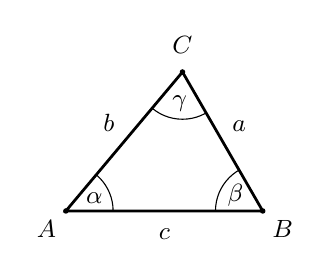
\begin{tikzpicture}[scale=0.5]
    \begin{scope}
      \coordinate (A) at (0, 0);
      \coordinate (B) at (5, 0);
      \coordinate (C) at (intersection of A--[shift={(50:10)}]A and B--[shift={(120:10)}]B);
      % bekannte Seiten
      \draw[line width=1pt] (A) -- (B) -- (C) -- cycle;
      % Eckpunkte
      \fill (A) circle (2pt);
      \fill (B) circle (2pt);
      \fill (C) circle (2pt);
      % Winkel
      \begin{scope}
        \clip (A) -- (B) -- (C) -- cycle;
        \draw (A) circle (12mm);
        \draw (B) circle (12mm);
        \draw (C) circle (12mm);
      \end{scope}
      % Beschriftung
      \node[below left]        at (A) {\small$A$};
      \node[below right]       at (B) {\small$B$};
      \node[above=3pt]         at (C) {\small$C$};
      \path (B) -- node[above right]  {\small$a$}(C);
      \path (A) -- node[above left]   {\small$b$}(C);
      \path (A) -- node[below=3pt]    {\small$c$}(B);
      \node[shift={(25:4mm)}]  at (A) {\small$\alpha$};
      \node[shift={(150:4mm)}] at (B) {\small$\beta$};
      \node[shift={(265:4mm)}] at (C) {\small$\gamma$};
    \end{scope}
  \end{tikzpicture}%
\end{minipage}%
\begin{minipage}[t]{5cm}
  \newcommand{\vstrut}{\rule[-3ex]{0pt}{7ex}}
  \begin{equation*}
    \begin{split}
      \alpha\vstrut&=\arccos\frac{b^{2}+c^{2}-a^{2}}{2bc} \\
       \beta\vstrut&=\arccos\frac{a^{2}+c^{2}-b^{2}}{2ac} \\
      \gamma\vstrut&=\arccos\frac{a^{2}+b^{2}-c^{2}}{2ab}
    \end{split}
  \end{equation*}%
\end{minipage}


\newpage
% -----------------------
\mysec{Großes Einmaleins}
% -----------------------
\begin{center}
  \renewcommand{\arraystretch}{1.33}%
  \newcommand{\q}[1]{{\bfseries#1}}%
  \rotatebox{90}{%
  \begin{tabular}{c|rrrrrrrrr|c|rrrrrrrrrr|c}
         &    2    &    3    &    4    &    5    &    6    &    7    &    8    &    9    &    10    &         &    11    &    12    &   13    &    14    &    15    &   16    &    17    &    18    &    19    &    20    &        \\
  \hline
    2    &\q{4}    &    6    &    8    &   10    &   12    &   14    &   16    &   18    &    20    &    2    &    22    &    24    &   26    &    28    &    30    &   32    &    34    &    36    &    38    &    40    &    2   \\
    3    &    6    & \q{9}   &   12    &   15    &   18    &   21    &   24    &   27    &    30    &    3    &    33    &    36    &   39    &    42    &    45    &   48    &    51    &    54    &    57    &    60    &    3   \\
    4    &    8    &   12    &\q{16}   &   20    &   24    &   28    &   32    &   36    &    40    &    4    &    44    &    48    &   52    &    56    &    60    &   64    &    68    &    72    &    76    &    80    &    4   \\
    5    &   10    &   15    &   20    &\q{25}   &   30    &   35    &   40    &   45    &    50    &    5    &    55    &    60    &   65    &    70    &    75    &   80    &    85    &    90    &    95    &   100    &    5   \\
    6    &   12    &   18    &   24    &   30    &\q{36}   &   42    &   48    &   54    &    60    &    6    &    66    &    72    &   78    &    84    &    90    &   96    &   102    &   108    &   114    &   120    &    6   \\
    7    &   14    &   21    &   28    &   35    &   42    &\q{49}   &   56    &   63    &    70    &    7    &    77    &    84    &   91    &    98    &   105    &  112    &   119    &   126    &   133    &   140    &    7   \\
    8    &   16    &   24    &   32    &   40    &   48    &   56    &\q{64}   &   72    &    80    &    8    &    88    &    96    &  104    &   112    &   120    &  128    &   136    &   144    &   152    &   160    &    8   \\
    9    &   18    &   27    &   36    &   45    &   54    &   63    &   72    &\q{81}   &    90    &    9    &    99    &   108    &  117    &   126    &   135    &  144    &   153    &   162    &   171    &   180    &    9   \\
   10    &   20    &   30    &   40    &   50    &   60    &   70    &   80    &   90    &\q{100}   &   10    &   110    &   120    &  130    &   140    &   150    &  160    &   170    &   180    &   190    &   200    &   10   \\
  \hline
         &    2    &    3    &    4    &    5    &    6    &    7    &    8    &    9    &    10    &         &    11    &    12    &   13    &    14    &    15    &   16    &    17    &    18    &    19    &    20    &        \\
  \hline
   11    &   22    &   33    &   44    &   55    &   66    &   77    &   88    &   99    &   110    &   11    &\q{121}   &   132    &  143    &   154    &   165    &  176    &   187    &   198    &   209    &   220    &   11   \\
   12    &   24    &   36    &   48    &   60    &   72    &   84    &   96    &  108    &   120    &   12    &   132    &\q{144}   &  156    &   168    &   180    &  192    &   204    &   216    &   228    &   240    &   12   \\
   13    &   26    &   39    &   52    &   65    &   78    &   91    &  104    &  117    &   130    &   13    &   143    &   156    &\q{169}  &   182    &   195    &  208    &   221    &   234    &   247    &   260    &   13   \\
   14    &   28    &   42    &   56    &   70    &   84    &   98    &  112    &  126    &   140    &   14    &   154    &   168    &  182    &\q{196}   &   210    &  224    &   238    &   252    &   266    &   280    &   14   \\
   15    &   30    &   45    &   60    &   75    &   90    &  105    &  120    &  135    &   150    &   15    &   165    &   180    &  195    &   210    &\q{225}   &  240    &   255    &   270    &   285    &   300    &   15   \\
   16    &   32    &   48    &   64    &   80    &   96    &  112    &  128    &  144    &   160    &   16    &   176    &   192    &  208    &   224    &   240    &\q{256}  &   272    &   288    &   304    &   320    &   16   \\
   17    &   34    &   51    &   68    &   85    &  102    &  119    &  136    &  153    &   170    &   17    &   187    &   204    &  221    &   238    &   255    &  272    &\q{289}   &   306    &   323    &   340    &   17   \\
   18    &   36    &   54    &   72    &   90    &  108    &  126    &  144    &  162    &   180    &   18    &   198    &   216    &  234    &   252    &   270    &  288    &   306    &\q{324}   &   342    &   360    &   18   \\
   19    &   38    &   57    &   76    &   95    &  114    &  133    &  152    &  171    &   190    &   19    &   209    &   228    &  247    &   266    &   285    &  304    &   323    &   342    &\q{361}   &   380    &   19   \\
   20    &   40    &   60    &   80    &  100    &  120    &  140    &  160    &  180    &   200    &   20    &   220    &   240    &  260    &   280    &   300    &  320    &   340    &   360    &   380    &\q{400}   &   20   \\
  \hline
         &    2    &    3    &    4    &    5    &    6    &    7    &    8    &    9    &    10    &         &    11    &    12    &   13    &    14    &    15    &   16    &    17    &    18    &    19    &    20    &        \\
  \end{tabular}}
\end{center}

\newpage
% ---------------------
\mysec{Viertelquadrate}
% ---------------------
\begin{center}
  \begin{minipage}[c]{4cm}
    \centering
    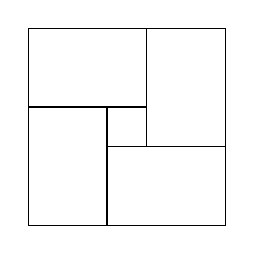
\begin{tikzpicture}[scale=0.50]
      \draw (0, 0) rectangle (5, 5);
      \draw (2, 0) -- (2, 3);
      \draw (5, 2) -- (2, 2);
      \draw (3, 5) -- (3, 2);
      \draw (0, 3) -- (3, 3);
    \end{tikzpicture}
  \end{minipage}
  \begin{minipage}[c]{14em}
    \vspace*{-\abovedisplayskip}
    \begin{equation*}
      \begin{split}
        4\cdot ab&=(a+b)^{2}-(a-b)^{2}\\[2ex]
        \Rightarrow\quad ab&=\frac{(a+b)^{2}-(a-b)^{2}}{4}
      \end{split}
    \end{equation*}
  \end{minipage}
\end{center}
\vfill
\begin{center}\small
\makebox[4em][r]{~}%
\makebox[4em][r]{0}%
\makebox[4em][r]{1}%
\makebox[4em][r]{2}%
\makebox[4em][r]{3}%
\makebox[4em][r]{4}%
\makebox[4em][r]{5}%
\makebox[4em][r]{6}%
\makebox[4em][r]{7}%
\makebox[4em][r]{8}%
\makebox[4em][r]{9}\\[1ex]
\makebox[4em][r]{0}%
\makebox[4em][r]{0}%
\makebox[4em][r]{0}%
\makebox[4em][r]{1}%
\makebox[4em][r]{2}%
\makebox[4em][r]{4}%
\makebox[4em][r]{6}%
\makebox[4em][r]{9}%
\makebox[4em][r]{12}%
\makebox[4em][r]{16}%
\makebox[4em][r]{20}\\
\makebox[4em][r]{10}%
\makebox[4em][r]{25}%
\makebox[4em][r]{30}%
\makebox[4em][r]{36}%
\makebox[4em][r]{42}%
\makebox[4em][r]{49}%
\makebox[4em][r]{56}%
\makebox[4em][r]{64}%
\makebox[4em][r]{72}%
\makebox[4em][r]{81}%
\makebox[4em][r]{90}\\
\makebox[4em][r]{20}%
\makebox[4em][r]{100}%
\makebox[4em][r]{110}%
\makebox[4em][r]{121}%
\makebox[4em][r]{132}%
\makebox[4em][r]{144}%
\makebox[4em][r]{156}%
\makebox[4em][r]{169}%
\makebox[4em][r]{182}%
\makebox[4em][r]{196}%
\makebox[4em][r]{210}\\
\makebox[4em][r]{30}%
\makebox[4em][r]{225}%
\makebox[4em][r]{240}%
\makebox[4em][r]{256}%
\makebox[4em][r]{272}%
\makebox[4em][r]{289}%
\makebox[4em][r]{306}%
\makebox[4em][r]{324}%
\makebox[4em][r]{342}%
\makebox[4em][r]{361}%
\makebox[4em][r]{380}\\
\makebox[4em][r]{40}%
\makebox[4em][r]{400}%
\makebox[4em][r]{420}%
\makebox[4em][r]{441}%
\makebox[4em][r]{462}%
\makebox[4em][r]{484}%
\makebox[4em][r]{506}%
\makebox[4em][r]{529}%
\makebox[4em][r]{552}%
\makebox[4em][r]{576}%
\makebox[4em][r]{600}\\
\makebox[4em][r]{50}%
\makebox[4em][r]{625}%
\makebox[4em][r]{650}%
\makebox[4em][r]{676}%
\makebox[4em][r]{702}%
\makebox[4em][r]{729}%
\makebox[4em][r]{756}%
\makebox[4em][r]{784}%
\makebox[4em][r]{812}%
\makebox[4em][r]{841}%
\makebox[4em][r]{870}\\
\makebox[4em][r]{60}%
\makebox[4em][r]{900}%
\makebox[4em][r]{930}%
\makebox[4em][r]{961}%
\makebox[4em][r]{992}%
\makebox[4em][r]{1024}%
\makebox[4em][r]{1056}%
\makebox[4em][r]{1089}%
\makebox[4em][r]{1122}%
\makebox[4em][r]{1156}%
\makebox[4em][r]{1190}\\
\makebox[4em][r]{70}%
\makebox[4em][r]{1225}%
\makebox[4em][r]{1260}%
\makebox[4em][r]{1296}%
\makebox[4em][r]{1332}%
\makebox[4em][r]{1369}%
\makebox[4em][r]{1406}%
\makebox[4em][r]{1444}%
\makebox[4em][r]{1482}%
\makebox[4em][r]{1521}%
\makebox[4em][r]{1560}\\
\makebox[4em][r]{80}%
\makebox[4em][r]{1600}%
\makebox[4em][r]{1640}%
\makebox[4em][r]{1681}%
\makebox[4em][r]{1722}%
\makebox[4em][r]{1764}%
\makebox[4em][r]{1806}%
\makebox[4em][r]{1849}%
\makebox[4em][r]{1892}%
\makebox[4em][r]{1936}%
\makebox[4em][r]{1980}\\
\makebox[4em][r]{90}%
\makebox[4em][r]{2025}%
\makebox[4em][r]{2070}%
\makebox[4em][r]{2116}%
\makebox[4em][r]{2162}%
\makebox[4em][r]{2209}%
\makebox[4em][r]{2256}%
\makebox[4em][r]{2304}%
\makebox[4em][r]{2352}%
\makebox[4em][r]{2401}%
\makebox[4em][r]{2450}\\
\makebox[4em][r]{100}%
\makebox[4em][r]{2500}%
\makebox[4em][r]{2550}%
\makebox[4em][r]{2601}%
\makebox[4em][r]{2652}%
\makebox[4em][r]{2704}%
\makebox[4em][r]{2756}%
\makebox[4em][r]{2809}%
\makebox[4em][r]{2862}%
\makebox[4em][r]{2916}%
\makebox[4em][r]{2970}\\
\makebox[4em][r]{110}%
\makebox[4em][r]{3025}%
\makebox[4em][r]{3080}%
\makebox[4em][r]{3136}%
\makebox[4em][r]{3192}%
\makebox[4em][r]{3249}%
\makebox[4em][r]{3306}%
\makebox[4em][r]{3364}%
\makebox[4em][r]{3422}%
\makebox[4em][r]{3481}%
\makebox[4em][r]{3540}\\
\makebox[4em][r]{120}%
\makebox[4em][r]{3600}%
\makebox[4em][r]{3660}%
\makebox[4em][r]{3721}%
\makebox[4em][r]{3782}%
\makebox[4em][r]{3844}%
\makebox[4em][r]{3906}%
\makebox[4em][r]{3969}%
\makebox[4em][r]{4032}%
\makebox[4em][r]{4096}%
\makebox[4em][r]{4160}\\
\makebox[4em][r]{130}%
\makebox[4em][r]{4225}%
\makebox[4em][r]{4290}%
\makebox[4em][r]{4356}%
\makebox[4em][r]{4422}%
\makebox[4em][r]{4489}%
\makebox[4em][r]{4556}%
\makebox[4em][r]{4624}%
\makebox[4em][r]{4692}%
\makebox[4em][r]{4761}%
\makebox[4em][r]{4830}\\
\makebox[4em][r]{140}%
\makebox[4em][r]{4900}%
\makebox[4em][r]{4970}%
\makebox[4em][r]{5041}%
\makebox[4em][r]{5112}%
\makebox[4em][r]{5184}%
\makebox[4em][r]{5256}%
\makebox[4em][r]{5329}%
\makebox[4em][r]{5402}%
\makebox[4em][r]{5476}%
\makebox[4em][r]{5550}\\
\makebox[4em][r]{150}%
\makebox[4em][r]{5625}%
\makebox[4em][r]{5700}%
\makebox[4em][r]{5776}%
\makebox[4em][r]{5852}%
\makebox[4em][r]{5929}%
\makebox[4em][r]{6006}%
\makebox[4em][r]{6084}%
\makebox[4em][r]{6162}%
\makebox[4em][r]{6241}%
\makebox[4em][r]{6320}\\
\makebox[4em][r]{160}%
\makebox[4em][r]{6400}%
\makebox[4em][r]{6480}%
\makebox[4em][r]{6561}%
\makebox[4em][r]{6642}%
\makebox[4em][r]{6724}%
\makebox[4em][r]{6806}%
\makebox[4em][r]{6889}%
\makebox[4em][r]{6972}%
\makebox[4em][r]{7056}%
\makebox[4em][r]{7140}\\
\makebox[4em][r]{170}%
\makebox[4em][r]{7225}%
\makebox[4em][r]{7310}%
\makebox[4em][r]{7396}%
\makebox[4em][r]{7482}%
\makebox[4em][r]{7569}%
\makebox[4em][r]{7656}%
\makebox[4em][r]{7744}%
\makebox[4em][r]{7832}%
\makebox[4em][r]{7921}%
\makebox[4em][r]{8010}\\
\makebox[4em][r]{180}%
\makebox[4em][r]{8100}%
\makebox[4em][r]{8190}%
\makebox[4em][r]{8281}%
\makebox[4em][r]{8372}%
\makebox[4em][r]{8464}%
\makebox[4em][r]{8556}%
\makebox[4em][r]{8649}%
\makebox[4em][r]{8742}%
\makebox[4em][r]{8836}%
\makebox[4em][r]{8930}\\
\makebox[4em][r]{190}%
\makebox[4em][r]{9025}%
\makebox[4em][r]{9120}%
\makebox[4em][r]{9216}%
\makebox[4em][r]{9312}%
\makebox[4em][r]{9409}%
\makebox[4em][r]{9506}%
\makebox[4em][r]{9604}%
\makebox[4em][r]{9702}%
\makebox[4em][r]{9801}%
\makebox[4em][r]{9900}\\
\makebox[4em][r]{200}%
\makebox[4em][r]{10000}%
\makebox[4em][r]{10100}%
\makebox[4em][r]{10201}%
\makebox[4em][r]{10302}%
\makebox[4em][r]{10404}%
\makebox[4em][r]{10506}%
\makebox[4em][r]{10609}%
\makebox[4em][r]{10712}%
\makebox[4em][r]{10816}%
\makebox[4em][r]{10920}\\
\makebox[4em][r]{210}%
\makebox[4em][r]{11025}%
\makebox[4em][r]{11130}%
\makebox[4em][r]{11236}%
\makebox[4em][r]{11342}%
\makebox[4em][r]{11449}%
\makebox[4em][r]{11556}%
\makebox[4em][r]{11664}%
\makebox[4em][r]{11772}%
\makebox[4em][r]{11881}%
\makebox[4em][r]{11990}\\
\makebox[4em][r]{220}%
\makebox[4em][r]{12100}%
\makebox[4em][r]{12210}%
\makebox[4em][r]{12321}%
\makebox[4em][r]{12432}%
\makebox[4em][r]{12544}%
\makebox[4em][r]{12656}%
\makebox[4em][r]{12769}%
\makebox[4em][r]{12882}%
\makebox[4em][r]{12996}%
\makebox[4em][r]{13110}\\
\makebox[4em][r]{230}%
\makebox[4em][r]{13225}%
\makebox[4em][r]{13340}%
\makebox[4em][r]{13456}%
\makebox[4em][r]{13572}%
\makebox[4em][r]{13689}%
\makebox[4em][r]{13806}%
\makebox[4em][r]{13924}%
\makebox[4em][r]{14042}%
\makebox[4em][r]{14161}%
\makebox[4em][r]{14280}\\
\makebox[4em][r]{240}%
\makebox[4em][r]{14400}%
\makebox[4em][r]{14520}%
\makebox[4em][r]{14641}%
\makebox[4em][r]{14762}%
\makebox[4em][r]{14884}%
\makebox[4em][r]{15006}%
\makebox[4em][r]{15129}%
\makebox[4em][r]{15252}%
\makebox[4em][r]{15376}%
\makebox[4em][r]{15500}\\
\makebox[4em][r]{250}%
\makebox[4em][r]{15625}%
\makebox[4em][r]{15750}%
\makebox[4em][r]{15876}%
\makebox[4em][r]{16002}%
\makebox[4em][r]{16129}%
\makebox[4em][r]{16256}%
\makebox[4em][r]{16384}%
\makebox[4em][r]{16512}%
\makebox[4em][r]{16641}%
\makebox[4em][r]{16770}\\
\makebox[4em][r]{260}%
\makebox[4em][r]{16900}%
\makebox[4em][r]{17030}%
\makebox[4em][r]{17161}%
\makebox[4em][r]{17292}%
\makebox[4em][r]{17424}%
\makebox[4em][r]{17556}%
\makebox[4em][r]{17689}%
\makebox[4em][r]{17822}%
\makebox[4em][r]{17956}%
\makebox[4em][r]{18090}\\
\makebox[4em][r]{270}%
\makebox[4em][r]{18225}%
\makebox[4em][r]{18360}%
\makebox[4em][r]{18496}%
\makebox[4em][r]{18632}%
\makebox[4em][r]{18769}%
\makebox[4em][r]{18906}%
\makebox[4em][r]{19044}%
\makebox[4em][r]{19182}%
\makebox[4em][r]{19321}%
\makebox[4em][r]{19460}\\
\makebox[4em][r]{280}%
\makebox[4em][r]{19600}%
\makebox[4em][r]{19740}%
\makebox[4em][r]{19881}%
\makebox[4em][r]{20022}%
\makebox[4em][r]{20164}%
\makebox[4em][r]{20306}%
\makebox[4em][r]{20449}%
\makebox[4em][r]{20592}%
\makebox[4em][r]{20736}%
\makebox[4em][r]{20880}\\
\makebox[4em][r]{290}%
\makebox[4em][r]{21025}%
\makebox[4em][r]{21170}%
\makebox[4em][r]{21316}%
\makebox[4em][r]{21462}%
\makebox[4em][r]{21609}%
\makebox[4em][r]{21756}%
\makebox[4em][r]{21904}%
\makebox[4em][r]{22052}%
\makebox[4em][r]{22201}%
\makebox[4em][r]{22350}\\
\makebox[4em][r]{300}%
\makebox[4em][r]{22500}%
\makebox[4em][r]{22650}%
\makebox[4em][r]{22801}%
\makebox[4em][r]{22952}%
\makebox[4em][r]{23104}%
\makebox[4em][r]{23256}%
\makebox[4em][r]{23409}%
\makebox[4em][r]{23562}%
\makebox[4em][r]{23716}%
\makebox[4em][r]{23870}\\
\makebox[4em][r]{310}%
\makebox[4em][r]{24025}%
\makebox[4em][r]{24180}%
\makebox[4em][r]{24336}%
\makebox[4em][r]{24492}%
\makebox[4em][r]{24649}%
\makebox[4em][r]{24806}%
\makebox[4em][r]{24964}%
\makebox[4em][r]{25122}%
\makebox[4em][r]{25281}%
\makebox[4em][r]{25440}\\
\makebox[4em][r]{320}%
\makebox[4em][r]{25600}%
\makebox[4em][r]{25760}%
\makebox[4em][r]{25921}%
\makebox[4em][r]{26082}%
\makebox[4em][r]{26244}%
\makebox[4em][r]{26406}%
\makebox[4em][r]{26569}%
\makebox[4em][r]{26732}%
\makebox[4em][r]{26896}%
\makebox[4em][r]{27060}\\
\makebox[4em][r]{330}%
\makebox[4em][r]{27225}%
\makebox[4em][r]{27390}%
\makebox[4em][r]{27556}%
\makebox[4em][r]{27722}%
\makebox[4em][r]{27889}%
\makebox[4em][r]{28056}%
\makebox[4em][r]{28224}%
\makebox[4em][r]{28392}%
\makebox[4em][r]{28561}%
\makebox[4em][r]{28730}\\
\makebox[4em][r]{340}%
\makebox[4em][r]{28900}%
\makebox[4em][r]{29070}%
\makebox[4em][r]{29241}%
\makebox[4em][r]{29412}%
\makebox[4em][r]{29584}%
\makebox[4em][r]{29756}%
\makebox[4em][r]{29929}%
\makebox[4em][r]{30102}%
\makebox[4em][r]{30276}%
\makebox[4em][r]{30450}\\
\makebox[4em][r]{350}%
\makebox[4em][r]{30625}%
\makebox[4em][r]{30800}%
\makebox[4em][r]{30976}%
\makebox[4em][r]{31152}%
\makebox[4em][r]{31329}%
\makebox[4em][r]{31506}%
\makebox[4em][r]{31684}%
\makebox[4em][r]{31862}%
\makebox[4em][r]{32041}%
\makebox[4em][r]{32220}\\
\makebox[4em][r]{360}%
\makebox[4em][r]{32400}%
\makebox[4em][r]{32580}%
\makebox[4em][r]{32761}%
\makebox[4em][r]{32942}%
\makebox[4em][r]{33124}%
\makebox[4em][r]{33306}%
\makebox[4em][r]{33489}%
\makebox[4em][r]{33672}%
\makebox[4em][r]{33856}%
\makebox[4em][r]{34040}\\
\makebox[4em][r]{370}%
\makebox[4em][r]{34225}%
\makebox[4em][r]{34410}%
\makebox[4em][r]{34596}%
\makebox[4em][r]{34782}%
\makebox[4em][r]{34969}%
\makebox[4em][r]{35156}%
\makebox[4em][r]{35344}%
\makebox[4em][r]{35532}%
\makebox[4em][r]{35721}%
\makebox[4em][r]{35910}\\
\makebox[4em][r]{380}%
\makebox[4em][r]{36100}%
\makebox[4em][r]{36290}%
\makebox[4em][r]{36481}%
\makebox[4em][r]{36672}%
\makebox[4em][r]{36864}%
\makebox[4em][r]{37056}%
\makebox[4em][r]{37249}%
\makebox[4em][r]{37442}%
\makebox[4em][r]{37636}%
\makebox[4em][r]{37830}\\
\makebox[4em][r]{390}%
\makebox[4em][r]{38025}%
\makebox[4em][r]{38220}%
\makebox[4em][r]{38416}%
\makebox[4em][r]{38612}%
\makebox[4em][r]{38809}%
\makebox[4em][r]{39006}%
\makebox[4em][r]{39204}%
\makebox[4em][r]{39402}%
\makebox[4em][r]{39601}%
\makebox[4em][r]{39800}\\
\makebox[4em][r]{400}%
\makebox[4em][r]{40000}%
\makebox[4em][r]{40200}%
\makebox[4em][r]{40401}%
\makebox[4em][r]{40602}%
\makebox[4em][r]{40804}%
\makebox[4em][r]{41006}%
\makebox[4em][r]{41209}%
\makebox[4em][r]{41412}%
\makebox[4em][r]{41616}%
\makebox[4em][r]{41820}\\
\makebox[4em][r]{410}%
\makebox[4em][r]{42025}%
\makebox[4em][r]{42230}%
\makebox[4em][r]{42436}%
\makebox[4em][r]{42642}%
\makebox[4em][r]{42849}%
\makebox[4em][r]{43056}%
\makebox[4em][r]{43264}%
\makebox[4em][r]{43472}%
\makebox[4em][r]{43681}%
\makebox[4em][r]{43890}\\
\makebox[4em][r]{420}%
\makebox[4em][r]{44100}%
\makebox[4em][r]{44310}%
\makebox[4em][r]{44521}%
\makebox[4em][r]{44732}%
\makebox[4em][r]{44944}%
\makebox[4em][r]{45156}%
\makebox[4em][r]{45369}%
\makebox[4em][r]{45582}%
\makebox[4em][r]{45796}%
\makebox[4em][r]{46010}%
\end{center}

\newpage
% ----------------
\mysec{Primzahlen}
% ----------------
\begin{center}\small
\makebox[2.9em][r]{2}%
\makebox[2.9em][r]{251}%
\makebox[2.9em][r]{587}%
\makebox[2.9em][r]{941}%
\makebox[2.9em][r]{1303}%
\makebox[2.9em][r]{1699}%
\makebox[2.9em][r]{2113}%
\makebox[2.9em][r]{2543}%
\makebox[2.9em][r]{2953}%
\makebox[2.9em][r]{3391}%
\makebox[2.9em][r]{3823}%
\makebox[2.9em][r]{4259}%
\makebox[2.9em][r]{4723}%
\makebox[2.9em][r]{5179}%
\makebox[2.9em][r]{5651}%
\makebox[2.9em][r]{6101}\\
\makebox[2.9em][r]{3}%
\makebox[2.9em][r]{257}%
\makebox[2.9em][r]{593}%
\makebox[2.9em][r]{947}%
\makebox[2.9em][r]{1307}%
\makebox[2.9em][r]{1709}%
\makebox[2.9em][r]{2129}%
\makebox[2.9em][r]{2549}%
\makebox[2.9em][r]{2957}%
\makebox[2.9em][r]{3407}%
\makebox[2.9em][r]{3833}%
\makebox[2.9em][r]{4261}%
\makebox[2.9em][r]{4729}%
\makebox[2.9em][r]{5189}%
\makebox[2.9em][r]{5653}%
\makebox[2.9em][r]{6113}\\
\makebox[2.9em][r]{5}%
\makebox[2.9em][r]{263}%
\makebox[2.9em][r]{599}%
\makebox[2.9em][r]{953}%
\makebox[2.9em][r]{1319}%
\makebox[2.9em][r]{1721}%
\makebox[2.9em][r]{2131}%
\makebox[2.9em][r]{2551}%
\makebox[2.9em][r]{2963}%
\makebox[2.9em][r]{3413}%
\makebox[2.9em][r]{3847}%
\makebox[2.9em][r]{4271}%
\makebox[2.9em][r]{4733}%
\makebox[2.9em][r]{5197}%
\makebox[2.9em][r]{5657}%
\makebox[2.9em][r]{6121}\\
\makebox[2.9em][r]{7}%
\makebox[2.9em][r]{269}%
\makebox[2.9em][r]{601}%
\makebox[2.9em][r]{967}%
\makebox[2.9em][r]{1321}%
\makebox[2.9em][r]{1723}%
\makebox[2.9em][r]{2137}%
\makebox[2.9em][r]{2557}%
\makebox[2.9em][r]{2969}%
\makebox[2.9em][r]{3433}%
\makebox[2.9em][r]{3851}%
\makebox[2.9em][r]{4273}%
\makebox[2.9em][r]{4751}%
\makebox[2.9em][r]{5209}%
\makebox[2.9em][r]{5659}%
\makebox[2.9em][r]{6131}\\
\makebox[2.9em][r]{11}%
\makebox[2.9em][r]{271}%
\makebox[2.9em][r]{607}%
\makebox[2.9em][r]{971}%
\makebox[2.9em][r]{1327}%
\makebox[2.9em][r]{1733}%
\makebox[2.9em][r]{2141}%
\makebox[2.9em][r]{2579}%
\makebox[2.9em][r]{2971}%
\makebox[2.9em][r]{3449}%
\makebox[2.9em][r]{3853}%
\makebox[2.9em][r]{4283}%
\makebox[2.9em][r]{4759}%
\makebox[2.9em][r]{5227}%
\makebox[2.9em][r]{5669}%
\makebox[2.9em][r]{6133}\\
\makebox[2.9em][r]{13}%
\makebox[2.9em][r]{277}%
\makebox[2.9em][r]{613}%
\makebox[2.9em][r]{977}%
\makebox[2.9em][r]{1361}%
\makebox[2.9em][r]{1741}%
\makebox[2.9em][r]{2143}%
\makebox[2.9em][r]{2591}%
\makebox[2.9em][r]{2999}%
\makebox[2.9em][r]{3457}%
\makebox[2.9em][r]{3863}%
\makebox[2.9em][r]{4289}%
\makebox[2.9em][r]{4783}%
\makebox[2.9em][r]{5231}%
\makebox[2.9em][r]{5683}%
\makebox[2.9em][r]{6143}\\
\makebox[2.9em][r]{17}%
\makebox[2.9em][r]{281}%
\makebox[2.9em][r]{617}%
\makebox[2.9em][r]{983}%
\makebox[2.9em][r]{1367}%
\makebox[2.9em][r]{1747}%
\makebox[2.9em][r]{2153}%
\makebox[2.9em][r]{2593}%
\makebox[2.9em][r]{3001}%
\makebox[2.9em][r]{3461}%
\makebox[2.9em][r]{3877}%
\makebox[2.9em][r]{4297}%
\makebox[2.9em][r]{4787}%
\makebox[2.9em][r]{5233}%
\makebox[2.9em][r]{5689}%
\makebox[2.9em][r]{6151}\\
\makebox[2.9em][r]{19}%
\makebox[2.9em][r]{283}%
\makebox[2.9em][r]{619}%
\makebox[2.9em][r]{991}%
\makebox[2.9em][r]{1373}%
\makebox[2.9em][r]{1753}%
\makebox[2.9em][r]{2161}%
\makebox[2.9em][r]{2609}%
\makebox[2.9em][r]{3011}%
\makebox[2.9em][r]{3463}%
\makebox[2.9em][r]{3881}%
\makebox[2.9em][r]{4327}%
\makebox[2.9em][r]{4789}%
\makebox[2.9em][r]{5237}%
\makebox[2.9em][r]{5693}%
\makebox[2.9em][r]{6163}\\
\makebox[2.9em][r]{23}%
\makebox[2.9em][r]{293}%
\makebox[2.9em][r]{631}%
\makebox[2.9em][r]{997}%
\makebox[2.9em][r]{1381}%
\makebox[2.9em][r]{1759}%
\makebox[2.9em][r]{2179}%
\makebox[2.9em][r]{2617}%
\makebox[2.9em][r]{3019}%
\makebox[2.9em][r]{3467}%
\makebox[2.9em][r]{3889}%
\makebox[2.9em][r]{4337}%
\makebox[2.9em][r]{4793}%
\makebox[2.9em][r]{5261}%
\makebox[2.9em][r]{5701}%
\makebox[2.9em][r]{6173}\\
\makebox[2.9em][r]{29}%
\makebox[2.9em][r]{307}%
\makebox[2.9em][r]{641}%
\makebox[2.9em][r]{1009}%
\makebox[2.9em][r]{1399}%
\makebox[2.9em][r]{1777}%
\makebox[2.9em][r]{2203}%
\makebox[2.9em][r]{2621}%
\makebox[2.9em][r]{3023}%
\makebox[2.9em][r]{3469}%
\makebox[2.9em][r]{3907}%
\makebox[2.9em][r]{4339}%
\makebox[2.9em][r]{4799}%
\makebox[2.9em][r]{5273}%
\makebox[2.9em][r]{5711}%
\makebox[2.9em][r]{6197}\\
\makebox[2.9em][r]{31}%
\makebox[2.9em][r]{311}%
\makebox[2.9em][r]{643}%
\makebox[2.9em][r]{1013}%
\makebox[2.9em][r]{1409}%
\makebox[2.9em][r]{1783}%
\makebox[2.9em][r]{2207}%
\makebox[2.9em][r]{2633}%
\makebox[2.9em][r]{3037}%
\makebox[2.9em][r]{3491}%
\makebox[2.9em][r]{3911}%
\makebox[2.9em][r]{4349}%
\makebox[2.9em][r]{4801}%
\makebox[2.9em][r]{5279}%
\makebox[2.9em][r]{5717}%
\makebox[2.9em][r]{6199}\\
\makebox[2.9em][r]{37}%
\makebox[2.9em][r]{313}%
\makebox[2.9em][r]{647}%
\makebox[2.9em][r]{1019}%
\makebox[2.9em][r]{1423}%
\makebox[2.9em][r]{1787}%
\makebox[2.9em][r]{2213}%
\makebox[2.9em][r]{2647}%
\makebox[2.9em][r]{3041}%
\makebox[2.9em][r]{3499}%
\makebox[2.9em][r]{3917}%
\makebox[2.9em][r]{4357}%
\makebox[2.9em][r]{4813}%
\makebox[2.9em][r]{5281}%
\makebox[2.9em][r]{5737}%
\makebox[2.9em][r]{6203}\\
\makebox[2.9em][r]{41}%
\makebox[2.9em][r]{317}%
\makebox[2.9em][r]{653}%
\makebox[2.9em][r]{1021}%
\makebox[2.9em][r]{1427}%
\makebox[2.9em][r]{1789}%
\makebox[2.9em][r]{2221}%
\makebox[2.9em][r]{2657}%
\makebox[2.9em][r]{3049}%
\makebox[2.9em][r]{3511}%
\makebox[2.9em][r]{3919}%
\makebox[2.9em][r]{4363}%
\makebox[2.9em][r]{4817}%
\makebox[2.9em][r]{5297}%
\makebox[2.9em][r]{5741}%
\makebox[2.9em][r]{6211}\\
\makebox[2.9em][r]{43}%
\makebox[2.9em][r]{331}%
\makebox[2.9em][r]{659}%
\makebox[2.9em][r]{1031}%
\makebox[2.9em][r]{1429}%
\makebox[2.9em][r]{1801}%
\makebox[2.9em][r]{2237}%
\makebox[2.9em][r]{2659}%
\makebox[2.9em][r]{3061}%
\makebox[2.9em][r]{3517}%
\makebox[2.9em][r]{3923}%
\makebox[2.9em][r]{4373}%
\makebox[2.9em][r]{4831}%
\makebox[2.9em][r]{5303}%
\makebox[2.9em][r]{5743}%
\makebox[2.9em][r]{6217}\\
\makebox[2.9em][r]{47}%
\makebox[2.9em][r]{337}%
\makebox[2.9em][r]{661}%
\makebox[2.9em][r]{1033}%
\makebox[2.9em][r]{1433}%
\makebox[2.9em][r]{1811}%
\makebox[2.9em][r]{2239}%
\makebox[2.9em][r]{2663}%
\makebox[2.9em][r]{3067}%
\makebox[2.9em][r]{3527}%
\makebox[2.9em][r]{3929}%
\makebox[2.9em][r]{4391}%
\makebox[2.9em][r]{4861}%
\makebox[2.9em][r]{5309}%
\makebox[2.9em][r]{5749}%
\makebox[2.9em][r]{6221}\\
\makebox[2.9em][r]{53}%
\makebox[2.9em][r]{347}%
\makebox[2.9em][r]{673}%
\makebox[2.9em][r]{1039}%
\makebox[2.9em][r]{1439}%
\makebox[2.9em][r]{1823}%
\makebox[2.9em][r]{2243}%
\makebox[2.9em][r]{2671}%
\makebox[2.9em][r]{3079}%
\makebox[2.9em][r]{3529}%
\makebox[2.9em][r]{3931}%
\makebox[2.9em][r]{4397}%
\makebox[2.9em][r]{4871}%
\makebox[2.9em][r]{5323}%
\makebox[2.9em][r]{5779}%
\makebox[2.9em][r]{6229}\\
\makebox[2.9em][r]{59}%
\makebox[2.9em][r]{349}%
\makebox[2.9em][r]{677}%
\makebox[2.9em][r]{1049}%
\makebox[2.9em][r]{1447}%
\makebox[2.9em][r]{1831}%
\makebox[2.9em][r]{2251}%
\makebox[2.9em][r]{2677}%
\makebox[2.9em][r]{3083}%
\makebox[2.9em][r]{3533}%
\makebox[2.9em][r]{3943}%
\makebox[2.9em][r]{4409}%
\makebox[2.9em][r]{4877}%
\makebox[2.9em][r]{5333}%
\makebox[2.9em][r]{5783}%
\makebox[2.9em][r]{6247}\\
\makebox[2.9em][r]{61}%
\makebox[2.9em][r]{353}%
\makebox[2.9em][r]{683}%
\makebox[2.9em][r]{1051}%
\makebox[2.9em][r]{1451}%
\makebox[2.9em][r]{1847}%
\makebox[2.9em][r]{2267}%
\makebox[2.9em][r]{2683}%
\makebox[2.9em][r]{3089}%
\makebox[2.9em][r]{3539}%
\makebox[2.9em][r]{3947}%
\makebox[2.9em][r]{4421}%
\makebox[2.9em][r]{4889}%
\makebox[2.9em][r]{5347}%
\makebox[2.9em][r]{5791}%
\makebox[2.9em][r]{6257}\\
\makebox[2.9em][r]{67}%
\makebox[2.9em][r]{359}%
\makebox[2.9em][r]{691}%
\makebox[2.9em][r]{1061}%
\makebox[2.9em][r]{1453}%
\makebox[2.9em][r]{1861}%
\makebox[2.9em][r]{2269}%
\makebox[2.9em][r]{2687}%
\makebox[2.9em][r]{3109}%
\makebox[2.9em][r]{3541}%
\makebox[2.9em][r]{3967}%
\makebox[2.9em][r]{4423}%
\makebox[2.9em][r]{4903}%
\makebox[2.9em][r]{5351}%
\makebox[2.9em][r]{5801}%
\makebox[2.9em][r]{6263}\\
\makebox[2.9em][r]{71}%
\makebox[2.9em][r]{367}%
\makebox[2.9em][r]{701}%
\makebox[2.9em][r]{1063}%
\makebox[2.9em][r]{1459}%
\makebox[2.9em][r]{1867}%
\makebox[2.9em][r]{2273}%
\makebox[2.9em][r]{2689}%
\makebox[2.9em][r]{3119}%
\makebox[2.9em][r]{3547}%
\makebox[2.9em][r]{3989}%
\makebox[2.9em][r]{4441}%
\makebox[2.9em][r]{4909}%
\makebox[2.9em][r]{5381}%
\makebox[2.9em][r]{5807}%
\makebox[2.9em][r]{6269}\\
\makebox[2.9em][r]{73}%
\makebox[2.9em][r]{373}%
\makebox[2.9em][r]{709}%
\makebox[2.9em][r]{1069}%
\makebox[2.9em][r]{1471}%
\makebox[2.9em][r]{1871}%
\makebox[2.9em][r]{2281}%
\makebox[2.9em][r]{2693}%
\makebox[2.9em][r]{3121}%
\makebox[2.9em][r]{3557}%
\makebox[2.9em][r]{4001}%
\makebox[2.9em][r]{4447}%
\makebox[2.9em][r]{4919}%
\makebox[2.9em][r]{5387}%
\makebox[2.9em][r]{5813}%
\makebox[2.9em][r]{6271}\\
\makebox[2.9em][r]{79}%
\makebox[2.9em][r]{379}%
\makebox[2.9em][r]{719}%
\makebox[2.9em][r]{1087}%
\makebox[2.9em][r]{1481}%
\makebox[2.9em][r]{1873}%
\makebox[2.9em][r]{2287}%
\makebox[2.9em][r]{2699}%
\makebox[2.9em][r]{3137}%
\makebox[2.9em][r]{3559}%
\makebox[2.9em][r]{4003}%
\makebox[2.9em][r]{4451}%
\makebox[2.9em][r]{4931}%
\makebox[2.9em][r]{5393}%
\makebox[2.9em][r]{5821}%
\makebox[2.9em][r]{6277}\\
\makebox[2.9em][r]{83}%
\makebox[2.9em][r]{383}%
\makebox[2.9em][r]{727}%
\makebox[2.9em][r]{1091}%
\makebox[2.9em][r]{1483}%
\makebox[2.9em][r]{1877}%
\makebox[2.9em][r]{2293}%
\makebox[2.9em][r]{2707}%
\makebox[2.9em][r]{3163}%
\makebox[2.9em][r]{3571}%
\makebox[2.9em][r]{4007}%
\makebox[2.9em][r]{4457}%
\makebox[2.9em][r]{4933}%
\makebox[2.9em][r]{5399}%
\makebox[2.9em][r]{5827}%
\makebox[2.9em][r]{6287}\\
\makebox[2.9em][r]{89}%
\makebox[2.9em][r]{389}%
\makebox[2.9em][r]{733}%
\makebox[2.9em][r]{1093}%
\makebox[2.9em][r]{1487}%
\makebox[2.9em][r]{1879}%
\makebox[2.9em][r]{2297}%
\makebox[2.9em][r]{2711}%
\makebox[2.9em][r]{3167}%
\makebox[2.9em][r]{3581}%
\makebox[2.9em][r]{4013}%
\makebox[2.9em][r]{4463}%
\makebox[2.9em][r]{4937}%
\makebox[2.9em][r]{5407}%
\makebox[2.9em][r]{5839}%
\makebox[2.9em][r]{6299}\\
\makebox[2.9em][r]{97}%
\makebox[2.9em][r]{397}%
\makebox[2.9em][r]{739}%
\makebox[2.9em][r]{1097}%
\makebox[2.9em][r]{1489}%
\makebox[2.9em][r]{1889}%
\makebox[2.9em][r]{2309}%
\makebox[2.9em][r]{2713}%
\makebox[2.9em][r]{3169}%
\makebox[2.9em][r]{3583}%
\makebox[2.9em][r]{4019}%
\makebox[2.9em][r]{4481}%
\makebox[2.9em][r]{4943}%
\makebox[2.9em][r]{5413}%
\makebox[2.9em][r]{5843}%
\makebox[2.9em][r]{6301}\\
\makebox[2.9em][r]{101}%
\makebox[2.9em][r]{401}%
\makebox[2.9em][r]{743}%
\makebox[2.9em][r]{1103}%
\makebox[2.9em][r]{1493}%
\makebox[2.9em][r]{1901}%
\makebox[2.9em][r]{2311}%
\makebox[2.9em][r]{2719}%
\makebox[2.9em][r]{3181}%
\makebox[2.9em][r]{3593}%
\makebox[2.9em][r]{4021}%
\makebox[2.9em][r]{4483}%
\makebox[2.9em][r]{4951}%
\makebox[2.9em][r]{5417}%
\makebox[2.9em][r]{5849}%
\makebox[2.9em][r]{6311}\\
\makebox[2.9em][r]{103}%
\makebox[2.9em][r]{409}%
\makebox[2.9em][r]{751}%
\makebox[2.9em][r]{1109}%
\makebox[2.9em][r]{1499}%
\makebox[2.9em][r]{1907}%
\makebox[2.9em][r]{2333}%
\makebox[2.9em][r]{2729}%
\makebox[2.9em][r]{3187}%
\makebox[2.9em][r]{3607}%
\makebox[2.9em][r]{4027}%
\makebox[2.9em][r]{4493}%
\makebox[2.9em][r]{4957}%
\makebox[2.9em][r]{5419}%
\makebox[2.9em][r]{5851}%
\makebox[2.9em][r]{6317}\\
\makebox[2.9em][r]{107}%
\makebox[2.9em][r]{419}%
\makebox[2.9em][r]{757}%
\makebox[2.9em][r]{1117}%
\makebox[2.9em][r]{1511}%
\makebox[2.9em][r]{1913}%
\makebox[2.9em][r]{2339}%
\makebox[2.9em][r]{2731}%
\makebox[2.9em][r]{3191}%
\makebox[2.9em][r]{3613}%
\makebox[2.9em][r]{4049}%
\makebox[2.9em][r]{4507}%
\makebox[2.9em][r]{4967}%
\makebox[2.9em][r]{5431}%
\makebox[2.9em][r]{5857}%
\makebox[2.9em][r]{6323}\\
\makebox[2.9em][r]{109}%
\makebox[2.9em][r]{421}%
\makebox[2.9em][r]{761}%
\makebox[2.9em][r]{1123}%
\makebox[2.9em][r]{1523}%
\makebox[2.9em][r]{1931}%
\makebox[2.9em][r]{2341}%
\makebox[2.9em][r]{2741}%
\makebox[2.9em][r]{3203}%
\makebox[2.9em][r]{3617}%
\makebox[2.9em][r]{4051}%
\makebox[2.9em][r]{4513}%
\makebox[2.9em][r]{4969}%
\makebox[2.9em][r]{5437}%
\makebox[2.9em][r]{5861}%
\makebox[2.9em][r]{6329}\\
\makebox[2.9em][r]{113}%
\makebox[2.9em][r]{431}%
\makebox[2.9em][r]{769}%
\makebox[2.9em][r]{1129}%
\makebox[2.9em][r]{1531}%
\makebox[2.9em][r]{1933}%
\makebox[2.9em][r]{2347}%
\makebox[2.9em][r]{2749}%
\makebox[2.9em][r]{3209}%
\makebox[2.9em][r]{3623}%
\makebox[2.9em][r]{4057}%
\makebox[2.9em][r]{4517}%
\makebox[2.9em][r]{4973}%
\makebox[2.9em][r]{5441}%
\makebox[2.9em][r]{5867}%
\makebox[2.9em][r]{6337}\\
\makebox[2.9em][r]{127}%
\makebox[2.9em][r]{433}%
\makebox[2.9em][r]{773}%
\makebox[2.9em][r]{1151}%
\makebox[2.9em][r]{1543}%
\makebox[2.9em][r]{1949}%
\makebox[2.9em][r]{2351}%
\makebox[2.9em][r]{2753}%
\makebox[2.9em][r]{3217}%
\makebox[2.9em][r]{3631}%
\makebox[2.9em][r]{4073}%
\makebox[2.9em][r]{4519}%
\makebox[2.9em][r]{4987}%
\makebox[2.9em][r]{5443}%
\makebox[2.9em][r]{5869}%
\makebox[2.9em][r]{6343}\\
\makebox[2.9em][r]{131}%
\makebox[2.9em][r]{439}%
\makebox[2.9em][r]{787}%
\makebox[2.9em][r]{1153}%
\makebox[2.9em][r]{1549}%
\makebox[2.9em][r]{1951}%
\makebox[2.9em][r]{2357}%
\makebox[2.9em][r]{2767}%
\makebox[2.9em][r]{3221}%
\makebox[2.9em][r]{3637}%
\makebox[2.9em][r]{4079}%
\makebox[2.9em][r]{4523}%
\makebox[2.9em][r]{4993}%
\makebox[2.9em][r]{5449}%
\makebox[2.9em][r]{5879}%
\makebox[2.9em][r]{6353}\\
\makebox[2.9em][r]{137}%
\makebox[2.9em][r]{443}%
\makebox[2.9em][r]{797}%
\makebox[2.9em][r]{1163}%
\makebox[2.9em][r]{1553}%
\makebox[2.9em][r]{1973}%
\makebox[2.9em][r]{2371}%
\makebox[2.9em][r]{2777}%
\makebox[2.9em][r]{3229}%
\makebox[2.9em][r]{3643}%
\makebox[2.9em][r]{4091}%
\makebox[2.9em][r]{4547}%
\makebox[2.9em][r]{4999}%
\makebox[2.9em][r]{5471}%
\makebox[2.9em][r]{5881}%
\makebox[2.9em][r]{6359}\\
\makebox[2.9em][r]{139}%
\makebox[2.9em][r]{449}%
\makebox[2.9em][r]{809}%
\makebox[2.9em][r]{1171}%
\makebox[2.9em][r]{1559}%
\makebox[2.9em][r]{1979}%
\makebox[2.9em][r]{2377}%
\makebox[2.9em][r]{2789}%
\makebox[2.9em][r]{3251}%
\makebox[2.9em][r]{3659}%
\makebox[2.9em][r]{4093}%
\makebox[2.9em][r]{4549}%
\makebox[2.9em][r]{5003}%
\makebox[2.9em][r]{5477}%
\makebox[2.9em][r]{5897}%
\makebox[2.9em][r]{6361}\\
\makebox[2.9em][r]{149}%
\makebox[2.9em][r]{457}%
\makebox[2.9em][r]{811}%
\makebox[2.9em][r]{1181}%
\makebox[2.9em][r]{1567}%
\makebox[2.9em][r]{1987}%
\makebox[2.9em][r]{2381}%
\makebox[2.9em][r]{2791}%
\makebox[2.9em][r]{3253}%
\makebox[2.9em][r]{3671}%
\makebox[2.9em][r]{4099}%
\makebox[2.9em][r]{4561}%
\makebox[2.9em][r]{5009}%
\makebox[2.9em][r]{5479}%
\makebox[2.9em][r]{5903}%
\makebox[2.9em][r]{6367}\\
\makebox[2.9em][r]{151}%
\makebox[2.9em][r]{461}%
\makebox[2.9em][r]{821}%
\makebox[2.9em][r]{1187}%
\makebox[2.9em][r]{1571}%
\makebox[2.9em][r]{1993}%
\makebox[2.9em][r]{2383}%
\makebox[2.9em][r]{2797}%
\makebox[2.9em][r]{3257}%
\makebox[2.9em][r]{3673}%
\makebox[2.9em][r]{4111}%
\makebox[2.9em][r]{4567}%
\makebox[2.9em][r]{5011}%
\makebox[2.9em][r]{5483}%
\makebox[2.9em][r]{5923}%
\makebox[2.9em][r]{6373}\\
\makebox[2.9em][r]{157}%
\makebox[2.9em][r]{463}%
\makebox[2.9em][r]{823}%
\makebox[2.9em][r]{1193}%
\makebox[2.9em][r]{1579}%
\makebox[2.9em][r]{1997}%
\makebox[2.9em][r]{2389}%
\makebox[2.9em][r]{2801}%
\makebox[2.9em][r]{3259}%
\makebox[2.9em][r]{3677}%
\makebox[2.9em][r]{4127}%
\makebox[2.9em][r]{4583}%
\makebox[2.9em][r]{5021}%
\makebox[2.9em][r]{5501}%
\makebox[2.9em][r]{5927}%
\makebox[2.9em][r]{6379}\\
\makebox[2.9em][r]{163}%
\makebox[2.9em][r]{467}%
\makebox[2.9em][r]{827}%
\makebox[2.9em][r]{1201}%
\makebox[2.9em][r]{1583}%
\makebox[2.9em][r]{1999}%
\makebox[2.9em][r]{2393}%
\makebox[2.9em][r]{2803}%
\makebox[2.9em][r]{3271}%
\makebox[2.9em][r]{3691}%
\makebox[2.9em][r]{4129}%
\makebox[2.9em][r]{4591}%
\makebox[2.9em][r]{5023}%
\makebox[2.9em][r]{5503}%
\makebox[2.9em][r]{5939}%
\makebox[2.9em][r]{6389}\\
\makebox[2.9em][r]{167}%
\makebox[2.9em][r]{479}%
\makebox[2.9em][r]{829}%
\makebox[2.9em][r]{1213}%
\makebox[2.9em][r]{1597}%
\makebox[2.9em][r]{2003}%
\makebox[2.9em][r]{2399}%
\makebox[2.9em][r]{2819}%
\makebox[2.9em][r]{3299}%
\makebox[2.9em][r]{3697}%
\makebox[2.9em][r]{4133}%
\makebox[2.9em][r]{4597}%
\makebox[2.9em][r]{5039}%
\makebox[2.9em][r]{5507}%
\makebox[2.9em][r]{5953}%
\makebox[2.9em][r]{6397}\\
\makebox[2.9em][r]{173}%
\makebox[2.9em][r]{487}%
\makebox[2.9em][r]{839}%
\makebox[2.9em][r]{1217}%
\makebox[2.9em][r]{1601}%
\makebox[2.9em][r]{2011}%
\makebox[2.9em][r]{2411}%
\makebox[2.9em][r]{2833}%
\makebox[2.9em][r]{3301}%
\makebox[2.9em][r]{3701}%
\makebox[2.9em][r]{4139}%
\makebox[2.9em][r]{4603}%
\makebox[2.9em][r]{5051}%
\makebox[2.9em][r]{5519}%
\makebox[2.9em][r]{5981}%
\makebox[2.9em][r]{6421}\\
\makebox[2.9em][r]{179}%
\makebox[2.9em][r]{491}%
\makebox[2.9em][r]{853}%
\makebox[2.9em][r]{1223}%
\makebox[2.9em][r]{1607}%
\makebox[2.9em][r]{2017}%
\makebox[2.9em][r]{2417}%
\makebox[2.9em][r]{2837}%
\makebox[2.9em][r]{3307}%
\makebox[2.9em][r]{3709}%
\makebox[2.9em][r]{4153}%
\makebox[2.9em][r]{4621}%
\makebox[2.9em][r]{5059}%
\makebox[2.9em][r]{5521}%
\makebox[2.9em][r]{5987}%
\makebox[2.9em][r]{6427}\\
\makebox[2.9em][r]{181}%
\makebox[2.9em][r]{499}%
\makebox[2.9em][r]{857}%
\makebox[2.9em][r]{1229}%
\makebox[2.9em][r]{1609}%
\makebox[2.9em][r]{2027}%
\makebox[2.9em][r]{2423}%
\makebox[2.9em][r]{2843}%
\makebox[2.9em][r]{3313}%
\makebox[2.9em][r]{3719}%
\makebox[2.9em][r]{4157}%
\makebox[2.9em][r]{4637}%
\makebox[2.9em][r]{5077}%
\makebox[2.9em][r]{5527}%
\makebox[2.9em][r]{6007}%
\makebox[2.9em][r]{6449}\\
\makebox[2.9em][r]{191}%
\makebox[2.9em][r]{503}%
\makebox[2.9em][r]{859}%
\makebox[2.9em][r]{1231}%
\makebox[2.9em][r]{1613}%
\makebox[2.9em][r]{2029}%
\makebox[2.9em][r]{2437}%
\makebox[2.9em][r]{2851}%
\makebox[2.9em][r]{3319}%
\makebox[2.9em][r]{3727}%
\makebox[2.9em][r]{4159}%
\makebox[2.9em][r]{4639}%
\makebox[2.9em][r]{5081}%
\makebox[2.9em][r]{5531}%
\makebox[2.9em][r]{6011}%
\makebox[2.9em][r]{6451}\\
\makebox[2.9em][r]{193}%
\makebox[2.9em][r]{509}%
\makebox[2.9em][r]{863}%
\makebox[2.9em][r]{1237}%
\makebox[2.9em][r]{1619}%
\makebox[2.9em][r]{2039}%
\makebox[2.9em][r]{2441}%
\makebox[2.9em][r]{2857}%
\makebox[2.9em][r]{3323}%
\makebox[2.9em][r]{3733}%
\makebox[2.9em][r]{4177}%
\makebox[2.9em][r]{4643}%
\makebox[2.9em][r]{5087}%
\makebox[2.9em][r]{5557}%
\makebox[2.9em][r]{6029}%
\makebox[2.9em][r]{6469}\\
\makebox[2.9em][r]{197}%
\makebox[2.9em][r]{521}%
\makebox[2.9em][r]{877}%
\makebox[2.9em][r]{1249}%
\makebox[2.9em][r]{1621}%
\makebox[2.9em][r]{2053}%
\makebox[2.9em][r]{2447}%
\makebox[2.9em][r]{2861}%
\makebox[2.9em][r]{3329}%
\makebox[2.9em][r]{3739}%
\makebox[2.9em][r]{4201}%
\makebox[2.9em][r]{4649}%
\makebox[2.9em][r]{5099}%
\makebox[2.9em][r]{5563}%
\makebox[2.9em][r]{6037}%
\makebox[2.9em][r]{6473}\\
\makebox[2.9em][r]{199}%
\makebox[2.9em][r]{523}%
\makebox[2.9em][r]{881}%
\makebox[2.9em][r]{1259}%
\makebox[2.9em][r]{1627}%
\makebox[2.9em][r]{2063}%
\makebox[2.9em][r]{2459}%
\makebox[2.9em][r]{2879}%
\makebox[2.9em][r]{3331}%
\makebox[2.9em][r]{3761}%
\makebox[2.9em][r]{4211}%
\makebox[2.9em][r]{4651}%
\makebox[2.9em][r]{5101}%
\makebox[2.9em][r]{5569}%
\makebox[2.9em][r]{6043}%
\makebox[2.9em][r]{6481}\\
\makebox[2.9em][r]{211}%
\makebox[2.9em][r]{541}%
\makebox[2.9em][r]{883}%
\makebox[2.9em][r]{1277}%
\makebox[2.9em][r]{1637}%
\makebox[2.9em][r]{2069}%
\makebox[2.9em][r]{2467}%
\makebox[2.9em][r]{2887}%
\makebox[2.9em][r]{3343}%
\makebox[2.9em][r]{3767}%
\makebox[2.9em][r]{4217}%
\makebox[2.9em][r]{4657}%
\makebox[2.9em][r]{5107}%
\makebox[2.9em][r]{5573}%
\makebox[2.9em][r]{6047}%
\makebox[2.9em][r]{6491}\\
\makebox[2.9em][r]{223}%
\makebox[2.9em][r]{547}%
\makebox[2.9em][r]{887}%
\makebox[2.9em][r]{1279}%
\makebox[2.9em][r]{1657}%
\makebox[2.9em][r]{2081}%
\makebox[2.9em][r]{2473}%
\makebox[2.9em][r]{2897}%
\makebox[2.9em][r]{3347}%
\makebox[2.9em][r]{3769}%
\makebox[2.9em][r]{4219}%
\makebox[2.9em][r]{4663}%
\makebox[2.9em][r]{5113}%
\makebox[2.9em][r]{5581}%
\makebox[2.9em][r]{6053}%
\makebox[2.9em][r]{6521}\\
\makebox[2.9em][r]{227}%
\makebox[2.9em][r]{557}%
\makebox[2.9em][r]{907}%
\makebox[2.9em][r]{1283}%
\makebox[2.9em][r]{1663}%
\makebox[2.9em][r]{2083}%
\makebox[2.9em][r]{2477}%
\makebox[2.9em][r]{2903}%
\makebox[2.9em][r]{3359}%
\makebox[2.9em][r]{3779}%
\makebox[2.9em][r]{4229}%
\makebox[2.9em][r]{4673}%
\makebox[2.9em][r]{5119}%
\makebox[2.9em][r]{5591}%
\makebox[2.9em][r]{6067}%
\makebox[2.9em][r]{6529}\\
\makebox[2.9em][r]{229}%
\makebox[2.9em][r]{563}%
\makebox[2.9em][r]{911}%
\makebox[2.9em][r]{1289}%
\makebox[2.9em][r]{1667}%
\makebox[2.9em][r]{2087}%
\makebox[2.9em][r]{2503}%
\makebox[2.9em][r]{2909}%
\makebox[2.9em][r]{3361}%
\makebox[2.9em][r]{3793}%
\makebox[2.9em][r]{4231}%
\makebox[2.9em][r]{4679}%
\makebox[2.9em][r]{5147}%
\makebox[2.9em][r]{5623}%
\makebox[2.9em][r]{6073}%
\makebox[2.9em][r]{6547}\\
\makebox[2.9em][r]{233}%
\makebox[2.9em][r]{569}%
\makebox[2.9em][r]{919}%
\makebox[2.9em][r]{1291}%
\makebox[2.9em][r]{1669}%
\makebox[2.9em][r]{2089}%
\makebox[2.9em][r]{2521}%
\makebox[2.9em][r]{2917}%
\makebox[2.9em][r]{3371}%
\makebox[2.9em][r]{3797}%
\makebox[2.9em][r]{4241}%
\makebox[2.9em][r]{4691}%
\makebox[2.9em][r]{5153}%
\makebox[2.9em][r]{5639}%
\makebox[2.9em][r]{6079}%
\makebox[2.9em][r]{6551}\\
\makebox[2.9em][r]{239}%
\makebox[2.9em][r]{571}%
\makebox[2.9em][r]{929}%
\makebox[2.9em][r]{1297}%
\makebox[2.9em][r]{1693}%
\makebox[2.9em][r]{2099}%
\makebox[2.9em][r]{2531}%
\makebox[2.9em][r]{2927}%
\makebox[2.9em][r]{3373}%
\makebox[2.9em][r]{3803}%
\makebox[2.9em][r]{4243}%
\makebox[2.9em][r]{4703}%
\makebox[2.9em][r]{5167}%
\makebox[2.9em][r]{5641}%
\makebox[2.9em][r]{6089}%
\makebox[2.9em][r]{6553}\\
\makebox[2.9em][r]{241}%
\makebox[2.9em][r]{577}%
\makebox[2.9em][r]{937}%
\makebox[2.9em][r]{1301}%
\makebox[2.9em][r]{1697}%
\makebox[2.9em][r]{2111}%
\makebox[2.9em][r]{2539}%
\makebox[2.9em][r]{2939}%
\makebox[2.9em][r]{3389}%
\makebox[2.9em][r]{3821}%
\makebox[2.9em][r]{4253}%
\makebox[2.9em][r]{4721}%
\makebox[2.9em][r]{5171}%
\makebox[2.9em][r]{5647}%
\makebox[2.9em][r]{6091}%
\makebox[2.9em][r]{6563}%
\end{center}%

\newpage
% ---------------------------
\mysec{Primfaktorzerlegungen}
% ---------------------------
\begin{multicols}{5}\small
\makebox[2.3em][r]{2}\makebox[1.5em][c]{=}prim\\
\makebox[2.3em][r]{3}\makebox[1.5em][c]{=}prim\\
\makebox[2.3em][r]{4}\makebox[1.5em][c]{=}$2^{2}$\\
\makebox[2.3em][r]{5}\makebox[1.5em][c]{=}prim\\
\makebox[2.3em][r]{6}\makebox[1.5em][c]{=}$2\cdot3$\\
\makebox[2.3em][r]{7}\makebox[1.5em][c]{=}prim\\
\makebox[2.3em][r]{8}\makebox[1.5em][c]{=}$2^{3}$\\
\makebox[2.3em][r]{9}\makebox[1.5em][c]{=}$3^{2}$\\
\makebox[2.3em][r]{10}\makebox[1.5em][c]{=}$2\cdot5$\\
\makebox[2.3em][r]{11}\makebox[1.5em][c]{=}prim\\
\makebox[2.3em][r]{12}\makebox[1.5em][c]{=}$2^{2}\cdot3$\\
\makebox[2.3em][r]{13}\makebox[1.5em][c]{=}prim\\
\makebox[2.3em][r]{14}\makebox[1.5em][c]{=}$2\cdot7$\\
\makebox[2.3em][r]{15}\makebox[1.5em][c]{=}$3\cdot5$\\
\makebox[2.3em][r]{16}\makebox[1.5em][c]{=}$2^{4}$\\
\makebox[2.3em][r]{17}\makebox[1.5em][c]{=}prim\\
\makebox[2.3em][r]{18}\makebox[1.5em][c]{=}$2\cdot3^{2}$\\
\makebox[2.3em][r]{19}\makebox[1.5em][c]{=}prim\\
\makebox[2.3em][r]{20}\makebox[1.5em][c]{=}$2^{2}\cdot5$\\
\makebox[2.3em][r]{21}\makebox[1.5em][c]{=}$3\cdot7$\\
\makebox[2.3em][r]{22}\makebox[1.5em][c]{=}$2\cdot11$\\
\makebox[2.3em][r]{23}\makebox[1.5em][c]{=}prim\\
\makebox[2.3em][r]{24}\makebox[1.5em][c]{=}$2^{3}\cdot3$\\
\makebox[2.3em][r]{25}\makebox[1.5em][c]{=}$5^{2}$\\
\makebox[2.3em][r]{26}\makebox[1.5em][c]{=}$2\cdot13$\\
\makebox[2.3em][r]{27}\makebox[1.5em][c]{=}$3^{3}$\\
\makebox[2.3em][r]{28}\makebox[1.5em][c]{=}$2^{2}\cdot7$\\
\makebox[2.3em][r]{29}\makebox[1.5em][c]{=}prim\\
\makebox[2.3em][r]{30}\makebox[1.5em][c]{=}$2\cdot3\cdot5$\\
\makebox[2.3em][r]{31}\makebox[1.5em][c]{=}prim\\
\makebox[2.3em][r]{32}\makebox[1.5em][c]{=}$2^{5}$\\
\makebox[2.3em][r]{33}\makebox[1.5em][c]{=}$3\cdot11$\\
\makebox[2.3em][r]{34}\makebox[1.5em][c]{=}$2\cdot17$\\
\makebox[2.3em][r]{35}\makebox[1.5em][c]{=}$5\cdot7$\\
\makebox[2.3em][r]{36}\makebox[1.5em][c]{=}$2^{2}\cdot3^{2}$\\
\makebox[2.3em][r]{37}\makebox[1.5em][c]{=}prim\\
\makebox[2.3em][r]{38}\makebox[1.5em][c]{=}$2\cdot19$\\
\makebox[2.3em][r]{39}\makebox[1.5em][c]{=}$3\cdot13$\\
\makebox[2.3em][r]{40}\makebox[1.5em][c]{=}$2^{3}\cdot5$\\
\makebox[2.3em][r]{41}\makebox[1.5em][c]{=}prim\\
\makebox[2.3em][r]{42}\makebox[1.5em][c]{=}$2\cdot3\cdot7$\\
\makebox[2.3em][r]{43}\makebox[1.5em][c]{=}prim\\
\makebox[2.3em][r]{44}\makebox[1.5em][c]{=}$2^{2}\cdot11$\\
\makebox[2.3em][r]{45}\makebox[1.5em][c]{=}$3^{2}\cdot5$\\
\makebox[2.3em][r]{46}\makebox[1.5em][c]{=}$2\cdot23$\\
\makebox[2.3em][r]{47}\makebox[1.5em][c]{=}prim\\
\makebox[2.3em][r]{48}\makebox[1.5em][c]{=}$2^{4}\cdot3$\\
\makebox[2.3em][r]{49}\makebox[1.5em][c]{=}$7^{2}$\\
\makebox[2.3em][r]{50}\makebox[1.5em][c]{=}$2\cdot5^{2}$\\
\makebox[2.3em][r]{51}\makebox[1.5em][c]{=}$3\cdot17$\\
\makebox[2.3em][r]{52}\makebox[1.5em][c]{=}$2^{2}\cdot13$\\
\makebox[2.3em][r]{53}\makebox[1.5em][c]{=}prim\\
\makebox[2.3em][r]{54}\makebox[1.5em][c]{=}$2\cdot3^{3}$\\
\makebox[2.3em][r]{55}\makebox[1.5em][c]{=}$5\cdot11$\\
\makebox[2.3em][r]{56}\makebox[1.5em][c]{=}$2^{3}\cdot7$\\
\makebox[2.3em][r]{57}\makebox[1.5em][c]{=}$3\cdot19$\\
\makebox[2.3em][r]{58}\makebox[1.5em][c]{=}$2\cdot29$\\
\makebox[2.3em][r]{59}\makebox[1.5em][c]{=}prim\\
\makebox[2.3em][r]{60}\makebox[1.5em][c]{=}$2^{2}\cdot3\cdot5$\\
\makebox[2.3em][r]{61}\makebox[1.5em][c]{=}prim\\
\makebox[2.3em][r]{62}\makebox[1.5em][c]{=}$2\cdot31$\\
\makebox[2.3em][r]{63}\makebox[1.5em][c]{=}$3^{2}\cdot7$\\
\makebox[2.3em][r]{64}\makebox[1.5em][c]{=}$2^{6}$\\
\makebox[2.3em][r]{65}\makebox[1.5em][c]{=}$5\cdot13$\\
\makebox[2.3em][r]{66}\makebox[1.5em][c]{=}$2\cdot3\cdot11$\\
\makebox[2.3em][r]{67}\makebox[1.5em][c]{=}prim\\
\makebox[2.3em][r]{68}\makebox[1.5em][c]{=}$2^{2}\cdot17$\\
\makebox[2.3em][r]{69}\makebox[1.5em][c]{=}$3\cdot23$\\
\makebox[2.3em][r]{70}\makebox[1.5em][c]{=}$2\cdot5\cdot7$\\
\makebox[2.3em][r]{71}\makebox[1.5em][c]{=}prim\\
\makebox[2.3em][r]{72}\makebox[1.5em][c]{=}$2^{3}\cdot3^{2}$\\
\makebox[2.3em][r]{73}\makebox[1.5em][c]{=}prim\\
\makebox[2.3em][r]{74}\makebox[1.5em][c]{=}$2\cdot37$\\
\makebox[2.3em][r]{75}\makebox[1.5em][c]{=}$3\cdot5^{2}$\\
\makebox[2.3em][r]{76}\makebox[1.5em][c]{=}$2^{2}\cdot19$\\
\makebox[2.3em][r]{77}\makebox[1.5em][c]{=}$7\cdot11$\\
\makebox[2.3em][r]{78}\makebox[1.5em][c]{=}$2\cdot3\cdot13$\\
\makebox[2.3em][r]{79}\makebox[1.5em][c]{=}prim\\
\makebox[2.3em][r]{80}\makebox[1.5em][c]{=}$2^{4}\cdot5$\\
\makebox[2.3em][r]{81}\makebox[1.5em][c]{=}$3^{4}$\\
\makebox[2.3em][r]{82}\makebox[1.5em][c]{=}$2\cdot41$\\
\makebox[2.3em][r]{83}\makebox[1.5em][c]{=}prim\\
\makebox[2.3em][r]{84}\makebox[1.5em][c]{=}$2^{2}\cdot3\cdot7$\\
\makebox[2.3em][r]{85}\makebox[1.5em][c]{=}$5\cdot17$\\
\makebox[2.3em][r]{86}\makebox[1.5em][c]{=}$2\cdot43$\\
\makebox[2.3em][r]{87}\makebox[1.5em][c]{=}$3\cdot29$\\
\makebox[2.3em][r]{88}\makebox[1.5em][c]{=}$2^{3}\cdot11$\\
\makebox[2.3em][r]{89}\makebox[1.5em][c]{=}prim\\
\makebox[2.3em][r]{90}\makebox[1.5em][c]{=}$2\cdot3^{2}\cdot5$\\
\makebox[2.3em][r]{91}\makebox[1.5em][c]{=}$7\cdot13$\\
\makebox[2.3em][r]{92}\makebox[1.5em][c]{=}$2^{2}\cdot23$\\
\makebox[2.3em][r]{93}\makebox[1.5em][c]{=}$3\cdot31$\\
\makebox[2.3em][r]{94}\makebox[1.5em][c]{=}$2\cdot47$\\
\makebox[2.3em][r]{95}\makebox[1.5em][c]{=}$5\cdot19$\\
\makebox[2.3em][r]{96}\makebox[1.5em][c]{=}$2^{5}\cdot3$\\
\makebox[2.3em][r]{97}\makebox[1.5em][c]{=}prim\\
\makebox[2.3em][r]{98}\makebox[1.5em][c]{=}$2\cdot7^{2}$\\
\makebox[2.3em][r]{99}\makebox[1.5em][c]{=}$3^{2}\cdot11$\\
\makebox[2.3em][r]{100}\makebox[1.5em][c]{=}$2^{2}\cdot5^{2}$\\
\makebox[2.3em][r]{101}\makebox[1.5em][c]{=}prim\\
\makebox[2.3em][r]{102}\makebox[1.5em][c]{=}$2\cdot3\cdot17$\\
\makebox[2.3em][r]{103}\makebox[1.5em][c]{=}prim\\
\makebox[2.3em][r]{104}\makebox[1.5em][c]{=}$2^{3}\cdot13$\\
\makebox[2.3em][r]{105}\makebox[1.5em][c]{=}$3\cdot5\cdot7$\\
\makebox[2.3em][r]{106}\makebox[1.5em][c]{=}$2\cdot53$\\
\makebox[2.3em][r]{107}\makebox[1.5em][c]{=}prim\\
\makebox[2.3em][r]{108}\makebox[1.5em][c]{=}$2^{2}\cdot3^{3}$\\
\makebox[2.3em][r]{109}\makebox[1.5em][c]{=}prim\\
\makebox[2.3em][r]{110}\makebox[1.5em][c]{=}$2\cdot5\cdot11$\\
\makebox[2.3em][r]{111}\makebox[1.5em][c]{=}$3\cdot37$\\
\makebox[2.3em][r]{112}\makebox[1.5em][c]{=}$2^{4}\cdot7$\\
\makebox[2.3em][r]{113}\makebox[1.5em][c]{=}prim\\
\makebox[2.3em][r]{114}\makebox[1.5em][c]{=}$2\cdot3\cdot19$\\
\makebox[2.3em][r]{115}\makebox[1.5em][c]{=}$5\cdot23$\\
\makebox[2.3em][r]{116}\makebox[1.5em][c]{=}$2^{2}\cdot29$\\
\makebox[2.3em][r]{117}\makebox[1.5em][c]{=}$3^{2}\cdot13$\\
\makebox[2.3em][r]{118}\makebox[1.5em][c]{=}$2\cdot59$\\
\makebox[2.3em][r]{119}\makebox[1.5em][c]{=}$7\cdot17$\\
\makebox[2.3em][r]{120}\makebox[1.5em][c]{=}$2^{3}\cdot3\cdot5$\\
\makebox[2.3em][r]{121}\makebox[1.5em][c]{=}$11^{2}$\\
\makebox[2.3em][r]{122}\makebox[1.5em][c]{=}$2\cdot61$\\
\makebox[2.3em][r]{123}\makebox[1.5em][c]{=}$3\cdot41$\\
\makebox[2.3em][r]{124}\makebox[1.5em][c]{=}$2^{2}\cdot31$\\
\makebox[2.3em][r]{125}\makebox[1.5em][c]{=}$5^{3}$\\
\makebox[2.3em][r]{126}\makebox[1.5em][c]{=}$2\cdot3^{2}\cdot7$\\
\makebox[2.3em][r]{127}\makebox[1.5em][c]{=}prim\\
\makebox[2.3em][r]{128}\makebox[1.5em][c]{=}$2^{7}$\\
\makebox[2.3em][r]{129}\makebox[1.5em][c]{=}$3\cdot43$\\
\makebox[2.3em][r]{130}\makebox[1.5em][c]{=}$2\cdot5\cdot13$\\
\makebox[2.3em][r]{131}\makebox[1.5em][c]{=}prim\\
\makebox[2.3em][r]{132}\makebox[1.5em][c]{=}$2^{2}\cdot3\cdot11$\\
\makebox[2.3em][r]{133}\makebox[1.5em][c]{=}$7\cdot19$\\
\makebox[2.3em][r]{134}\makebox[1.5em][c]{=}$2\cdot67$\\
\makebox[2.3em][r]{135}\makebox[1.5em][c]{=}$3^{3}\cdot5$\\
\makebox[2.3em][r]{136}\makebox[1.5em][c]{=}$2^{3}\cdot17$\\
\makebox[2.3em][r]{137}\makebox[1.5em][c]{=}prim\\
\makebox[2.3em][r]{138}\makebox[1.5em][c]{=}$2\cdot3\cdot23$\\
\makebox[2.3em][r]{139}\makebox[1.5em][c]{=}prim\\
\makebox[2.3em][r]{140}\makebox[1.5em][c]{=}$2^{2}\cdot5\cdot7$\\
\makebox[2.3em][r]{141}\makebox[1.5em][c]{=}$3\cdot47$\\
\makebox[2.3em][r]{142}\makebox[1.5em][c]{=}$2\cdot71$\\
\makebox[2.3em][r]{143}\makebox[1.5em][c]{=}$11\cdot13$\\
\makebox[2.3em][r]{144}\makebox[1.5em][c]{=}$2^{4}\cdot3^{2}$\\
\makebox[2.3em][r]{145}\makebox[1.5em][c]{=}$5\cdot29$\\
\makebox[2.3em][r]{146}\makebox[1.5em][c]{=}$2\cdot73$\\
\makebox[2.3em][r]{147}\makebox[1.5em][c]{=}$3\cdot7^{2}$\\
\makebox[2.3em][r]{148}\makebox[1.5em][c]{=}$2^{2}\cdot37$\\
\makebox[2.3em][r]{149}\makebox[1.5em][c]{=}prim\\
\makebox[2.3em][r]{150}\makebox[1.5em][c]{=}$2\cdot3\cdot5^{2}$\\
\makebox[2.3em][r]{151}\makebox[1.5em][c]{=}prim\\
\makebox[2.3em][r]{152}\makebox[1.5em][c]{=}$2^{3}\cdot19$\\
\makebox[2.3em][r]{153}\makebox[1.5em][c]{=}$3^{2}\cdot17$\\
\makebox[2.3em][r]{154}\makebox[1.5em][c]{=}$2\cdot7\cdot11$\\
\makebox[2.3em][r]{155}\makebox[1.5em][c]{=}$5\cdot31$\\
\makebox[2.3em][r]{156}\makebox[1.5em][c]{=}$2^{2}\cdot3\cdot13$\\
\makebox[2.3em][r]{157}\makebox[1.5em][c]{=}prim\\
\makebox[2.3em][r]{158}\makebox[1.5em][c]{=}$2\cdot79$\\
\makebox[2.3em][r]{159}\makebox[1.5em][c]{=}$3\cdot53$\\
\makebox[2.3em][r]{160}\makebox[1.5em][c]{=}$2^{5}\cdot5$\\
\makebox[2.3em][r]{161}\makebox[1.5em][c]{=}$7\cdot23$\\
\makebox[2.3em][r]{162}\makebox[1.5em][c]{=}$2\cdot3^{4}$\\
\makebox[2.3em][r]{163}\makebox[1.5em][c]{=}prim\\
\makebox[2.3em][r]{164}\makebox[1.5em][c]{=}$2^{2}\cdot41$\\
\makebox[2.3em][r]{165}\makebox[1.5em][c]{=}$3\cdot5\cdot11$\\
\makebox[2.3em][r]{166}\makebox[1.5em][c]{=}$2\cdot83$\\
\makebox[2.3em][r]{167}\makebox[1.5em][c]{=}prim\\
\makebox[2.3em][r]{168}\makebox[1.5em][c]{=}$2^{3}\cdot3\cdot7$\\
\makebox[2.3em][r]{169}\makebox[1.5em][c]{=}$13^{2}$\\
\makebox[2.3em][r]{170}\makebox[1.5em][c]{=}$2\cdot5\cdot17$\\
\makebox[2.3em][r]{171}\makebox[1.5em][c]{=}$3^{2}\cdot19$\\
\makebox[2.3em][r]{172}\makebox[1.5em][c]{=}$2^{2}\cdot43$\\
\makebox[2.3em][r]{173}\makebox[1.5em][c]{=}prim\\
\makebox[2.3em][r]{174}\makebox[1.5em][c]{=}$2\cdot3\cdot29$\\
\makebox[2.3em][r]{175}\makebox[1.5em][c]{=}$5^{2}\cdot7$\\
\makebox[2.3em][r]{176}\makebox[1.5em][c]{=}$2^{4}\cdot11$\\
\makebox[2.3em][r]{177}\makebox[1.5em][c]{=}$3\cdot59$\\
\makebox[2.3em][r]{178}\makebox[1.5em][c]{=}$2\cdot89$\\
\makebox[2.3em][r]{179}\makebox[1.5em][c]{=}prim\\
\makebox[2.3em][r]{180}\makebox[1.5em][c]{=}$2^{2}\cdot3^{2}\cdot5$\\
\makebox[2.3em][r]{181}\makebox[1.5em][c]{=}prim\\
\makebox[2.3em][r]{182}\makebox[1.5em][c]{=}$2\cdot7\cdot13$\\
\makebox[2.3em][r]{183}\makebox[1.5em][c]{=}$3\cdot61$\\
\makebox[2.3em][r]{184}\makebox[1.5em][c]{=}$2^{3}\cdot23$\\
\makebox[2.3em][r]{185}\makebox[1.5em][c]{=}$5\cdot37$\\
\makebox[2.3em][r]{186}\makebox[1.5em][c]{=}$2\cdot3\cdot31$\\
\makebox[2.3em][r]{187}\makebox[1.5em][c]{=}$11\cdot17$\\
\makebox[2.3em][r]{188}\makebox[1.5em][c]{=}$2^{2}\cdot47$\\
\makebox[2.3em][r]{189}\makebox[1.5em][c]{=}$3^{3}\cdot7$\\
\makebox[2.3em][r]{190}\makebox[1.5em][c]{=}$2\cdot5\cdot19$\\
\makebox[2.3em][r]{191}\makebox[1.5em][c]{=}prim\\
\makebox[2.3em][r]{192}\makebox[1.5em][c]{=}$2^{6}\cdot3$\\
\makebox[2.3em][r]{193}\makebox[1.5em][c]{=}prim\\
\makebox[2.3em][r]{194}\makebox[1.5em][c]{=}$2\cdot97$\\
\makebox[2.3em][r]{195}\makebox[1.5em][c]{=}$3\cdot5\cdot13$\\
\makebox[2.3em][r]{196}\makebox[1.5em][c]{=}$2^{2}\cdot7^{2}$\\
\makebox[2.3em][r]{197}\makebox[1.5em][c]{=}prim\\
\makebox[2.3em][r]{198}\makebox[1.5em][c]{=}$2\cdot3^{2}\cdot11$\\
\makebox[2.3em][r]{199}\makebox[1.5em][c]{=}prim\\
\makebox[2.3em][r]{200}\makebox[1.5em][c]{=}$2^{3}\cdot5^{2}$\\
\makebox[2.3em][r]{201}\makebox[1.5em][c]{=}$3\cdot67$\\
\makebox[2.3em][r]{202}\makebox[1.5em][c]{=}$2\cdot101$\\
\makebox[2.3em][r]{203}\makebox[1.5em][c]{=}$7\cdot29$\\
\makebox[2.3em][r]{204}\makebox[1.5em][c]{=}$2^{2}\cdot3\cdot17$\\
\makebox[2.3em][r]{205}\makebox[1.5em][c]{=}$5\cdot41$\\
\makebox[2.3em][r]{206}\makebox[1.5em][c]{=}$2\cdot103$\\
\makebox[2.3em][r]{207}\makebox[1.5em][c]{=}$3^{2}\cdot23$\\
\makebox[2.3em][r]{208}\makebox[1.5em][c]{=}$2^{4}\cdot13$\\
\makebox[2.3em][r]{209}\makebox[1.5em][c]{=}$11\cdot19$\\
\makebox[2.3em][r]{210}\makebox[1.5em][c]{=}$2\cdot3\cdot5\cdot7$\\
\makebox[2.3em][r]{211}\makebox[1.5em][c]{=}prim\\
\makebox[2.3em][r]{212}\makebox[1.5em][c]{=}$2^{2}\cdot53$\\
\makebox[2.3em][r]{213}\makebox[1.5em][c]{=}$3\cdot71$\\
\makebox[2.3em][r]{214}\makebox[1.5em][c]{=}$2\cdot107$\\
\makebox[2.3em][r]{215}\makebox[1.5em][c]{=}$5\cdot43$\\
\makebox[2.3em][r]{216}\makebox[1.5em][c]{=}$2^{3}\cdot3^{3}$\\
\makebox[2.3em][r]{217}\makebox[1.5em][c]{=}$7\cdot31$\\
\makebox[2.3em][r]{218}\makebox[1.5em][c]{=}$2\cdot109$\\
\makebox[2.3em][r]{219}\makebox[1.5em][c]{=}$3\cdot73$\\
\makebox[2.3em][r]{220}\makebox[1.5em][c]{=}$2^{2}\cdot5\cdot11$\\
\makebox[2.3em][r]{221}\makebox[1.5em][c]{=}$13\cdot17$\\
\makebox[2.3em][r]{222}\makebox[1.5em][c]{=}$2\cdot3\cdot37$\\
\makebox[2.3em][r]{223}\makebox[1.5em][c]{=}prim\\
\makebox[2.3em][r]{224}\makebox[1.5em][c]{=}$2^{5}\cdot7$\\
\makebox[2.3em][r]{225}\makebox[1.5em][c]{=}$3^{2}\cdot5^{2}$\\
\makebox[2.3em][r]{226}\makebox[1.5em][c]{=}$2\cdot113$\\
\makebox[2.3em][r]{227}\makebox[1.5em][c]{=}prim\\
\makebox[2.3em][r]{228}\makebox[1.5em][c]{=}$2^{2}\cdot3\cdot19$\\
\makebox[2.3em][r]{229}\makebox[1.5em][c]{=}prim\\
\makebox[2.3em][r]{230}\makebox[1.5em][c]{=}$2\cdot5\cdot23$\\
\makebox[2.3em][r]{231}\makebox[1.5em][c]{=}$3\cdot7\cdot11$\\
\makebox[2.3em][r]{232}\makebox[1.5em][c]{=}$2^{3}\cdot29$\\
\makebox[2.3em][r]{233}\makebox[1.5em][c]{=}prim\\
\makebox[2.3em][r]{234}\makebox[1.5em][c]{=}$2\cdot3^{2}\cdot13$\\
\makebox[2.3em][r]{235}\makebox[1.5em][c]{=}$5\cdot47$\\
\makebox[2.3em][r]{236}\makebox[1.5em][c]{=}$2^{2}\cdot59$\\
\makebox[2.3em][r]{237}\makebox[1.5em][c]{=}$3\cdot79$\\
\makebox[2.3em][r]{238}\makebox[1.5em][c]{=}$2\cdot7\cdot17$\\
\makebox[2.3em][r]{239}\makebox[1.5em][c]{=}prim\\
\makebox[2.3em][r]{240}\makebox[1.5em][c]{=}$2^{4}\cdot3\cdot5$\\
\makebox[2.3em][r]{241}\makebox[1.5em][c]{=}prim\\
\makebox[2.3em][r]{242}\makebox[1.5em][c]{=}$2\cdot11^{2}$\\
\makebox[2.3em][r]{243}\makebox[1.5em][c]{=}$3^{5}$\\
\makebox[2.3em][r]{244}\makebox[1.5em][c]{=}$2^{2}\cdot61$\\
\makebox[2.3em][r]{245}\makebox[1.5em][c]{=}$5\cdot7^{2}$\\
\makebox[2.3em][r]{246}\makebox[1.5em][c]{=}$2\cdot3\cdot41$\\
\makebox[2.3em][r]{247}\makebox[1.5em][c]{=}$13\cdot19$\\
\makebox[2.3em][r]{248}\makebox[1.5em][c]{=}$2^{3}\cdot31$\\
\makebox[2.3em][r]{249}\makebox[1.5em][c]{=}$3\cdot83$\\
\makebox[2.3em][r]{250}\makebox[1.5em][c]{=}$2\cdot5^{3}$\\
\makebox[2.3em][r]{251}\makebox[1.5em][c]{=}prim\\
\makebox[2.3em][r]{252}\makebox[1.5em][c]{=}$2^{2}\cdot3^{2}\cdot7$\\
\makebox[2.3em][r]{253}\makebox[1.5em][c]{=}$11\cdot23$\\
\makebox[2.3em][r]{254}\makebox[1.5em][c]{=}$2\cdot127$\\
\makebox[2.3em][r]{255}\makebox[1.5em][c]{=}$3\cdot5\cdot17$\\
\makebox[2.3em][r]{256}\makebox[1.5em][c]{=}$2^{8}$\\
\makebox[2.3em][r]{257}\makebox[1.5em][c]{=}prim\\
\makebox[2.3em][r]{258}\makebox[1.5em][c]{=}$2\cdot3\cdot43$\\
\makebox[2.3em][r]{259}\makebox[1.5em][c]{=}$7\cdot37$\\
\makebox[2.3em][r]{260}\makebox[1.5em][c]{=}$2^{2}\cdot5\cdot13$\\
\makebox[2.3em][r]{261}\makebox[1.5em][c]{=}$3^{2}\cdot29$\\
\makebox[2.3em][r]{262}\makebox[1.5em][c]{=}$2\cdot131$\\
\makebox[2.3em][r]{263}\makebox[1.5em][c]{=}prim\\
\makebox[2.3em][r]{264}\makebox[1.5em][c]{=}$2^{3}\cdot3\cdot11$\\
\makebox[2.3em][r]{265}\makebox[1.5em][c]{=}$5\cdot53$\\
\makebox[2.3em][r]{266}\makebox[1.5em][c]{=}$2\cdot7\cdot19$\\
\makebox[2.3em][r]{267}\makebox[1.5em][c]{=}$3\cdot89$\\
\makebox[2.3em][r]{268}\makebox[1.5em][c]{=}$2^{2}\cdot67$\\
\makebox[2.3em][r]{269}\makebox[1.5em][c]{=}prim\\
\makebox[2.3em][r]{270}\makebox[1.5em][c]{=}$2\cdot3^{3}\cdot5$\\
\makebox[2.3em][r]{271}\makebox[1.5em][c]{=}prim\\
\makebox[2.3em][r]{272}\makebox[1.5em][c]{=}$2^{4}\cdot17$\\
\makebox[2.3em][r]{273}\makebox[1.5em][c]{=}$3\cdot7\cdot13$\\
\makebox[2.3em][r]{274}\makebox[1.5em][c]{=}$2\cdot137$\\
\makebox[2.3em][r]{275}\makebox[1.5em][c]{=}$5^{2}\cdot11$\\
\makebox[2.3em][r]{276}\makebox[1.5em][c]{=}$2^{2}\cdot3\cdot23$\\
\makebox[2.3em][r]{277}\makebox[1.5em][c]{=}prim\\
\makebox[2.3em][r]{278}\makebox[1.5em][c]{=}$2\cdot139$\\
\makebox[2.3em][r]{279}\makebox[1.5em][c]{=}$3^{2}\cdot31$\\
\makebox[2.3em][r]{280}\makebox[1.5em][c]{=}$2^{3}\cdot5\cdot7$\\
\makebox[2.3em][r]{281}\makebox[1.5em][c]{=}prim\\
\makebox[2.3em][r]{282}\makebox[1.5em][c]{=}$2\cdot3\cdot47$\\
\makebox[2.3em][r]{283}\makebox[1.5em][c]{=}prim\\
\makebox[2.3em][r]{284}\makebox[1.5em][c]{=}$2^{2}\cdot71$\\
\makebox[2.3em][r]{285}\makebox[1.5em][c]{=}$3\cdot5\cdot19$\\
\makebox[2.3em][r]{286}\makebox[1.5em][c]{=}$2\cdot11\cdot13$\\
\makebox[2.3em][r]{287}\makebox[1.5em][c]{=}$7\cdot41$\\
\makebox[2.3em][r]{288}\makebox[1.5em][c]{=}$2^{5}\cdot3^{2}$\\
\makebox[2.3em][r]{289}\makebox[1.5em][c]{=}$17^{2}$\\
\makebox[2.3em][r]{290}\makebox[1.5em][c]{=}$2\cdot5\cdot29$\\
\makebox[2.3em][r]{291}\makebox[1.5em][c]{=}$3\cdot97$\\
\makebox[2.3em][r]{292}\makebox[1.5em][c]{=}$2^{2}\cdot73$\\
\makebox[2.3em][r]{293}\makebox[1.5em][c]{=}prim\\
\makebox[2.3em][r]{294}\makebox[1.5em][c]{=}$2\cdot3\cdot7^{2}$\\
\makebox[2.3em][r]{295}\makebox[1.5em][c]{=}$5\cdot59$\\
\makebox[2.3em][r]{296}\makebox[1.5em][c]{=}$2^{3}\cdot37$\\
\makebox[2.3em][r]{297}\makebox[1.5em][c]{=}$3^{3}\cdot11$\\
\makebox[2.3em][r]{298}\makebox[1.5em][c]{=}$2\cdot149$\\
\makebox[2.3em][r]{299}\makebox[1.5em][c]{=}$13\cdot23$\\
\makebox[2.3em][r]{300}\makebox[1.5em][c]{=}$2^{2}\cdot3\cdot5^{2}$\\
\makebox[2.3em][r]{301}\makebox[1.5em][c]{=}$7\cdot43$\\
\makebox[2.3em][r]{302}\makebox[1.5em][c]{=}$2\cdot151$\\
\makebox[2.3em][r]{303}\makebox[1.5em][c]{=}$3\cdot101$\\
\makebox[2.3em][r]{304}\makebox[1.5em][c]{=}$2^{4}\cdot19$\\
\makebox[2.3em][r]{305}\makebox[1.5em][c]{=}$5\cdot61$\\
\makebox[2.3em][r]{306}\makebox[1.5em][c]{=}$2\cdot3^{2}\cdot17$\\
\makebox[2.3em][r]{307}\makebox[1.5em][c]{=}prim\\
\makebox[2.3em][r]{308}\makebox[1.5em][c]{=}$2^{2}\cdot7\cdot11$\\
\makebox[2.3em][r]{309}\makebox[1.5em][c]{=}$3\cdot103$\\
\makebox[2.3em][r]{310}\makebox[1.5em][c]{=}$2\cdot5\cdot31$\\
\makebox[2.3em][r]{311}\makebox[1.5em][c]{=}prim\\
\makebox[2.3em][r]{312}\makebox[1.5em][c]{=}$2^{3}\cdot3\cdot13$\\
\makebox[2.3em][r]{313}\makebox[1.5em][c]{=}prim\\
\makebox[2.3em][r]{314}\makebox[1.5em][c]{=}$2\cdot157$\\
\makebox[2.3em][r]{315}\makebox[1.5em][c]{=}$3^{2}\cdot5\cdot7$\\
\makebox[2.3em][r]{316}\makebox[1.5em][c]{=}$2^{2}\cdot79$\\
\makebox[2.3em][r]{317}\makebox[1.5em][c]{=}prim\\
\makebox[2.3em][r]{318}\makebox[1.5em][c]{=}$2\cdot3\cdot53$\\
\makebox[2.3em][r]{319}\makebox[1.5em][c]{=}$11\cdot29$\\
\makebox[2.3em][r]{320}\makebox[1.5em][c]{=}$2^{6}\cdot5$\\
\makebox[2.3em][r]{321}\makebox[1.5em][c]{=}$3\cdot107$\\
\makebox[2.3em][r]{322}\makebox[1.5em][c]{=}$2\cdot7\cdot23$\\
\makebox[2.3em][r]{323}\makebox[1.5em][c]{=}$17\cdot19$\\
\makebox[2.3em][r]{324}\makebox[1.5em][c]{=}$2^{2}\cdot3^{4}$\\
\makebox[2.3em][r]{325}\makebox[1.5em][c]{=}$5^{2}\cdot13$\\
\makebox[2.3em][r]{326}\makebox[1.5em][c]{=}$2\cdot163$\\
\makebox[2.3em][r]{327}\makebox[1.5em][c]{=}$3\cdot109$\\
\makebox[2.3em][r]{328}\makebox[1.5em][c]{=}$2^{3}\cdot41$\\
\makebox[2.3em][r]{329}\makebox[1.5em][c]{=}$7\cdot47$\\
\makebox[2.3em][r]{330}\makebox[1.5em][c]{=}$2\cdot3\cdot5\cdot11$\\
\makebox[2.3em][r]{331}\makebox[1.5em][c]{=}prim\\
\makebox[2.3em][r]{332}\makebox[1.5em][c]{=}$2^{2}\cdot83$\\
\makebox[2.3em][r]{333}\makebox[1.5em][c]{=}$3^{2}\cdot37$\\
\makebox[2.3em][r]{334}\makebox[1.5em][c]{=}$2\cdot167$\\
\makebox[2.3em][r]{335}\makebox[1.5em][c]{=}$5\cdot67$\\
\makebox[2.3em][r]{336}\makebox[1.5em][c]{=}$2^{4}\cdot3\cdot7$\\
\makebox[2.3em][r]{337}\makebox[1.5em][c]{=}prim\\
\makebox[2.3em][r]{338}\makebox[1.5em][c]{=}$2\cdot13^{2}$\\
\makebox[2.3em][r]{339}\makebox[1.5em][c]{=}$3\cdot113$\\
\makebox[2.3em][r]{340}\makebox[1.5em][c]{=}$2^{2}\cdot5\cdot17$\\
\makebox[2.3em][r]{341}\makebox[1.5em][c]{=}$11\cdot31$\\
\makebox[2.3em][r]{342}\makebox[1.5em][c]{=}$2\cdot3^{2}\cdot19$\\
\makebox[2.3em][r]{343}\makebox[1.5em][c]{=}$7^{3}$\\
\makebox[2.3em][r]{344}\makebox[1.5em][c]{=}$2^{3}\cdot43$\\
\makebox[2.3em][r]{345}\makebox[1.5em][c]{=}$3\cdot5\cdot23$\\
\makebox[2.3em][r]{346}\makebox[1.5em][c]{=}$2\cdot173$\\
\makebox[2.3em][r]{347}\makebox[1.5em][c]{=}prim\\
\makebox[2.3em][r]{348}\makebox[1.5em][c]{=}$2^{2}\cdot3\cdot29$\\
\makebox[2.3em][r]{349}\makebox[1.5em][c]{=}prim\\
\makebox[2.3em][r]{350}\makebox[1.5em][c]{=}$2\cdot5^{2}\cdot7$\\
\makebox[2.3em][r]{351}\makebox[1.5em][c]{=}$3^{3}\cdot13$\\
\makebox[2.3em][r]{352}\makebox[1.5em][c]{=}$2^{5}\cdot11$\\
\makebox[2.3em][r]{353}\makebox[1.5em][c]{=}prim\\
\makebox[2.3em][r]{354}\makebox[1.5em][c]{=}$2\cdot3\cdot59$\\
\makebox[2.3em][r]{355}\makebox[1.5em][c]{=}$5\cdot71$\\
\makebox[2.3em][r]{356}\makebox[1.5em][c]{=}$2^{2}\cdot89$\\
\makebox[2.3em][r]{357}\makebox[1.5em][c]{=}$3\cdot7\cdot17$\\
\makebox[2.3em][r]{358}\makebox[1.5em][c]{=}$2\cdot179$\\
\makebox[2.3em][r]{359}\makebox[1.5em][c]{=}prim\\
\makebox[2.3em][r]{360}\makebox[1.5em][c]{=}$2^{3}\cdot3^{2}\cdot5$\\
\makebox[2.3em][r]{361}\makebox[1.5em][c]{=}$19^{2}$\\
\makebox[2.3em][r]{362}\makebox[1.5em][c]{=}$2\cdot181$\\
\makebox[2.3em][r]{363}\makebox[1.5em][c]{=}$3\cdot11^{2}$\\
\makebox[2.3em][r]{364}\makebox[1.5em][c]{=}$2^{2}\cdot7\cdot13$\\
\makebox[2.3em][r]{365}\makebox[1.5em][c]{=}$5\cdot73$\\
\makebox[2.3em][r]{366}\makebox[1.5em][c]{=}$2\cdot3\cdot61$\\
\makebox[2.3em][r]{367}\makebox[1.5em][c]{=}prim\\
\makebox[2.3em][r]{368}\makebox[1.5em][c]{=}$2^{4}\cdot23$\\
\makebox[2.3em][r]{369}\makebox[1.5em][c]{=}$3^{2}\cdot41$\\
\makebox[2.3em][r]{370}\makebox[1.5em][c]{=}$2\cdot5\cdot37$\\
\makebox[2.3em][r]{371}\makebox[1.5em][c]{=}$7\cdot53$\\
\makebox[2.3em][r]{372}\makebox[1.5em][c]{=}$2^{2}\cdot3\cdot31$\\
\makebox[2.3em][r]{373}\makebox[1.5em][c]{=}prim\\
\makebox[2.3em][r]{374}\makebox[1.5em][c]{=}$2\cdot11\cdot17$\\
\makebox[2.3em][r]{375}\makebox[1.5em][c]{=}$3\cdot5^{3}$\\
\makebox[2.3em][r]{376}\makebox[1.5em][c]{=}$2^{3}\cdot47$\\
\makebox[2.3em][r]{377}\makebox[1.5em][c]{=}$13\cdot29$\\
\makebox[2.3em][r]{378}\makebox[1.5em][c]{=}$2\cdot3^{3}\cdot7$\\
\makebox[2.3em][r]{379}\makebox[1.5em][c]{=}prim\\
\makebox[2.3em][r]{380}\makebox[1.5em][c]{=}$2^{2}\cdot5\cdot19$\\
\makebox[2.3em][r]{381}\makebox[1.5em][c]{=}$3\cdot127$\\
\makebox[2.3em][r]{382}\makebox[1.5em][c]{=}$2\cdot191$\\
\makebox[2.3em][r]{383}\makebox[1.5em][c]{=}prim\\
\makebox[2.3em][r]{384}\makebox[1.5em][c]{=}$2^{7}\cdot3$\\
\makebox[2.3em][r]{385}\makebox[1.5em][c]{=}$5\cdot7\cdot11$\\
\makebox[2.3em][r]{386}\makebox[1.5em][c]{=}$2\cdot193$\\
\makebox[2.3em][r]{387}\makebox[1.5em][c]{=}$3^{2}\cdot43$\\
\makebox[2.3em][r]{388}\makebox[1.5em][c]{=}$2^{2}\cdot97$\\
\makebox[2.3em][r]{389}\makebox[1.5em][c]{=}prim\\
\makebox[2.3em][r]{390}\makebox[1.5em][c]{=}$2\cdot3\cdot5\cdot13$\\
\makebox[2.3em][r]{391}\makebox[1.5em][c]{=}$17\cdot23$\\
\makebox[2.3em][r]{392}\makebox[1.5em][c]{=}$2^{3}\cdot7^{2}$\\
\makebox[2.3em][r]{393}\makebox[1.5em][c]{=}$3\cdot131$\\
\makebox[2.3em][r]{394}\makebox[1.5em][c]{=}$2\cdot197$\\
\makebox[2.3em][r]{395}\makebox[1.5em][c]{=}$5\cdot79$\\
\makebox[2.3em][r]{396}\makebox[1.5em][c]{=}$2^{2}\cdot3^{2}\cdot11$\\
\makebox[2.3em][r]{397}\makebox[1.5em][c]{=}prim\\
\makebox[2.3em][r]{398}\makebox[1.5em][c]{=}$2\cdot199$\\
\makebox[2.3em][r]{399}\makebox[1.5em][c]{=}$3\cdot7\cdot19$\\
\makebox[2.3em][r]{400}\makebox[1.5em][c]{=}$2^{4}\cdot5^{2}$\\
\makebox[2.3em][r]{401}\makebox[1.5em][c]{=}prim\\
\makebox[2.3em][r]{402}\makebox[1.5em][c]{=}$2\cdot3\cdot67$\\
\makebox[2.3em][r]{403}\makebox[1.5em][c]{=}$13\cdot31$\\
\makebox[2.3em][r]{404}\makebox[1.5em][c]{=}$2^{2}\cdot101$\\
\makebox[2.3em][r]{405}\makebox[1.5em][c]{=}$3^{4}\cdot5$\\
\makebox[2.3em][r]{406}\makebox[1.5em][c]{=}$2\cdot7\cdot29$\\
\makebox[2.3em][r]{407}\makebox[1.5em][c]{=}$11\cdot37$\\
\makebox[2.3em][r]{408}\makebox[1.5em][c]{=}$2^{3}\cdot3\cdot17$\\
\makebox[2.3em][r]{409}\makebox[1.5em][c]{=}prim\\
\makebox[2.3em][r]{410}\makebox[1.5em][c]{=}$2\cdot5\cdot41$\\
\makebox[2.3em][r]{411}\makebox[1.5em][c]{=}$3\cdot137$\\
\makebox[2.3em][r]{412}\makebox[1.5em][c]{=}$2^{2}\cdot103$\\
\makebox[2.3em][r]{413}\makebox[1.5em][c]{=}$7\cdot59$\\
\makebox[2.3em][r]{414}\makebox[1.5em][c]{=}$2\cdot3^{2}\cdot23$\\
\makebox[2.3em][r]{415}\makebox[1.5em][c]{=}$5\cdot83$\\
\makebox[2.3em][r]{416}\makebox[1.5em][c]{=}$2^{5}\cdot13$\\
\makebox[2.3em][r]{417}\makebox[1.5em][c]{=}$3\cdot139$\\
\makebox[2.3em][r]{418}\makebox[1.5em][c]{=}$2\cdot11\cdot19$\\
\makebox[2.3em][r]{419}\makebox[1.5em][c]{=}prim\\
\makebox[2.3em][r]{420}\makebox[1.5em][c]{=}$2^{2}\cdot3\cdot5\cdot7$\\
\makebox[2.3em][r]{421}\makebox[1.5em][c]{=}prim\\
\makebox[2.3em][r]{422}\makebox[1.5em][c]{=}$2\cdot211$\\
\makebox[2.3em][r]{423}\makebox[1.5em][c]{=}$3^{2}\cdot47$\\
\makebox[2.3em][r]{424}\makebox[1.5em][c]{=}$2^{3}\cdot53$\\
\makebox[2.3em][r]{425}\makebox[1.5em][c]{=}$5^{2}\cdot17$\\
\makebox[2.3em][r]{426}\makebox[1.5em][c]{=}$2\cdot3\cdot71$\\
\makebox[2.3em][r]{427}\makebox[1.5em][c]{=}$7\cdot61$\\
\makebox[2.3em][r]{428}\makebox[1.5em][c]{=}$2^{2}\cdot107$\\
\makebox[2.3em][r]{429}\makebox[1.5em][c]{=}$3\cdot11\cdot13$\\
\makebox[2.3em][r]{430}\makebox[1.5em][c]{=}$2\cdot5\cdot43$\\
\makebox[2.3em][r]{431}\makebox[1.5em][c]{=}prim\\
\makebox[2.3em][r]{432}\makebox[1.5em][c]{=}$2^{4}\cdot3^{3}$\\
\makebox[2.3em][r]{433}\makebox[1.5em][c]{=}prim\\
\makebox[2.3em][r]{434}\makebox[1.5em][c]{=}$2\cdot7\cdot31$\\
\makebox[2.3em][r]{435}\makebox[1.5em][c]{=}$3\cdot5\cdot29$\\
\makebox[2.3em][r]{436}\makebox[1.5em][c]{=}$2^{2}\cdot109$\\
\makebox[2.3em][r]{437}\makebox[1.5em][c]{=}$19\cdot23$\\
\makebox[2.3em][r]{438}\makebox[1.5em][c]{=}$2\cdot3\cdot73$\\
\makebox[2.3em][r]{439}\makebox[1.5em][c]{=}prim\\
\makebox[2.3em][r]{440}\makebox[1.5em][c]{=}$2^{3}\cdot5\cdot11$\\
\makebox[2.3em][r]{441}\makebox[1.5em][c]{=}$3^{2}\cdot7^{2}$\\
\makebox[2.3em][r]{442}\makebox[1.5em][c]{=}$2\cdot13\cdot17$\\
\makebox[2.3em][r]{443}\makebox[1.5em][c]{=}prim\\
\makebox[2.3em][r]{444}\makebox[1.5em][c]{=}$2^{2}\cdot3\cdot37$\\
\makebox[2.3em][r]{445}\makebox[1.5em][c]{=}$5\cdot89$\\
\makebox[2.3em][r]{446}\makebox[1.5em][c]{=}$2\cdot223$\\
\makebox[2.3em][r]{447}\makebox[1.5em][c]{=}$3\cdot149$\\
\makebox[2.3em][r]{448}\makebox[1.5em][c]{=}$2^{6}\cdot7$\\
\makebox[2.3em][r]{449}\makebox[1.5em][c]{=}prim\\
\makebox[2.3em][r]{450}\makebox[1.5em][c]{=}$2\cdot3^{2}\cdot5^{2}$\\
\makebox[2.3em][r]{451}\makebox[1.5em][c]{=}$11\cdot41$\\
\makebox[2.3em][r]{452}\makebox[1.5em][c]{=}$2^{2}\cdot113$\\
\makebox[2.3em][r]{453}\makebox[1.5em][c]{=}$3\cdot151$\\
\makebox[2.3em][r]{454}\makebox[1.5em][c]{=}$2\cdot227$\\
\makebox[2.3em][r]{455}\makebox[1.5em][c]{=}$5\cdot7\cdot13$\\
\makebox[2.3em][r]{456}\makebox[1.5em][c]{=}$2^{3}\cdot3\cdot19$\\
\makebox[2.3em][r]{457}\makebox[1.5em][c]{=}prim\\
\makebox[2.3em][r]{458}\makebox[1.5em][c]{=}$2\cdot229$\\
\makebox[2.3em][r]{459}\makebox[1.5em][c]{=}$3^{3}\cdot17$\\
\makebox[2.3em][r]{460}\makebox[1.5em][c]{=}$2^{2}\cdot5\cdot23$\\
\makebox[2.3em][r]{461}\makebox[1.5em][c]{=}prim\\
\makebox[2.3em][r]{462}\makebox[1.5em][c]{=}$2\cdot3\cdot7\cdot11$\\
\makebox[2.3em][r]{463}\makebox[1.5em][c]{=}prim\\
\makebox[2.3em][r]{464}\makebox[1.5em][c]{=}$2^{4}\cdot29$\\
\makebox[2.3em][r]{465}\makebox[1.5em][c]{=}$3\cdot5\cdot31$\\
\makebox[2.3em][r]{466}\makebox[1.5em][c]{=}$2\cdot233$\\
\makebox[2.3em][r]{467}\makebox[1.5em][c]{=}prim\\
\makebox[2.3em][r]{468}\makebox[1.5em][c]{=}$2^{2}\cdot3^{2}\cdot13$\\
\makebox[2.3em][r]{469}\makebox[1.5em][c]{=}$7\cdot67$\\
\makebox[2.3em][r]{470}\makebox[1.5em][c]{=}$2\cdot5\cdot47$\\
\makebox[2.3em][r]{471}\makebox[1.5em][c]{=}$3\cdot157$\\
\makebox[2.3em][r]{472}\makebox[1.5em][c]{=}$2^{3}\cdot59$\\
\makebox[2.3em][r]{473}\makebox[1.5em][c]{=}$11\cdot43$\\
\makebox[2.3em][r]{474}\makebox[1.5em][c]{=}$2\cdot3\cdot79$\\
\makebox[2.3em][r]{475}\makebox[1.5em][c]{=}$5^{2}\cdot19$\\
\makebox[2.3em][r]{476}\makebox[1.5em][c]{=}$2^{2}\cdot7\cdot17$\\
\makebox[2.3em][r]{477}\makebox[1.5em][c]{=}$3^{2}\cdot53$\\
\makebox[2.3em][r]{478}\makebox[1.5em][c]{=}$2\cdot239$\\
\makebox[2.3em][r]{479}\makebox[1.5em][c]{=}prim\\
\makebox[2.3em][r]{480}\makebox[1.5em][c]{=}$2^{5}\cdot3\cdot5$\\
\makebox[2.3em][r]{481}\makebox[1.5em][c]{=}$13\cdot37$\\
\makebox[2.3em][r]{482}\makebox[1.5em][c]{=}$2\cdot241$\\
\makebox[2.3em][r]{483}\makebox[1.5em][c]{=}$3\cdot7\cdot23$\\
\makebox[2.3em][r]{484}\makebox[1.5em][c]{=}$2^{2}\cdot11^{2}$\\
\makebox[2.3em][r]{485}\makebox[1.5em][c]{=}$5\cdot97$\\
\makebox[2.3em][r]{486}\makebox[1.5em][c]{=}$2\cdot3^{5}$\\
\makebox[2.3em][r]{487}\makebox[1.5em][c]{=}prim\\
\makebox[2.3em][r]{488}\makebox[1.5em][c]{=}$2^{3}\cdot61$\\
\makebox[2.3em][r]{489}\makebox[1.5em][c]{=}$3\cdot163$\\
\makebox[2.3em][r]{490}\makebox[1.5em][c]{=}$2\cdot5\cdot7^{2}$\\
\makebox[2.3em][r]{491}\makebox[1.5em][c]{=}prim\\
\makebox[2.3em][r]{492}\makebox[1.5em][c]{=}$2^{2}\cdot3\cdot41$\\
\makebox[2.3em][r]{493}\makebox[1.5em][c]{=}$17\cdot29$\\
\makebox[2.3em][r]{494}\makebox[1.5em][c]{=}$2\cdot13\cdot19$\\
\makebox[2.3em][r]{495}\makebox[1.5em][c]{=}$3^{2}\cdot5\cdot11$\\
\makebox[2.3em][r]{496}\makebox[1.5em][c]{=}$2^{4}\cdot31$\\
\makebox[2.3em][r]{497}\makebox[1.5em][c]{=}$7\cdot71$\\
\makebox[2.3em][r]{498}\makebox[1.5em][c]{=}$2\cdot3\cdot83$\\
\makebox[2.3em][r]{499}\makebox[1.5em][c]{=}prim\\
\makebox[2.3em][r]{500}\makebox[1.5em][c]{=}$2^{2}\cdot5^{3}$\\
\makebox[2.3em][r]{501}\makebox[1.5em][c]{=}$3\cdot167$\\
\makebox[2.3em][r]{502}\makebox[1.5em][c]{=}$2\cdot251$\\
\makebox[2.3em][r]{503}\makebox[1.5em][c]{=}prim\\
\makebox[2.3em][r]{504}\makebox[1.5em][c]{=}$2^{3}\cdot3^{2}\cdot7$\\
\makebox[2.3em][r]{505}\makebox[1.5em][c]{=}$5\cdot101$\\
\makebox[2.3em][r]{506}\makebox[1.5em][c]{=}$2\cdot11\cdot23$\\
\makebox[2.3em][r]{507}\makebox[1.5em][c]{=}$3\cdot13^{2}$\\
\makebox[2.3em][r]{508}\makebox[1.5em][c]{=}$2^{2}\cdot127$\\
\makebox[2.3em][r]{509}\makebox[1.5em][c]{=}prim\\
\makebox[2.3em][r]{510}\makebox[1.5em][c]{=}$2\cdot3\cdot5\cdot17$\\
\makebox[2.3em][r]{511}\makebox[1.5em][c]{=}$7\cdot73$\\
\makebox[2.3em][r]{512}\makebox[1.5em][c]{=}$2^{9}$\\
\makebox[2.3em][r]{513}\makebox[1.5em][c]{=}$3^{3}\cdot19$\\
\makebox[2.3em][r]{514}\makebox[1.5em][c]{=}$2\cdot257$\\
\makebox[2.3em][r]{515}\makebox[1.5em][c]{=}$5\cdot103$\\
\makebox[2.3em][r]{516}\makebox[1.5em][c]{=}$2^{2}\cdot3\cdot43$\\
\makebox[2.3em][r]{517}\makebox[1.5em][c]{=}$11\cdot47$\\
\makebox[2.3em][r]{518}\makebox[1.5em][c]{=}$2\cdot7\cdot37$\\
\makebox[2.3em][r]{519}\makebox[1.5em][c]{=}$3\cdot173$\\
\makebox[2.3em][r]{520}\makebox[1.5em][c]{=}$2^{3}\cdot5\cdot13$\\
\makebox[2.3em][r]{521}\makebox[1.5em][c]{=}prim\\
\makebox[2.3em][r]{522}\makebox[1.5em][c]{=}$2\cdot3^{2}\cdot29$\\
\makebox[2.3em][r]{523}\makebox[1.5em][c]{=}prim\\
\makebox[2.3em][r]{524}\makebox[1.5em][c]{=}$2^{2}\cdot131$\\
\makebox[2.3em][r]{525}\makebox[1.5em][c]{=}$3\cdot5^{2}\cdot7$\\
\makebox[2.3em][r]{526}\makebox[1.5em][c]{=}$2\cdot263$\\
\makebox[2.3em][r]{527}\makebox[1.5em][c]{=}$17\cdot31$\\
\makebox[2.3em][r]{528}\makebox[1.5em][c]{=}$2^{4}\cdot3\cdot11$\\
\makebox[2.3em][r]{529}\makebox[1.5em][c]{=}$23^{2}$\\
\makebox[2.3em][r]{530}\makebox[1.5em][c]{=}$2\cdot5\cdot53$\\
\makebox[2.3em][r]{531}\makebox[1.5em][c]{=}$3^{2}\cdot59$\\
\makebox[2.3em][r]{532}\makebox[1.5em][c]{=}$2^{2}\cdot7\cdot19$\\
\makebox[2.3em][r]{533}\makebox[1.5em][c]{=}$13\cdot41$\\
\makebox[2.3em][r]{534}\makebox[1.5em][c]{=}$2\cdot3\cdot89$\\
\makebox[2.3em][r]{535}\makebox[1.5em][c]{=}$5\cdot107$\\
\makebox[2.3em][r]{536}\makebox[1.5em][c]{=}$2^{3}\cdot67$\\
\makebox[2.3em][r]{537}\makebox[1.5em][c]{=}$3\cdot179$\\
\makebox[2.3em][r]{538}\makebox[1.5em][c]{=}$2\cdot269$\\
\makebox[2.3em][r]{539}\makebox[1.5em][c]{=}$7^{2}\cdot11$\\
\makebox[2.3em][r]{540}\makebox[1.5em][c]{=}$2^{2}\cdot3^{3}\cdot5$\\
\makebox[2.3em][r]{541}\makebox[1.5em][c]{=}prim\\
\makebox[2.3em][r]{542}\makebox[1.5em][c]{=}$2\cdot271$\\
\makebox[2.3em][r]{543}\makebox[1.5em][c]{=}$3\cdot181$\\
\makebox[2.3em][r]{544}\makebox[1.5em][c]{=}$2^{5}\cdot17$\\
\makebox[2.3em][r]{545}\makebox[1.5em][c]{=}$5\cdot109$\\
\makebox[2.3em][r]{546}\makebox[1.5em][c]{=}$2\cdot3\cdot7\cdot13$\\
\makebox[2.3em][r]{547}\makebox[1.5em][c]{=}prim\\
\makebox[2.3em][r]{548}\makebox[1.5em][c]{=}$2^{2}\cdot137$\\
\makebox[2.3em][r]{549}\makebox[1.5em][c]{=}$3^{2}\cdot61$\\
\makebox[2.3em][r]{550}\makebox[1.5em][c]{=}$2\cdot5^{2}\cdot11$\\
\makebox[2.3em][r]{551}\makebox[1.5em][c]{=}$19\cdot29$\\
\makebox[2.3em][r]{552}\makebox[1.5em][c]{=}$2^{3}\cdot3\cdot23$\\
\makebox[2.3em][r]{553}\makebox[1.5em][c]{=}$7\cdot79$\\
\makebox[2.3em][r]{554}\makebox[1.5em][c]{=}$2\cdot277$\\
\makebox[2.3em][r]{555}\makebox[1.5em][c]{=}$3\cdot5\cdot37$\\
\makebox[2.3em][r]{556}\makebox[1.5em][c]{=}$2^{2}\cdot139$\\
\makebox[2.3em][r]{557}\makebox[1.5em][c]{=}prim\\
\makebox[2.3em][r]{558}\makebox[1.5em][c]{=}$2\cdot3^{2}\cdot31$\\
\makebox[2.3em][r]{559}\makebox[1.5em][c]{=}$13\cdot43$\\
\makebox[2.3em][r]{560}\makebox[1.5em][c]{=}$2^{4}\cdot5\cdot7$\\
\makebox[2.3em][r]{561}\makebox[1.5em][c]{=}$3\cdot11\cdot17$\\
\makebox[2.3em][r]{562}\makebox[1.5em][c]{=}$2\cdot281$\\
\makebox[2.3em][r]{563}\makebox[1.5em][c]{=}prim\\
\makebox[2.3em][r]{564}\makebox[1.5em][c]{=}$2^{2}\cdot3\cdot47$\\
\makebox[2.3em][r]{565}\makebox[1.5em][c]{=}$5\cdot113$\\
\makebox[2.3em][r]{566}\makebox[1.5em][c]{=}$2\cdot283$\\
\makebox[2.3em][r]{567}\makebox[1.5em][c]{=}$3^{4}\cdot7$\\
\makebox[2.3em][r]{568}\makebox[1.5em][c]{=}$2^{3}\cdot71$\\
\makebox[2.3em][r]{569}\makebox[1.5em][c]{=}prim\\
\makebox[2.3em][r]{570}\makebox[1.5em][c]{=}$2\cdot3\cdot5\cdot19$\\
\makebox[2.3em][r]{571}\makebox[1.5em][c]{=}prim\\
\makebox[2.3em][r]{572}\makebox[1.5em][c]{=}$2^{2}\cdot11\cdot13$\\
\makebox[2.3em][r]{573}\makebox[1.5em][c]{=}$3\cdot191$\\
\makebox[2.3em][r]{574}\makebox[1.5em][c]{=}$2\cdot7\cdot41$\\
\makebox[2.3em][r]{575}\makebox[1.5em][c]{=}$5^{2}\cdot23$\\
\makebox[2.3em][r]{576}\makebox[1.5em][c]{=}$2^{6}\cdot3^{2}$\\
\makebox[2.3em][r]{577}\makebox[1.5em][c]{=}prim\\
\makebox[2.3em][r]{578}\makebox[1.5em][c]{=}$2\cdot17^{2}$\\
\makebox[2.3em][r]{579}\makebox[1.5em][c]{=}$3\cdot193$\\
\makebox[2.3em][r]{580}\makebox[1.5em][c]{=}$2^{2}\cdot5\cdot29$\\
\makebox[2.3em][r]{581}\makebox[1.5em][c]{=}$7\cdot83$\\
\makebox[2.3em][r]{582}\makebox[1.5em][c]{=}$2\cdot3\cdot97$\\
\makebox[2.3em][r]{583}\makebox[1.5em][c]{=}$11\cdot53$\\
\makebox[2.3em][r]{584}\makebox[1.5em][c]{=}$2^{3}\cdot73$\\
\makebox[2.3em][r]{585}\makebox[1.5em][c]{=}$3^{2}\cdot5\cdot13$\\
\makebox[2.3em][r]{586}\makebox[1.5em][c]{=}$2\cdot293$\\
\makebox[2.3em][r]{587}\makebox[1.5em][c]{=}prim\\
\makebox[2.3em][r]{588}\makebox[1.5em][c]{=}$2^{2}\cdot3\cdot7^{2}$\\
\makebox[2.3em][r]{589}\makebox[1.5em][c]{=}$19\cdot31$\\
\makebox[2.3em][r]{590}\makebox[1.5em][c]{=}$2\cdot5\cdot59$\\
\makebox[2.3em][r]{591}\makebox[1.5em][c]{=}$3\cdot197$\\
\makebox[2.3em][r]{592}\makebox[1.5em][c]{=}$2^{4}\cdot37$\\
\makebox[2.3em][r]{593}\makebox[1.5em][c]{=}prim\\
\makebox[2.3em][r]{594}\makebox[1.5em][c]{=}$2\cdot3^{3}\cdot11$\\
\makebox[2.3em][r]{595}\makebox[1.5em][c]{=}$5\cdot7\cdot17$\\
\makebox[2.3em][r]{596}\makebox[1.5em][c]{=}$2^{2}\cdot149$\\
\makebox[2.3em][r]{597}\makebox[1.5em][c]{=}$3\cdot199$\\
\makebox[2.3em][r]{598}\makebox[1.5em][c]{=}$2\cdot13\cdot23$\\
\makebox[2.3em][r]{599}\makebox[1.5em][c]{=}prim\\
\makebox[2.3em][r]{600}\makebox[1.5em][c]{=}$2^{3}\cdot3\cdot5^{2}$\\
\makebox[2.3em][r]{601}\makebox[1.5em][c]{=}prim\\
\makebox[2.3em][r]{602}\makebox[1.5em][c]{=}$2\cdot7\cdot43$\\
\makebox[2.3em][r]{603}\makebox[1.5em][c]{=}$3^{2}\cdot67$\\
\makebox[2.3em][r]{604}\makebox[1.5em][c]{=}$2^{2}\cdot151$\\
\makebox[2.3em][r]{605}\makebox[1.5em][c]{=}$5\cdot11^{2}$\\
\makebox[2.3em][r]{606}\makebox[1.5em][c]{=}$2\cdot3\cdot101$\\
\makebox[2.3em][r]{607}\makebox[1.5em][c]{=}prim\\
\makebox[2.3em][r]{608}\makebox[1.5em][c]{=}$2^{5}\cdot19$\\
\makebox[2.3em][r]{609}\makebox[1.5em][c]{=}$3\cdot7\cdot29$\\
\makebox[2.3em][r]{610}\makebox[1.5em][c]{=}$2\cdot5\cdot61$\\
\makebox[2.3em][r]{611}\makebox[1.5em][c]{=}$13\cdot47$\\
\makebox[2.3em][r]{612}\makebox[1.5em][c]{=}$2^{2}\cdot3^{2}\cdot17$\\
\makebox[2.3em][r]{613}\makebox[1.5em][c]{=}prim\\
\makebox[2.3em][r]{614}\makebox[1.5em][c]{=}$2\cdot307$\\
\makebox[2.3em][r]{615}\makebox[1.5em][c]{=}$3\cdot5\cdot41$\\
\makebox[2.3em][r]{616}\makebox[1.5em][c]{=}$2^{3}\cdot7\cdot11$\\
\makebox[2.3em][r]{617}\makebox[1.5em][c]{=}prim\\
\makebox[2.3em][r]{618}\makebox[1.5em][c]{=}$2\cdot3\cdot103$\\
\makebox[2.3em][r]{619}\makebox[1.5em][c]{=}prim\\
\makebox[2.3em][r]{620}\makebox[1.5em][c]{=}$2^{2}\cdot5\cdot31$\\
\makebox[2.3em][r]{621}\makebox[1.5em][c]{=}$3^{3}\cdot23$\\
\makebox[2.3em][r]{622}\makebox[1.5em][c]{=}$2\cdot311$\\
\makebox[2.3em][r]{623}\makebox[1.5em][c]{=}$7\cdot89$\\
\makebox[2.3em][r]{624}\makebox[1.5em][c]{=}$2^{4}\cdot3\cdot13$\\
\makebox[2.3em][r]{625}\makebox[1.5em][c]{=}$5^{4}$\\
\makebox[2.3em][r]{626}\makebox[1.5em][c]{=}$2\cdot313$\\
\makebox[2.3em][r]{627}\makebox[1.5em][c]{=}$3\cdot11\cdot19$\\
\makebox[2.3em][r]{628}\makebox[1.5em][c]{=}$2^{2}\cdot157$\\
\makebox[2.3em][r]{629}\makebox[1.5em][c]{=}$17\cdot37$\\
\makebox[2.3em][r]{630}\makebox[1.5em][c]{=}$2\cdot3^{2}\cdot5\cdot7$\\
\makebox[2.3em][r]{631}\makebox[1.5em][c]{=}prim\\
\makebox[2.3em][r]{632}\makebox[1.5em][c]{=}$2^{3}\cdot79$\\
\makebox[2.3em][r]{633}\makebox[1.5em][c]{=}$3\cdot211$\\
\makebox[2.3em][r]{634}\makebox[1.5em][c]{=}$2\cdot317$\\
\makebox[2.3em][r]{635}\makebox[1.5em][c]{=}$5\cdot127$\\
\makebox[2.3em][r]{636}\makebox[1.5em][c]{=}$2^{2}\cdot3\cdot53$\\
\makebox[2.3em][r]{637}\makebox[1.5em][c]{=}$7^{2}\cdot13$\\
\makebox[2.3em][r]{638}\makebox[1.5em][c]{=}$2\cdot11\cdot29$\\
\makebox[2.3em][r]{639}\makebox[1.5em][c]{=}$3^{2}\cdot71$\\
\makebox[2.3em][r]{640}\makebox[1.5em][c]{=}$2^{7}\cdot5$\\
\makebox[2.3em][r]{641}\makebox[1.5em][c]{=}prim\\
\makebox[2.3em][r]{642}\makebox[1.5em][c]{=}$2\cdot3\cdot107$\\
\makebox[2.3em][r]{643}\makebox[1.5em][c]{=}prim\\
\makebox[2.3em][r]{644}\makebox[1.5em][c]{=}$2^{2}\cdot7\cdot23$\\
\makebox[2.3em][r]{645}\makebox[1.5em][c]{=}$3\cdot5\cdot43$\\
\makebox[2.3em][r]{646}\makebox[1.5em][c]{=}$2\cdot17\cdot19$\\
\makebox[2.3em][r]{647}\makebox[1.5em][c]{=}prim\\
\makebox[2.3em][r]{648}\makebox[1.5em][c]{=}$2^{3}\cdot3^{4}$\\
\makebox[2.3em][r]{649}\makebox[1.5em][c]{=}$11\cdot59$\\
\makebox[2.3em][r]{650}\makebox[1.5em][c]{=}$2\cdot5^{2}\cdot13$\\
\makebox[2.3em][r]{651}\makebox[1.5em][c]{=}$3\cdot7\cdot31$\\
\makebox[2.3em][r]{652}\makebox[1.5em][c]{=}$2^{2}\cdot163$\\
\makebox[2.3em][r]{653}\makebox[1.5em][c]{=}prim\\
\makebox[2.3em][r]{654}\makebox[1.5em][c]{=}$2\cdot3\cdot109$\\
\makebox[2.3em][r]{655}\makebox[1.5em][c]{=}$5\cdot131$\\
\makebox[2.3em][r]{656}\makebox[1.5em][c]{=}$2^{4}\cdot41$\\
\makebox[2.3em][r]{657}\makebox[1.5em][c]{=}$3^{2}\cdot73$\\
\makebox[2.3em][r]{658}\makebox[1.5em][c]{=}$2\cdot7\cdot47$\\
\makebox[2.3em][r]{659}\makebox[1.5em][c]{=}prim\\
\makebox[2.3em][r]{660}\makebox[1.5em][c]{=}$2^{2}\cdot3\cdot5\cdot11$\\
\makebox[2.3em][r]{661}\makebox[1.5em][c]{=}prim\\
\makebox[2.3em][r]{662}\makebox[1.5em][c]{=}$2\cdot331$\\
\makebox[2.3em][r]{663}\makebox[1.5em][c]{=}$3\cdot13\cdot17$\\
\makebox[2.3em][r]{664}\makebox[1.5em][c]{=}$2^{3}\cdot83$\\
\makebox[2.3em][r]{665}\makebox[1.5em][c]{=}$5\cdot7\cdot19$\\
\makebox[2.3em][r]{666}\makebox[1.5em][c]{=}$2\cdot3^{2}\cdot37$\\
\makebox[2.3em][r]{667}\makebox[1.5em][c]{=}$23\cdot29$\\
\makebox[2.3em][r]{668}\makebox[1.5em][c]{=}$2^{2}\cdot167$\\
\makebox[2.3em][r]{669}\makebox[1.5em][c]{=}$3\cdot223$\\
\makebox[2.3em][r]{670}\makebox[1.5em][c]{=}$2\cdot5\cdot67$\\
\makebox[2.3em][r]{671}\makebox[1.5em][c]{=}$11\cdot61$\\
\makebox[2.3em][r]{672}\makebox[1.5em][c]{=}$2^{5}\cdot3\cdot7$\\
\makebox[2.3em][r]{673}\makebox[1.5em][c]{=}prim\\
\makebox[2.3em][r]{674}\makebox[1.5em][c]{=}$2\cdot337$\\
\makebox[2.3em][r]{675}\makebox[1.5em][c]{=}$3^{3}\cdot5^{2}$\\
\makebox[2.3em][r]{676}\makebox[1.5em][c]{=}$2^{2}\cdot13^{2}$\\
\makebox[2.3em][r]{677}\makebox[1.5em][c]{=}prim\\
\makebox[2.3em][r]{678}\makebox[1.5em][c]{=}$2\cdot3\cdot113$\\
\makebox[2.3em][r]{679}\makebox[1.5em][c]{=}$7\cdot97$\\
\makebox[2.3em][r]{680}\makebox[1.5em][c]{=}$2^{3}\cdot5\cdot17$\\
\makebox[2.3em][r]{681}\makebox[1.5em][c]{=}$3\cdot227$\\
\makebox[2.3em][r]{682}\makebox[1.5em][c]{=}$2\cdot11\cdot31$\\
\makebox[2.3em][r]{683}\makebox[1.5em][c]{=}prim\\
\makebox[2.3em][r]{684}\makebox[1.5em][c]{=}$2^{2}\cdot3^{2}\cdot19$\\
\makebox[2.3em][r]{685}\makebox[1.5em][c]{=}$5\cdot137$\\
\makebox[2.3em][r]{686}\makebox[1.5em][c]{=}$2\cdot7^{3}$\\
\makebox[2.3em][r]{687}\makebox[1.5em][c]{=}$3\cdot229$\\
\makebox[2.3em][r]{688}\makebox[1.5em][c]{=}$2^{4}\cdot43$\\
\makebox[2.3em][r]{689}\makebox[1.5em][c]{=}$13\cdot53$\\
\makebox[2.3em][r]{690}\makebox[1.5em][c]{=}$2\cdot3\cdot5\cdot23$\\
\makebox[2.3em][r]{691}\makebox[1.5em][c]{=}prim\\
\makebox[2.3em][r]{692}\makebox[1.5em][c]{=}$2^{2}\cdot173$\\
\makebox[2.3em][r]{693}\makebox[1.5em][c]{=}$3^{2}\cdot7\cdot11$\\
\makebox[2.3em][r]{694}\makebox[1.5em][c]{=}$2\cdot347$\\
\makebox[2.3em][r]{695}\makebox[1.5em][c]{=}$5\cdot139$\\
\makebox[2.3em][r]{696}\makebox[1.5em][c]{=}$2^{3}\cdot3\cdot29$\\
\makebox[2.3em][r]{697}\makebox[1.5em][c]{=}$17\cdot41$\\
\makebox[2.3em][r]{698}\makebox[1.5em][c]{=}$2\cdot349$\\
\makebox[2.3em][r]{699}\makebox[1.5em][c]{=}$3\cdot233$\\
\makebox[2.3em][r]{700}\makebox[1.5em][c]{=}$2^{2}\cdot5^{2}\cdot7$\\
\makebox[2.3em][r]{701}\makebox[1.5em][c]{=}prim\\
\makebox[2.3em][r]{702}\makebox[1.5em][c]{=}$2\cdot3^{3}\cdot13$\\
\makebox[2.3em][r]{703}\makebox[1.5em][c]{=}$19\cdot37$\\
\makebox[2.3em][r]{704}\makebox[1.5em][c]{=}$2^{6}\cdot11$\\
\makebox[2.3em][r]{705}\makebox[1.5em][c]{=}$3\cdot5\cdot47$\\
\makebox[2.3em][r]{706}\makebox[1.5em][c]{=}$2\cdot353$\\
\makebox[2.3em][r]{707}\makebox[1.5em][c]{=}$7\cdot101$\\
\makebox[2.3em][r]{708}\makebox[1.5em][c]{=}$2^{2}\cdot3\cdot59$\\
\makebox[2.3em][r]{709}\makebox[1.5em][c]{=}prim\\
\makebox[2.3em][r]{710}\makebox[1.5em][c]{=}$2\cdot5\cdot71$\\
\makebox[2.3em][r]{711}\makebox[1.5em][c]{=}$3^{2}\cdot79$\\
\makebox[2.3em][r]{712}\makebox[1.5em][c]{=}$2^{3}\cdot89$\\
\makebox[2.3em][r]{713}\makebox[1.5em][c]{=}$23\cdot31$\\
\makebox[2.3em][r]{714}\makebox[1.5em][c]{=}$2\cdot3\cdot7\cdot17$\\
\makebox[2.3em][r]{715}\makebox[1.5em][c]{=}$5\cdot11\cdot13$\\
\makebox[2.3em][r]{716}\makebox[1.5em][c]{=}$2^{2}\cdot179$\\
\makebox[2.3em][r]{717}\makebox[1.5em][c]{=}$3\cdot239$\\
\makebox[2.3em][r]{718}\makebox[1.5em][c]{=}$2\cdot359$\\
\makebox[2.3em][r]{719}\makebox[1.5em][c]{=}prim\\
\makebox[2.3em][r]{720}\makebox[1.5em][c]{=}$2^{4}\cdot3^{2}\cdot5$\\
\makebox[2.3em][r]{721}\makebox[1.5em][c]{=}$7\cdot103$\\
\makebox[2.3em][r]{722}\makebox[1.5em][c]{=}$2\cdot19^{2}$\\
\makebox[2.3em][r]{723}\makebox[1.5em][c]{=}$3\cdot241$\\
\makebox[2.3em][r]{724}\makebox[1.5em][c]{=}$2^{2}\cdot181$\\
\makebox[2.3em][r]{725}\makebox[1.5em][c]{=}$5^{2}\cdot29$\\
\makebox[2.3em][r]{726}\makebox[1.5em][c]{=}$2\cdot3\cdot11^{2}$\\
\makebox[2.3em][r]{727}\makebox[1.5em][c]{=}prim\\
\makebox[2.3em][r]{728}\makebox[1.5em][c]{=}$2^{3}\cdot7\cdot13$\\
\makebox[2.3em][r]{729}\makebox[1.5em][c]{=}$3^{6}$\\
\makebox[2.3em][r]{730}\makebox[1.5em][c]{=}$2\cdot5\cdot73$\\
\makebox[2.3em][r]{731}\makebox[1.5em][c]{=}$17\cdot43$\\
\makebox[2.3em][r]{732}\makebox[1.5em][c]{=}$2^{2}\cdot3\cdot61$\\
\makebox[2.3em][r]{733}\makebox[1.5em][c]{=}prim\\
\makebox[2.3em][r]{734}\makebox[1.5em][c]{=}$2\cdot367$\\
\makebox[2.3em][r]{735}\makebox[1.5em][c]{=}$3\cdot5\cdot7^{2}$\\
\makebox[2.3em][r]{736}\makebox[1.5em][c]{=}$2^{5}\cdot23$\\
\makebox[2.3em][r]{737}\makebox[1.5em][c]{=}$11\cdot67$\\
\makebox[2.3em][r]{738}\makebox[1.5em][c]{=}$2\cdot3^{2}\cdot41$\\
\makebox[2.3em][r]{739}\makebox[1.5em][c]{=}prim\\
\makebox[2.3em][r]{740}\makebox[1.5em][c]{=}$2^{2}\cdot5\cdot37$\\
\makebox[2.3em][r]{741}\makebox[1.5em][c]{=}$3\cdot13\cdot19$\\
\makebox[2.3em][r]{742}\makebox[1.5em][c]{=}$2\cdot7\cdot53$\\
\makebox[2.3em][r]{743}\makebox[1.5em][c]{=}prim\\
\makebox[2.3em][r]{744}\makebox[1.5em][c]{=}$2^{3}\cdot3\cdot31$\\
\makebox[2.3em][r]{745}\makebox[1.5em][c]{=}$5\cdot149$\\
\makebox[2.3em][r]{746}\makebox[1.5em][c]{=}$2\cdot373$\\
\makebox[2.3em][r]{747}\makebox[1.5em][c]{=}$3^{2}\cdot83$\\
\makebox[2.3em][r]{748}\makebox[1.5em][c]{=}$2^{2}\cdot11\cdot17$\\
\makebox[2.3em][r]{749}\makebox[1.5em][c]{=}$7\cdot107$\\
\makebox[2.3em][r]{750}\makebox[1.5em][c]{=}$2\cdot3\cdot5^{3}$\\
\makebox[2.3em][r]{751}\makebox[1.5em][c]{=}prim\\
\makebox[2.3em][r]{752}\makebox[1.5em][c]{=}$2^{4}\cdot47$\\
\makebox[2.3em][r]{753}\makebox[1.5em][c]{=}$3\cdot251$\\
\makebox[2.3em][r]{754}\makebox[1.5em][c]{=}$2\cdot13\cdot29$\\
\makebox[2.3em][r]{755}\makebox[1.5em][c]{=}$5\cdot151$\\
\makebox[2.3em][r]{756}\makebox[1.5em][c]{=}$2^{2}\cdot3^{3}\cdot7$\\
\makebox[2.3em][r]{757}\makebox[1.5em][c]{=}prim\\
\makebox[2.3em][r]{758}\makebox[1.5em][c]{=}$2\cdot379$\\
\makebox[2.3em][r]{759}\makebox[1.5em][c]{=}$3\cdot11\cdot23$\\
\makebox[2.3em][r]{760}\makebox[1.5em][c]{=}$2^{3}\cdot5\cdot19$\\
\makebox[2.3em][r]{761}\makebox[1.5em][c]{=}prim\\
\makebox[2.3em][r]{762}\makebox[1.5em][c]{=}$2\cdot3\cdot127$\\
\makebox[2.3em][r]{763}\makebox[1.5em][c]{=}$7\cdot109$\\
\makebox[2.3em][r]{764}\makebox[1.5em][c]{=}$2^{2}\cdot191$\\
\makebox[2.3em][r]{765}\makebox[1.5em][c]{=}$3^{2}\cdot5\cdot17$\\
\makebox[2.3em][r]{766}\makebox[1.5em][c]{=}$2\cdot383$\\
\makebox[2.3em][r]{767}\makebox[1.5em][c]{=}$13\cdot59$\\
\makebox[2.3em][r]{768}\makebox[1.5em][c]{=}$2^{8}\cdot3$\\
\makebox[2.3em][r]{769}\makebox[1.5em][c]{=}prim\\
\makebox[2.3em][r]{770}\makebox[1.5em][c]{=}$2\cdot5\cdot7\cdot11$\\
\makebox[2.3em][r]{771}\makebox[1.5em][c]{=}$3\cdot257$\\
\makebox[2.3em][r]{772}\makebox[1.5em][c]{=}$2^{2}\cdot193$\\
\makebox[2.3em][r]{773}\makebox[1.5em][c]{=}prim\\
\makebox[2.3em][r]{774}\makebox[1.5em][c]{=}$2\cdot3^{2}\cdot43$\\
\makebox[2.3em][r]{775}\makebox[1.5em][c]{=}$5^{2}\cdot31$\\
\makebox[2.3em][r]{776}\makebox[1.5em][c]{=}$2^{3}\cdot97$\\
\makebox[2.3em][r]{777}\makebox[1.5em][c]{=}$3\cdot7\cdot37$\\
\makebox[2.3em][r]{778}\makebox[1.5em][c]{=}$2\cdot389$\\
\makebox[2.3em][r]{779}\makebox[1.5em][c]{=}$19\cdot41$\\
\makebox[2.3em][r]{780}\makebox[1.5em][c]{=}$2^{2}\cdot3\cdot5\cdot13$\\
\makebox[2.3em][r]{781}\makebox[1.5em][c]{=}$11\cdot71$\\
\makebox[2.3em][r]{782}\makebox[1.5em][c]{=}$2\cdot17\cdot23$\\
\makebox[2.3em][r]{783}\makebox[1.5em][c]{=}$3^{3}\cdot29$\\
\makebox[2.3em][r]{784}\makebox[1.5em][c]{=}$2^{4}\cdot7^{2}$\\
\makebox[2.3em][r]{785}\makebox[1.5em][c]{=}$5\cdot157$\\
\makebox[2.3em][r]{786}\makebox[1.5em][c]{=}$2\cdot3\cdot131$\\
\makebox[2.3em][r]{787}\makebox[1.5em][c]{=}prim\\
\makebox[2.3em][r]{788}\makebox[1.5em][c]{=}$2^{2}\cdot197$\\
\makebox[2.3em][r]{789}\makebox[1.5em][c]{=}$3\cdot263$\\
\makebox[2.3em][r]{790}\makebox[1.5em][c]{=}$2\cdot5\cdot79$\\
\makebox[2.3em][r]{791}\makebox[1.5em][c]{=}$7\cdot113$\\
\makebox[2.3em][r]{792}\makebox[1.5em][c]{=}$2^{3}\cdot3^{2}\cdot11$\\
\makebox[2.3em][r]{793}\makebox[1.5em][c]{=}$13\cdot61$\\
\makebox[2.3em][r]{794}\makebox[1.5em][c]{=}$2\cdot397$\\
\makebox[2.3em][r]{795}\makebox[1.5em][c]{=}$3\cdot5\cdot53$\\
\makebox[2.3em][r]{796}\makebox[1.5em][c]{=}$2^{2}\cdot199$\\
\makebox[2.3em][r]{797}\makebox[1.5em][c]{=}prim\\
\makebox[2.3em][r]{798}\makebox[1.5em][c]{=}$2\cdot3\cdot7\cdot19$\\
\makebox[2.3em][r]{799}\makebox[1.5em][c]{=}$17\cdot47$\\
\makebox[2.3em][r]{800}\makebox[1.5em][c]{=}$2^{5}\cdot5^{2}$\\
\makebox[2.3em][r]{801}\makebox[1.5em][c]{=}$3^{2}\cdot89$\\
\makebox[2.3em][r]{802}\makebox[1.5em][c]{=}$2\cdot401$\\
\makebox[2.3em][r]{803}\makebox[1.5em][c]{=}$11\cdot73$\\
\makebox[2.3em][r]{804}\makebox[1.5em][c]{=}$2^{2}\cdot3\cdot67$\\
\makebox[2.3em][r]{805}\makebox[1.5em][c]{=}$5\cdot7\cdot23$\\
\makebox[2.3em][r]{806}\makebox[1.5em][c]{=}$2\cdot13\cdot31$\\
\makebox[2.3em][r]{807}\makebox[1.5em][c]{=}$3\cdot269$\\
\makebox[2.3em][r]{808}\makebox[1.5em][c]{=}$2^{3}\cdot101$\\
\makebox[2.3em][r]{809}\makebox[1.5em][c]{=}prim\\
\makebox[2.3em][r]{810}\makebox[1.5em][c]{=}$2\cdot3^{4}\cdot5$\\
\makebox[2.3em][r]{811}\makebox[1.5em][c]{=}prim\\
\makebox[2.3em][r]{812}\makebox[1.5em][c]{=}$2^{2}\cdot7\cdot29$\\
\makebox[2.3em][r]{813}\makebox[1.5em][c]{=}$3\cdot271$\\
\makebox[2.3em][r]{814}\makebox[1.5em][c]{=}$2\cdot11\cdot37$\\
\makebox[2.3em][r]{815}\makebox[1.5em][c]{=}$5\cdot163$\\
\makebox[2.3em][r]{816}\makebox[1.5em][c]{=}$2^{4}\cdot3\cdot17$\\
\makebox[2.3em][r]{817}\makebox[1.5em][c]{=}$19\cdot43$\\
\makebox[2.3em][r]{818}\makebox[1.5em][c]{=}$2\cdot409$\\
\makebox[2.3em][r]{819}\makebox[1.5em][c]{=}$3^{2}\cdot7\cdot13$\\
\makebox[2.3em][r]{820}\makebox[1.5em][c]{=}$2^{2}\cdot5\cdot41$\\
\makebox[2.3em][r]{821}\makebox[1.5em][c]{=}prim\\
\makebox[2.3em][r]{822}\makebox[1.5em][c]{=}$2\cdot3\cdot137$\\
\makebox[2.3em][r]{823}\makebox[1.5em][c]{=}prim\\
\makebox[2.3em][r]{824}\makebox[1.5em][c]{=}$2^{3}\cdot103$\\
\makebox[2.3em][r]{825}\makebox[1.5em][c]{=}$3\cdot5^{2}\cdot11$\\
\makebox[2.3em][r]{826}\makebox[1.5em][c]{=}$2\cdot7\cdot59$\\
\makebox[2.3em][r]{827}\makebox[1.5em][c]{=}prim\\
\makebox[2.3em][r]{828}\makebox[1.5em][c]{=}$2^{2}\cdot3^{2}\cdot23$\\
\makebox[2.3em][r]{829}\makebox[1.5em][c]{=}prim\\
\makebox[2.3em][r]{830}\makebox[1.5em][c]{=}$2\cdot5\cdot83$\\
\makebox[2.3em][r]{831}\makebox[1.5em][c]{=}$3\cdot277$\\
\makebox[2.3em][r]{832}\makebox[1.5em][c]{=}$2^{6}\cdot13$\\
\makebox[2.3em][r]{833}\makebox[1.5em][c]{=}$7^{2}\cdot17$\\
\makebox[2.3em][r]{834}\makebox[1.5em][c]{=}$2\cdot3\cdot139$\\
\makebox[2.3em][r]{835}\makebox[1.5em][c]{=}$5\cdot167$\\
\makebox[2.3em][r]{836}\makebox[1.5em][c]{=}$2^{2}\cdot11\cdot19$\\
\makebox[2.3em][r]{837}\makebox[1.5em][c]{=}$3^{3}\cdot31$\\
\makebox[2.3em][r]{838}\makebox[1.5em][c]{=}$2\cdot419$\\
\makebox[2.3em][r]{839}\makebox[1.5em][c]{=}prim\\
\makebox[2.3em][r]{840}\makebox[1.5em][c]{=}$2^{3}\cdot3\cdot5\cdot7$\\
\makebox[2.3em][r]{841}\makebox[1.5em][c]{=}$29^{2}$\\
\makebox[2.3em][r]{842}\makebox[1.5em][c]{=}$2\cdot421$\\
\makebox[2.3em][r]{843}\makebox[1.5em][c]{=}$3\cdot281$\\
\makebox[2.3em][r]{844}\makebox[1.5em][c]{=}$2^{2}\cdot211$\\
\makebox[2.3em][r]{845}\makebox[1.5em][c]{=}$5\cdot13^{2}$\\
\makebox[2.3em][r]{846}\makebox[1.5em][c]{=}$2\cdot3^{2}\cdot47$\\
\makebox[2.3em][r]{847}\makebox[1.5em][c]{=}$7\cdot11^{2}$\\
\makebox[2.3em][r]{848}\makebox[1.5em][c]{=}$2^{4}\cdot53$\\
\makebox[2.3em][r]{849}\makebox[1.5em][c]{=}$3\cdot283$\\
\makebox[2.3em][r]{850}\makebox[1.5em][c]{=}$2\cdot5^{2}\cdot17$\\
\makebox[2.3em][r]{851}\makebox[1.5em][c]{=}$23\cdot37$\\
\makebox[2.3em][r]{852}\makebox[1.5em][c]{=}$2^{2}\cdot3\cdot71$\\
\makebox[2.3em][r]{853}\makebox[1.5em][c]{=}prim\\
\makebox[2.3em][r]{854}\makebox[1.5em][c]{=}$2\cdot7\cdot61$\\
\makebox[2.3em][r]{855}\makebox[1.5em][c]{=}$3^{2}\cdot5\cdot19$\\
\makebox[2.3em][r]{856}\makebox[1.5em][c]{=}$2^{3}\cdot107$\\
\makebox[2.3em][r]{857}\makebox[1.5em][c]{=}prim\\
\makebox[2.3em][r]{858}\makebox[1.5em][c]{=}$2\cdot3\cdot11\cdot13$\\
\makebox[2.3em][r]{859}\makebox[1.5em][c]{=}prim\\
\makebox[2.3em][r]{860}\makebox[1.5em][c]{=}$2^{2}\cdot5\cdot43$\\
\makebox[2.3em][r]{861}\makebox[1.5em][c]{=}$3\cdot7\cdot41$\\
\makebox[2.3em][r]{862}\makebox[1.5em][c]{=}$2\cdot431$\\
\makebox[2.3em][r]{863}\makebox[1.5em][c]{=}prim\\
\makebox[2.3em][r]{864}\makebox[1.5em][c]{=}$2^{5}\cdot3^{3}$\\
\makebox[2.3em][r]{865}\makebox[1.5em][c]{=}$5\cdot173$\\
\makebox[2.3em][r]{866}\makebox[1.5em][c]{=}$2\cdot433$\\
\makebox[2.3em][r]{867}\makebox[1.5em][c]{=}$3\cdot17^{2}$\\
\makebox[2.3em][r]{868}\makebox[1.5em][c]{=}$2^{2}\cdot7\cdot31$\\
\makebox[2.3em][r]{869}\makebox[1.5em][c]{=}$11\cdot79$\\
\makebox[2.3em][r]{870}\makebox[1.5em][c]{=}$2\cdot3\cdot5\cdot29$\\
\makebox[2.3em][r]{871}\makebox[1.5em][c]{=}$13\cdot67$\\
\makebox[2.3em][r]{872}\makebox[1.5em][c]{=}$2^{3}\cdot109$\\
\makebox[2.3em][r]{873}\makebox[1.5em][c]{=}$3^{2}\cdot97$\\
\makebox[2.3em][r]{874}\makebox[1.5em][c]{=}$2\cdot19\cdot23$\\
\makebox[2.3em][r]{875}\makebox[1.5em][c]{=}$5^{3}\cdot7$\\
\makebox[2.3em][r]{876}\makebox[1.5em][c]{=}$2^{2}\cdot3\cdot73$\\
\makebox[2.3em][r]{877}\makebox[1.5em][c]{=}prim\\
\makebox[2.3em][r]{878}\makebox[1.5em][c]{=}$2\cdot439$\\
\makebox[2.3em][r]{879}\makebox[1.5em][c]{=}$3\cdot293$\\
\makebox[2.3em][r]{880}\makebox[1.5em][c]{=}$2^{4}\cdot5\cdot11$\\
\makebox[2.3em][r]{881}\makebox[1.5em][c]{=}prim\\
\makebox[2.3em][r]{882}\makebox[1.5em][c]{=}$2\cdot3^{2}\cdot7^{2}$\\
\makebox[2.3em][r]{883}\makebox[1.5em][c]{=}prim\\
\makebox[2.3em][r]{884}\makebox[1.5em][c]{=}$2^{2}\cdot13\cdot17$\\
\makebox[2.3em][r]{885}\makebox[1.5em][c]{=}$3\cdot5\cdot59$\\
\makebox[2.3em][r]{886}\makebox[1.5em][c]{=}$2\cdot443$\\
\makebox[2.3em][r]{887}\makebox[1.5em][c]{=}prim\\
\makebox[2.3em][r]{888}\makebox[1.5em][c]{=}$2^{3}\cdot3\cdot37$\\
\makebox[2.3em][r]{889}\makebox[1.5em][c]{=}$7\cdot127$\\
\makebox[2.3em][r]{890}\makebox[1.5em][c]{=}$2\cdot5\cdot89$\\
\makebox[2.3em][r]{891}\makebox[1.5em][c]{=}$3^{4}\cdot11$\\
\makebox[2.3em][r]{892}\makebox[1.5em][c]{=}$2^{2}\cdot223$\\
\makebox[2.3em][r]{893}\makebox[1.5em][c]{=}$19\cdot47$\\
\makebox[2.3em][r]{894}\makebox[1.5em][c]{=}$2\cdot3\cdot149$\\
\makebox[2.3em][r]{895}\makebox[1.5em][c]{=}$5\cdot179$\\
\makebox[2.3em][r]{896}\makebox[1.5em][c]{=}$2^{7}\cdot7$\\
\makebox[2.3em][r]{897}\makebox[1.5em][c]{=}$3\cdot13\cdot23$\\
\makebox[2.3em][r]{898}\makebox[1.5em][c]{=}$2\cdot449$\\
\makebox[2.3em][r]{899}\makebox[1.5em][c]{=}$29\cdot31$\\
\makebox[2.3em][r]{900}\makebox[1.5em][c]{=}$2^{2}\cdot3^{2}\cdot5^{2}$\\
\makebox[2.3em][r]{901}\makebox[1.5em][c]{=}$17\cdot53$\\
\makebox[2.3em][r]{902}\makebox[1.5em][c]{=}$2\cdot11\cdot41$\\
\makebox[2.3em][r]{903}\makebox[1.5em][c]{=}$3\cdot7\cdot43$\\
\makebox[2.3em][r]{904}\makebox[1.5em][c]{=}$2^{3}\cdot113$\\
\makebox[2.3em][r]{905}\makebox[1.5em][c]{=}$5\cdot181$\\
\makebox[2.3em][r]{906}\makebox[1.5em][c]{=}$2\cdot3\cdot151$\\
\makebox[2.3em][r]{907}\makebox[1.5em][c]{=}prim\\
\makebox[2.3em][r]{908}\makebox[1.5em][c]{=}$2^{2}\cdot227$\\
\makebox[2.3em][r]{909}\makebox[1.5em][c]{=}$3^{2}\cdot101$\\
\makebox[2.3em][r]{910}\makebox[1.5em][c]{=}$2\cdot5\cdot7\cdot13$\\
\makebox[2.3em][r]{911}\makebox[1.5em][c]{=}prim\\
\makebox[2.3em][r]{912}\makebox[1.5em][c]{=}$2^{4}\cdot3\cdot19$\\
\makebox[2.3em][r]{913}\makebox[1.5em][c]{=}$11\cdot83$\\
\makebox[2.3em][r]{914}\makebox[1.5em][c]{=}$2\cdot457$\\
\makebox[2.3em][r]{915}\makebox[1.5em][c]{=}$3\cdot5\cdot61$\\
\makebox[2.3em][r]{916}\makebox[1.5em][c]{=}$2^{2}\cdot229$\\
\makebox[2.3em][r]{917}\makebox[1.5em][c]{=}$7\cdot131$\\
\makebox[2.3em][r]{918}\makebox[1.5em][c]{=}$2\cdot3^{3}\cdot17$\\
\makebox[2.3em][r]{919}\makebox[1.5em][c]{=}prim\\
\makebox[2.3em][r]{920}\makebox[1.5em][c]{=}$2^{3}\cdot5\cdot23$\\
\makebox[2.3em][r]{921}\makebox[1.5em][c]{=}$3\cdot307$\\
\makebox[2.3em][r]{922}\makebox[1.5em][c]{=}$2\cdot461$\\
\makebox[2.3em][r]{923}\makebox[1.5em][c]{=}$13\cdot71$\\
\makebox[2.3em][r]{924}\makebox[1.5em][c]{=}$2^{2}\cdot3\cdot7\cdot11$\\
\makebox[2.3em][r]{925}\makebox[1.5em][c]{=}$5^{2}\cdot37$\\
\makebox[2.3em][r]{926}\makebox[1.5em][c]{=}$2\cdot463$\\
\makebox[2.3em][r]{927}\makebox[1.5em][c]{=}$3^{2}\cdot103$\\
\makebox[2.3em][r]{928}\makebox[1.5em][c]{=}$2^{5}\cdot29$\\
\makebox[2.3em][r]{929}\makebox[1.5em][c]{=}prim\\
\makebox[2.3em][r]{930}\makebox[1.5em][c]{=}$2\cdot3\cdot5\cdot31$\\
\makebox[2.3em][r]{931}\makebox[1.5em][c]{=}$7^{2}\cdot19$\\
\makebox[2.3em][r]{932}\makebox[1.5em][c]{=}$2^{2}\cdot233$\\
\makebox[2.3em][r]{933}\makebox[1.5em][c]{=}$3\cdot311$\\
\makebox[2.3em][r]{934}\makebox[1.5em][c]{=}$2\cdot467$\\
\makebox[2.3em][r]{935}\makebox[1.5em][c]{=}$5\cdot11\cdot17$\\
\makebox[2.3em][r]{936}\makebox[1.5em][c]{=}$2^{3}\cdot3^{2}\cdot13$\\
\makebox[2.3em][r]{937}\makebox[1.5em][c]{=}prim\\
\makebox[2.3em][r]{938}\makebox[1.5em][c]{=}$2\cdot7\cdot67$\\
\makebox[2.3em][r]{939}\makebox[1.5em][c]{=}$3\cdot313$\\
\makebox[2.3em][r]{940}\makebox[1.5em][c]{=}$2^{2}\cdot5\cdot47$\\
\makebox[2.3em][r]{941}\makebox[1.5em][c]{=}prim\\
\makebox[2.3em][r]{942}\makebox[1.5em][c]{=}$2\cdot3\cdot157$\\
\makebox[2.3em][r]{943}\makebox[1.5em][c]{=}$23\cdot41$\\
\makebox[2.3em][r]{944}\makebox[1.5em][c]{=}$2^{4}\cdot59$\\
\makebox[2.3em][r]{945}\makebox[1.5em][c]{=}$3^{3}\cdot5\cdot7$\\
\makebox[2.3em][r]{946}\makebox[1.5em][c]{=}$2\cdot11\cdot43$\\
\makebox[2.3em][r]{947}\makebox[1.5em][c]{=}prim\\
\makebox[2.3em][r]{948}\makebox[1.5em][c]{=}$2^{2}\cdot3\cdot79$\\
\makebox[2.3em][r]{949}\makebox[1.5em][c]{=}$13\cdot73$\\
\makebox[2.3em][r]{950}\makebox[1.5em][c]{=}$2\cdot5^{2}\cdot19$\\
\makebox[2.3em][r]{951}\makebox[1.5em][c]{=}$3\cdot317$\\
\makebox[2.3em][r]{952}\makebox[1.5em][c]{=}$2^{3}\cdot7\cdot17$\\
\makebox[2.3em][r]{953}\makebox[1.5em][c]{=}prim\\
\makebox[2.3em][r]{954}\makebox[1.5em][c]{=}$2\cdot3^{2}\cdot53$\\
\makebox[2.3em][r]{955}\makebox[1.5em][c]{=}$5\cdot191$\\
\makebox[2.3em][r]{956}\makebox[1.5em][c]{=}$2^{2}\cdot239$\\
\makebox[2.3em][r]{957}\makebox[1.5em][c]{=}$3\cdot11\cdot29$\\
\makebox[2.3em][r]{958}\makebox[1.5em][c]{=}$2\cdot479$\\
\makebox[2.3em][r]{959}\makebox[1.5em][c]{=}$7\cdot137$\\
\makebox[2.3em][r]{960}\makebox[1.5em][c]{=}$2^{6}\cdot3\cdot5$\\
\makebox[2.3em][r]{961}\makebox[1.5em][c]{=}$31^{2}$\\
\makebox[2.3em][r]{962}\makebox[1.5em][c]{=}$2\cdot13\cdot37$\\
\makebox[2.3em][r]{963}\makebox[1.5em][c]{=}$3^{2}\cdot107$\\
\makebox[2.3em][r]{964}\makebox[1.5em][c]{=}$2^{2}\cdot241$\\
\makebox[2.3em][r]{965}\makebox[1.5em][c]{=}$5\cdot193$\\
\makebox[2.3em][r]{966}\makebox[1.5em][c]{=}$2\cdot3\cdot7\cdot23$\\
\makebox[2.3em][r]{967}\makebox[1.5em][c]{=}prim\\
\makebox[2.3em][r]{968}\makebox[1.5em][c]{=}$2^{3}\cdot11^{2}$\\
\makebox[2.3em][r]{969}\makebox[1.5em][c]{=}$3\cdot17\cdot19$\\
\makebox[2.3em][r]{970}\makebox[1.5em][c]{=}$2\cdot5\cdot97$\\
\makebox[2.3em][r]{971}\makebox[1.5em][c]{=}prim\\
\makebox[2.3em][r]{972}\makebox[1.5em][c]{=}$2^{2}\cdot3^{5}$\\
\makebox[2.3em][r]{973}\makebox[1.5em][c]{=}$7\cdot139$\\
\makebox[2.3em][r]{974}\makebox[1.5em][c]{=}$2\cdot487$\\
\makebox[2.3em][r]{975}\makebox[1.5em][c]{=}$3\cdot5^{2}\cdot13$\\
\makebox[2.3em][r]{976}\makebox[1.5em][c]{=}$2^{4}\cdot61$\\
\makebox[2.3em][r]{977}\makebox[1.5em][c]{=}prim\\
\makebox[2.3em][r]{978}\makebox[1.5em][c]{=}$2\cdot3\cdot163$\\
\makebox[2.3em][r]{979}\makebox[1.5em][c]{=}$11\cdot89$\\
\makebox[2.3em][r]{980}\makebox[1.5em][c]{=}$2^{2}\cdot5\cdot7^{2}$\\
\makebox[2.3em][r]{981}\makebox[1.5em][c]{=}$3^{2}\cdot109$\\
\makebox[2.3em][r]{982}\makebox[1.5em][c]{=}$2\cdot491$\\
\makebox[2.3em][r]{983}\makebox[1.5em][c]{=}prim\\
\makebox[2.3em][r]{984}\makebox[1.5em][c]{=}$2^{3}\cdot3\cdot41$\\
\makebox[2.3em][r]{985}\makebox[1.5em][c]{=}$5\cdot197$\\
\makebox[2.3em][r]{986}\makebox[1.5em][c]{=}$2\cdot17\cdot29$\\
\makebox[2.3em][r]{987}\makebox[1.5em][c]{=}$3\cdot7\cdot47$\\
\makebox[2.3em][r]{988}\makebox[1.5em][c]{=}$2^{2}\cdot13\cdot19$\\
\makebox[2.3em][r]{989}\makebox[1.5em][c]{=}$23\cdot43$\\
\makebox[2.3em][r]{990}\makebox[1.5em][c]{=}$2\cdot3^{2}\cdot5\cdot11$\\
\makebox[2.3em][r]{991}\makebox[1.5em][c]{=}prim\\
\makebox[2.3em][r]{992}\makebox[1.5em][c]{=}$2^{5}\cdot31$\\
\makebox[2.3em][r]{993}\makebox[1.5em][c]{=}$3\cdot331$\\
\makebox[2.3em][r]{994}\makebox[1.5em][c]{=}$2\cdot7\cdot71$\\
\makebox[2.3em][r]{995}\makebox[1.5em][c]{=}$5\cdot199$\\
\makebox[2.3em][r]{996}\makebox[1.5em][c]{=}$2^{2}\cdot3\cdot83$\\
\makebox[2.3em][r]{997}\makebox[1.5em][c]{=}prim\\
\makebox[2.3em][r]{998}\makebox[1.5em][c]{=}$2\cdot499$\\
\makebox[2.3em][r]{999}\makebox[1.5em][c]{=}$3^{3}\cdot37$\\
\makebox[2.3em][r]{1000}\makebox[1.5em][c]{=}$2^{3}\cdot5^{3}$\\
\makebox[2.3em][r]{1001}\makebox[1.5em][c]{=}$7\cdot11\cdot13$\\
\makebox[2.3em][r]{1002}\makebox[1.5em][c]{=}$2\cdot3\cdot167$\\
\makebox[2.3em][r]{1003}\makebox[1.5em][c]{=}$17\cdot59$\\
\makebox[2.3em][r]{1004}\makebox[1.5em][c]{=}$2^{2}\cdot251$\\
\makebox[2.3em][r]{1005}\makebox[1.5em][c]{=}$3\cdot5\cdot67$\\
\makebox[2.3em][r]{1006}\makebox[1.5em][c]{=}$2\cdot503$\\
\makebox[2.3em][r]{1007}\makebox[1.5em][c]{=}$19\cdot53$\\
\makebox[2.3em][r]{1008}\makebox[1.5em][c]{=}$2^{4}\cdot3^{2}\cdot7$\\
\makebox[2.3em][r]{1009}\makebox[1.5em][c]{=}prim\\
\makebox[2.3em][r]{1010}\makebox[1.5em][c]{=}$2\cdot5\cdot101$\\
\makebox[2.3em][r]{1011}\makebox[1.5em][c]{=}$3\cdot337$\\
\makebox[2.3em][r]{1012}\makebox[1.5em][c]{=}$2^{2}\cdot11\cdot23$\\
\makebox[2.3em][r]{1013}\makebox[1.5em][c]{=}prim\\
\makebox[2.3em][r]{1014}\makebox[1.5em][c]{=}$2\cdot3\cdot13^{2}$\\
\makebox[2.3em][r]{1015}\makebox[1.5em][c]{=}$5\cdot7\cdot29$\\
\makebox[2.3em][r]{1016}\makebox[1.5em][c]{=}$2^{3}\cdot127$\\
\makebox[2.3em][r]{1017}\makebox[1.5em][c]{=}$3^{2}\cdot113$\\
\makebox[2.3em][r]{1018}\makebox[1.5em][c]{=}$2\cdot509$\\
\makebox[2.3em][r]{1019}\makebox[1.5em][c]{=}prim\\
\makebox[2.3em][r]{1020}\makebox[1.5em][c]{=}$2^{2}\cdot3\cdot5\cdot17$\\
\makebox[2.3em][r]{1021}\makebox[1.5em][c]{=}prim\\
\makebox[2.3em][r]{1022}\makebox[1.5em][c]{=}$2\cdot7\cdot73$\\
\makebox[2.3em][r]{1023}\makebox[1.5em][c]{=}$3\cdot11\cdot31$\\
\makebox[2.3em][r]{1024}\makebox[1.5em][c]{=}$2^{10}$\\
\makebox[2.3em][r]{1025}\makebox[1.5em][c]{=}$5^{2}\cdot41$\\
\makebox[2.3em][r]{1026}\makebox[1.5em][c]{=}$2\cdot3^{3}\cdot19$\\
\makebox[2.3em][r]{1027}\makebox[1.5em][c]{=}$13\cdot79$\\
\makebox[2.3em][r]{1028}\makebox[1.5em][c]{=}$2^{2}\cdot257$\\
\makebox[2.3em][r]{1029}\makebox[1.5em][c]{=}$3\cdot7^{3}$\\
\makebox[2.3em][r]{1030}\makebox[1.5em][c]{=}$2\cdot5\cdot103$\\
\makebox[2.3em][r]{1031}\makebox[1.5em][c]{=}prim\\
\makebox[2.3em][r]{1032}\makebox[1.5em][c]{=}$2^{3}\cdot3\cdot43$\\
\makebox[2.3em][r]{1033}\makebox[1.5em][c]{=}prim\\
\makebox[2.3em][r]{1034}\makebox[1.5em][c]{=}$2\cdot11\cdot47$\\
\makebox[2.3em][r]{1035}\makebox[1.5em][c]{=}$3^{2}\cdot5\cdot23$\\
\makebox[2.3em][r]{1036}\makebox[1.5em][c]{=}$2^{2}\cdot7\cdot37$\\
\makebox[2.3em][r]{1037}\makebox[1.5em][c]{=}$17\cdot61$\\
\makebox[2.3em][r]{1038}\makebox[1.5em][c]{=}$2\cdot3\cdot173$\\
\makebox[2.3em][r]{1039}\makebox[1.5em][c]{=}prim\\
\makebox[2.3em][r]{1040}\makebox[1.5em][c]{=}$2^{4}\cdot5\cdot13$\\
\makebox[2.3em][r]{1041}\makebox[1.5em][c]{=}$3\cdot347$\\
\makebox[2.3em][r]{1042}\makebox[1.5em][c]{=}$2\cdot521$\\
\makebox[2.3em][r]{1043}\makebox[1.5em][c]{=}$7\cdot149$\\
\makebox[2.3em][r]{1044}\makebox[1.5em][c]{=}$2^{2}\cdot3^{2}\cdot29$\\
\makebox[2.3em][r]{1045}\makebox[1.5em][c]{=}$5\cdot11\cdot19$\\
\makebox[2.3em][r]{1046}\makebox[1.5em][c]{=}$2\cdot523$\\
\makebox[2.3em][r]{1047}\makebox[1.5em][c]{=}$3\cdot349$\\
\makebox[2.3em][r]{1048}\makebox[1.5em][c]{=}$2^{3}\cdot131$\\
\makebox[2.3em][r]{1049}\makebox[1.5em][c]{=}prim\\
\makebox[2.3em][r]{1050}\makebox[1.5em][c]{=}$2\cdot3\cdot5^{2}\cdot7$\\
\makebox[2.3em][r]{1051}\makebox[1.5em][c]{=}prim\\
\makebox[2.3em][r]{1052}\makebox[1.5em][c]{=}$2^{2}\cdot263$\\
\makebox[2.3em][r]{1053}\makebox[1.5em][c]{=}$3^{4}\cdot13$\\
\makebox[2.3em][r]{1054}\makebox[1.5em][c]{=}$2\cdot17\cdot31$\\
\makebox[2.3em][r]{1055}\makebox[1.5em][c]{=}$5\cdot211$\\
\makebox[2.3em][r]{1056}\makebox[1.5em][c]{=}$2^{5}\cdot3\cdot11$\\
\makebox[2.3em][r]{1057}\makebox[1.5em][c]{=}$7\cdot151$\\
\makebox[2.3em][r]{1058}\makebox[1.5em][c]{=}$2\cdot23^{2}$\\
\makebox[2.3em][r]{1059}\makebox[1.5em][c]{=}$3\cdot353$\\
\makebox[2.3em][r]{1060}\makebox[1.5em][c]{=}$2^{2}\cdot5\cdot53$\\
\makebox[2.3em][r]{1061}\makebox[1.5em][c]{=}prim\\
\makebox[2.3em][r]{1062}\makebox[1.5em][c]{=}$2\cdot3^{2}\cdot59$\\
\makebox[2.3em][r]{1063}\makebox[1.5em][c]{=}prim\\
\makebox[2.3em][r]{1064}\makebox[1.5em][c]{=}$2^{3}\cdot7\cdot19$\\
\makebox[2.3em][r]{1065}\makebox[1.5em][c]{=}$3\cdot5\cdot71$\\
\makebox[2.3em][r]{1066}\makebox[1.5em][c]{=}$2\cdot13\cdot41$\\
\makebox[2.3em][r]{1067}\makebox[1.5em][c]{=}$11\cdot97$\\
\makebox[2.3em][r]{1068}\makebox[1.5em][c]{=}$2^{2}\cdot3\cdot89$\\
\makebox[2.3em][r]{1069}\makebox[1.5em][c]{=}prim\\
\makebox[2.3em][r]{1070}\makebox[1.5em][c]{=}$2\cdot5\cdot107$\\
\makebox[2.3em][r]{1071}\makebox[1.5em][c]{=}$3^{2}\cdot7\cdot17$\\
\makebox[2.3em][r]{1072}\makebox[1.5em][c]{=}$2^{4}\cdot67$\\
\makebox[2.3em][r]{1073}\makebox[1.5em][c]{=}$29\cdot37$\\
\makebox[2.3em][r]{1074}\makebox[1.5em][c]{=}$2\cdot3\cdot179$\\
\makebox[2.3em][r]{1075}\makebox[1.5em][c]{=}$5^{2}\cdot43$\\
\makebox[2.3em][r]{1076}\makebox[1.5em][c]{=}$2^{2}\cdot269$\\
\makebox[2.3em][r]{1077}\makebox[1.5em][c]{=}$3\cdot359$\\
\makebox[2.3em][r]{1078}\makebox[1.5em][c]{=}$2\cdot7^{2}\cdot11$\\
\makebox[2.3em][r]{1079}\makebox[1.5em][c]{=}$13\cdot83$\\
\makebox[2.3em][r]{1080}\makebox[1.5em][c]{=}$2^{3}\cdot3^{3}\cdot5$\\
\makebox[2.3em][r]{1081}\makebox[1.5em][c]{=}$23\cdot47$\\
\makebox[2.3em][r]{1082}\makebox[1.5em][c]{=}$2\cdot541$\\
\makebox[2.3em][r]{1083}\makebox[1.5em][c]{=}$3\cdot19^{2}$\\
\makebox[2.3em][r]{1084}\makebox[1.5em][c]{=}$2^{2}\cdot271$\\
\makebox[2.3em][r]{1085}\makebox[1.5em][c]{=}$5\cdot7\cdot31$\\
\makebox[2.3em][r]{1086}\makebox[1.5em][c]{=}$2\cdot3\cdot181$\\
\makebox[2.3em][r]{1087}\makebox[1.5em][c]{=}prim\\
\makebox[2.3em][r]{1088}\makebox[1.5em][c]{=}$2^{6}\cdot17$\\
\makebox[2.3em][r]{1089}\makebox[1.5em][c]{=}$3^{2}\cdot11^{2}$\\
\makebox[2.3em][r]{1090}\makebox[1.5em][c]{=}$2\cdot5\cdot109$\\
\makebox[2.3em][r]{1091}\makebox[1.5em][c]{=}prim\\
\makebox[2.3em][r]{1092}\makebox[1.5em][c]{=}$2^{2}\cdot3\cdot7\cdot13$\\
\makebox[2.3em][r]{1093}\makebox[1.5em][c]{=}prim\\
\makebox[2.3em][r]{1094}\makebox[1.5em][c]{=}$2\cdot547$\\
\makebox[2.3em][r]{1095}\makebox[1.5em][c]{=}$3\cdot5\cdot73$\\
\makebox[2.3em][r]{1096}\makebox[1.5em][c]{=}$2^{3}\cdot137$\\
\makebox[2.3em][r]{1097}\makebox[1.5em][c]{=}prim\\
\makebox[2.3em][r]{1098}\makebox[1.5em][c]{=}$2\cdot3^{2}\cdot61$\\
\makebox[2.3em][r]{1099}\makebox[1.5em][c]{=}$7\cdot157$\\
\makebox[2.3em][r]{1100}\makebox[1.5em][c]{=}$2^{2}\cdot5^{2}\cdot11$\\
\makebox[2.3em][r]{1101}\makebox[1.5em][c]{=}$3\cdot367$\\
\makebox[2.3em][r]{1102}\makebox[1.5em][c]{=}$2\cdot19\cdot29$\\
\makebox[2.3em][r]{1103}\makebox[1.5em][c]{=}prim\\
\makebox[2.3em][r]{1104}\makebox[1.5em][c]{=}$2^{4}\cdot3\cdot23$\\
\makebox[2.3em][r]{1105}\makebox[1.5em][c]{=}$5\cdot13\cdot17$\\
\makebox[2.3em][r]{1106}\makebox[1.5em][c]{=}$2\cdot7\cdot79$%
\end{multicols}%

\newpage
% layout and global options
\documentclass
[
  fontsize = 11pt,
  parskip  = half-,
  BCOR     = 0pt,
  DIV      = 11,
  draft,
  ngerman
]
{scrartcl}

% default packages
\usepackage[utf8]{inputenc}
\usepackage[T1]{fontenc}
\usepackage{babel}
\usepackage{lmodern}
% extra packages
\usepackage{amsmath}
\usepackage{amssymb}
\usepackage{enumerate}
\usepackage{siunitx}

% use comma as decimal separator
\sisetup{locale=DE, group-minimum-digits=4}

% no page numbers
\pagestyle{empty}

% ------------------------------------------------------------------------------
\begin{document}
% ------------------------------------------------------------------------------

\small

% ----------------------------------
\section*{Wie sucht man die Lösung?}
% ----------------------------------

% -----------------------------------------------
\paragraph{Erstens}\textsc{Verstehen der Aufgabe}
% -----------------------------------------------
\begin{itemize}
  \renewcommand{\itemsep}{-0.5ex}
  \item \textit{Was ist unbekannt? Was ist gegeben? Wie lautet die Bedingung?}
  \item Ist es möglich, die Bedingung zu befriedigen? Ist die Bedingung ausreichend,
        um die Unbekannte zu bestimmen? Oder ist sie unzureichend? Oder überbestimmt?
        Oder kontradiktorisch?
  \item Zeichne eine Figur! Führe passende Bezeichnungen ein!
  \item Trenne die verschiedenen Teile der Bedingung! Kannst du sie hinschreiben?
\end{itemize}

% ------------------------------------------------
\paragraph{Zweitens}\textsc{Ausdenken eines Plans}
% ------------------------------------------------
\begin{itemize}
  \renewcommand{\itemsep}{-0.5ex}
  \item Hast Du die Aufgabe schon früher gesehen? Oder hast Du dieselbe Aufgabe in einer
        wenig verschiedenen Form gesehen?
  \item \textit{Kennst du eine verwandte Aufgabe?} Kennst Du einen Lehrsatz, der förderlich
        sein könnte?
  \item \textit{Betrachte die Unbekannte!} Und versuche Dich auf eine Dir bekannte Aufgabe
        zu besinnen, die dieselbe oder eine ähnliche Unbekannte hat.
  \item \textit{Hier ist eine Aufgabe, die der Deinen verwandt und schon gelöst ist. Kannst Du sie
        gebrauchen?} Kannst Du ihr Resultat verwenden? Kannst Du ihre Methode verwenden?
        Würdest Du irgend ein Hilfselement einführen, damit Du sie verwenden kannst?
  \item Kannst Du die Aufgabe anders ausdrücken? Kannst Du sie auf noch verschiedene Weise
        ausdrücken? Geh auf die Definition zurück!
  \item Wenn Du die vorliegende Aufgabe nicht lösen kannst, so versuche, zuerst eine verwandte
        Aufgabe zu lösen. Kannst Du Dir eine zugänglichere verwandte Aufgabe denken? Eine
        allgemeinere Aufgabe? Eine speziellere Aufgabe? Eine analoge Aufgabe? Kannst Du einen Teil
        der Aufgabe lösen? Behalte nur einen Teil der Bedingung bei und lasse den anderen fort; wie
        weit ist die Unbekannte dann bestimmt, wie kann ich sie verändern? Kannst Du etwas
        Förderliches aus den Daten ableiten? Kannst Du Dir andere Daten denken, die geeignet sind,
        die Unbekannte zu bestimmen? Kannst Du die Unbekannte ändern, oder die Daten oder, wenn
        nötig beide, so dass die neue Unbekannte und die neuen Daten einander näher sind?
  \item Hast Du alle Daten benutzt? Hast Du die ganze Bedingung benutzt? Hast Du alle wesentlichen
        Begriffe in Rechnung gezogen, die in der Aufgabe enthalten sind?
\end{itemize}

% ----------------------------------------------
\paragraph{Drittens}\textsc{Ausführen des Plans}
% ----------------------------------------------
\begin{itemize}
  \renewcommand{\itemsep}{-0.5ex}
  \item Wenn Du Deinen Plan der Lösung durchführst, so \textit{kontrolliere jeden Schritt}. Kannst
        Du deutlich sehen, dass der Schritt richtig ist? Kannst Du beweisen, dass er richtig ist?
\end{itemize}

% ------------------------------------
\paragraph{Viertens}\textsc{Rückschau}
% ------------------------------------
\begin{itemize}
  \renewcommand{\itemsep}{-0.5ex}
  \item Kannst Du das \textit{Resultat kontrollieren?} Kannst Du den Beweis kontrollieren?
  \item Kannst Du das Resultat auf verschiedene Weise ableiten? Kannst Du es auf den ersten
        Blick sehen?
  \item Kannst Du das Resultat oder die Methode für irgend eine andere Aufgabe gebrauchen?
\end{itemize}

\hrulefill\\
Aus: \textsc{Polya}, George (1995): \textit{Schule des Denkens. Vom Lösen mathematischer Probleme.}

% ------------------------------------------------------------------------------
\end{document}
% ------------------------------------------------------------------------------


\end{document}

